\documentclass[12pt,letterpaper]{article}

%% add natbib options here for elsarticle class
%\biboptions{authoryear, longnamesfirst, square}

\usepackage[authoryear, longnamesfirst, square]{natbib}      % Option: Use NatBib bibliography styles
\usepackage{amsmath}                        % Option: Use AMSMATH package
\usepackage{amssymb}                        % Option: Use AMSSYMB package
\usepackage{setspace}                       % Option: 2.0 and 1.5 spacing package.
\usepackage{enumitem}
\usepackage{epsfig}                         % Option: Importing eps graphics (dvi)
\usepackage{graphicx, subcaption}           % Option: Importing pdf graphics (PDFLaTeX)
\usepackage{afterpage}                      % Option: Supress floating figures
\usepackage[toc]{appendix}                  % Option: Appendix package
\usepackage{fullpage}                       % Option: 1in margins on all sides
\usepackage[breaklinks]{hyperref}           % Option: Hypertext package
\usepackage{rotating}                       % Option: Tables in landscape mode
\usepackage{lscape}                         % Option: Landscape mode
%\usepackage{pdflscape}                      % Option: Landscape option for PDF
\usepackage{textcomp}                       % Option: Comprehensive symbol command
\usepackage{bm}% http://ctan.org/pkg/bm
\usepackage[flushleft]{threeparttable}      % Option: Table notes
\usepackage{etoolbox}
\usepackage{tabularx}
\usepackage{footnote}
\usepackage{footmisc}
\usepackage[justification=centering,tableposition=top]{caption}
                                            % Option: Figure/Table captions Clash with etoolbox package
\usepackage[raggedrightboxes]{ragged2e}
\usepackage{array}
   \newcolumntype{L}[1]{>{\raggedright\let\newline\\\arraybackslash\hspace{0pt}}m{#1}}
   \newcolumntype{C}[1]{>{\centering\let\newline\\arraybackslash\hspace{0pt}}m{#1}}
   \newcolumntype{R}[1]{>{\raggedleft\let\newline\\\arraybackslash\hspace{0pt}}m{#1}}
\usepackage{geometry}
\renewcommand\floatpagefraction{.9}
\renewcommand\topfraction{.9}
\renewcommand\bottomfraction{.9}
\renewcommand\textfraction{.1}
\setcounter{totalnumber}{50}
\setcounter{topnumber}{50}
\setcounter{bottomnumber}{50}

%setup the hyperref color;
\usepackage{xcolor}
\hypersetup{
    colorlinks,
    linkcolor={red!50!black},
    citecolor={blue!50!black},
    urlcolor={blue!80!black}
}
%\usepackage{tikz}
%\usetikzlibrary{snakes}
% use this to rescale tables read from stata output
\usepackage{fp}
\usepackage{booktabs}
%\usepackage{etoolbox} % must be loaded before the caption package
\newif\ifabbreviation
\pretocmd{\thebibliography}{\abbreviationfalse}{}{}
\AtBeginDocument{\abbreviationtrue}
\DeclareRobustCommand\acroauthor[2]{%
  \ifabbreviation #2\else #1 (\mbox{#2})\fi}

% First footnote as asterisk
\newcounter{savefootnote}
\newcounter{symfootnote}
\newcommand{\symfootnote}[1]{%
   \setcounter{savefootnote}{\value{footnote}}%
   \setcounter{footnote}{\value{symfootnote}}%
   \ifnum\value{footnote}>8\setcounter{footnote}{0}\fi%
   \let\oldthefootnote=\thefootnote%
   \renewcommand{\thefootnote}{\fnsymbol{footnote}}%
   \footnote{#1}%
   \let\thefootnote=\oldthefootnote%
   \setcounter{symfootnote}{\value{footnote}}%
   \setcounter{footnote}{\value{savefootnote}}%
}

% use this to rescale tables read from stata output
\newsavebox\mytabularbox
\newcount\figwidthc
\newcount\textwidthc
\newcommand\totextwidth[1]{%
  \sbox{\mytabularbox}{#1}%
  \figwidthc=\wd\mytabularbox%
  \textwidthc=\textwidth%
  \FPdiv\scaleratio{\the\textwidthc}{\the\figwidthc}%
  \FPmin\scaleratio{\scaleratio}{1}%
  \scalebox{\scaleratio}{\usebox{\mytabularbox}}%
}

%% For assigning multiple footnotes to authors
\newcommand{\footremember}[2]{%
    \footnote{#2}
    \newcounter{#1}
    \setcounter{#1}{\value{footnote}}%
}
\newcommand{\footrecall}[1]{%
    \footnotemark[\value{#1}]%
}

% Number tables and figures using roman numerals
%\renewcommand{\thetable}{\Roman{table}}
%\renewcommand{\thefigure}{\Roman{figure}}

\begin{document}

\title{Loan Guarantees in a Crisis: An Antidote to a Credit Crunch?
%\vspace{5mm}{INCOMPLETE AND PRELIMINARY DRAFT. \newline PLEASE DO NOT CITE}
%\vspace{2mm}
}

%\author{}
\author{W. Blake Marsh\footremember{kcfed}{A previous version was titled ``Government Loan Guarantees in a Crisis: Bank Protections from Firm Safety Nets". We thank Jacob Dice and Brendan Laliberte for excellent research assistance. We thank Sriya Anbil, Brent Bundick, Stefano Federico, Iftekhar Hasan (editor), Christoffer Koch, Paolina Medina, Camelia Minoiu, Anna-Leigh Stone, Greg Udell, Angela Vossmeyer, and three anonymous referees for helpful comments and discussion. We also thank seminar participants at the 2021 Community Banking in the 21st Century Conference, 2021 IFABS Conference, 2021 Financial Management Association Annual Meetings, 2021 Women in System Economic Research Conference, 2022 Midwest Finance Association Annual Meetings, the 2022 Research conference hosted by the Basel Committee on Banking Supervision and the Committee on the Global Financial System, the 2022 North American Summer Meetings of the Econometric Society, the 2022 Econometric Society European Meeting, the 2022 Society for Computational Economics Conference on Computing in Economics and Finance, the Federal Deposit Insurance Commission, the Federal Reserve Bank of Kansas City, and Monash University for helpful feedback. The views expressed in this paper are those of the authors and do not necessarily represent those of the Federal Reserve Bank of Kansas City or the Federal Reserve System. All errors and omissions are our own. Research Division, Federal Reserve Bank of Kansas City, 1 Memorial Drive, Kansas City, MO 64198. E-mails: \texttt{Blake.Marsh@kc.frb.org; Padma.Sharma@kc.frb.org}} \and Padma Sharma\footrecall{kcfed} \footnote{Corresponding Author.}}

\date{\today}
%\date{October 12, 2023}

\maketitle

\thispagestyle{empty}
\vspace{-15pt}
\begin{abstract}
Credit contractions are costly, but policymakers have limited tools to counter them. In this paper, we examine the efficacy of public credit guarantees as antidotes to a credit crunch by studying the Paycheck Protection Program (PPP). We find that the program averted a historic credit crunch at a time when banks were unlikely to meet firm credit needs by risking their own capital. Our evaluation incorporates selection effects emanating from banks’ participation decision on both the extensive and intensive margins. Risk-aversion, rather than profitability, motivated bank participation in the program. Indeed, even as the program boosted loan growth among participants, it attenuated profitability. 
\\
%\newline

\noindent \textit{JEL Codes}: C11, G21, G28, H12\\

\noindent Keywords: Paycheck Protection Program, government loan guarantees, credit crunch, bank liquidity, net interest margins, Bayesian modeling
\end{abstract}

\clearpage

\setcounter{page}{1} % Use 1.5 spacing
\begin{onehalfspace}

\section{Introduction}
%\input{section1.tex}

Credit contractions are costly. Indeed, limited credit availability deepened two of the most severe recessions in U.S. history-- the Great Depression and the more recent Global Financial Crisis. Policymakers, however, typically have few tools available to boost tight loan supply in the depths of a crisis. 

One policy tool that may, in principle, strengthen credit supply in a crisis is the public credit guarantee. Prior empirical studies have illuminated the role of credit guarantees in supporting bank lending during normal times \citep{bachas2021loan} and when banks are capacity constrained due to impaired balance sheets \citep{hackney2018small, ono2013lending, wilcox2019government, boeckx2020transmission}. However, the efficacy of public credit guarantees as a crisis-response measure when banks are not under duress is still an open question. In theory, public credit guarantees are well-suited to averting credit market collapses in crises emerging from deteriorating risk perceptions\citep{mankiw1986allocation}. But credit guarantees may also crowd out private lending when banks' lending capacity was not eroded by the initial impact of the shock. 

We address this open question on the efficacy of public credit guarantees by examining the U.S. Paycheck Protection Program (PPP). The PPP was a credit guarantee program introduced in response to the unprecedented COVID-19 pandemic health crisis. At its onset, the pandemic and associated containment measures stifled economic activity and undermined business revenue and profit expectations across the United States. U.S. banks, in aggregate, were stable and healthy, and indeed, were lenders of first resort for firms that sought liquidity by drawing down lines of credit \citep{LiStrahanZhang2020, Acharya2020}. However, as the pandemic progressed, banks began actively tightening lending standards and setting aside additional loan loss provisions in anticipation of credit losses. The PPP sought to ease these credit restrictions by first providing guarantees on loans to small U.S firms and, later, offering forgiveness of those loans. While many PPP loans were ultimately treated as grants, uncertainty about the firms' forgiveness eligibility make the early rounds of the program more akin to a traditional credit guarantee program. 

In this paper, we ask two key questions. First, why did banks choose to participate in the program and at their observed level of intensity? That is, along what dimensions did banks select into the voluntary program? And second, what were the program's effects on bank profitability and loan growth? %More precisely, did the program help alleviate a credit crunch or simply crowd out lending that would have otherwise occurred privately? 

We design our evaluation of the PPP by recognizing that banks likely selected into the program strategically based on the program's features and constraints to their own resources. A unique feature of the PPP was that the program relied on an initial private capital investment by financial intermediaries that could later be reimbursed with federal funding if the loans were forgiven or defaulted. This feature of the PPP entailed inherent trade-offs for banks. Although PPP loans carried no credit risk, they yielded a low interest rate of one percent and processing fees that accrued only over the life of the loan. Additionally, banks incurred the opportunity cost of funding new loans using their own capital until the loans were fully reimbursed upon forgiveness or default. Participating banks would likely evaluate whether to extend PPP loans at the cost of reducing other non-guaranteed lending or to simultaneously expand both types of loan portfolios. In other words, extending risk-free, but low-yielding PPP loans may have induced banks to rebalance the composition of their risky assets with a view toward maintaining profits. 

Our empirical framework acknowledges banks' decisions to participate in the PPP may have influenced the program's effects on bank outcomes. To this end, we develop a Bayesian joint model of selection effects from both the extensive and intensive margins of participation and bank outcomes. By modeling selection effects, we not only identify the drivers underlying banks' probability and intensity of participation in the program, but also provide a basis to interpret the results beyond those banks that elected to participate in the PPP. Notably, our joint model evaluates outcomes of both participants and non-participants. This set-up allows us to generate counterfactuals for participants in the event they had not participated in the PPP. 
 
We sharpen the identification of our joint model by introducing instruments that affect PPP participation and intensity without directly affecting bank outcomes. We use pre-pandemic technological efficiency to measure exogenous variation in the probability of bank participation. Banks' technology platforms were especially salient in processing PPP loans, in no small part due to the SBA's digital application processing requirements and high borrower demand that required banks to expeditiously process large application volumes. Banks reliant on manual application processing would have likely found their processes to be inadequate for participation. Once the participation decision was made, however, technological efficiency did not directly influence participation intensity because banks may book large- or small-denominated loans with the same processing platform. Accordingly, this instrument informs banks' participation decision in our model and is excluded from participation intensity. 

We address a bank's PPP participation intensity by similarly introducing an instrument that isolates PPP loan demand in a bank's local market measured as the deposit-weighted share of employment in COVID-affected industries. This instrument addresses the PPP's core objective of protecting jobs at small businesses. Because jobs in contact-intensive sectors were most at risk from pandemic-abatement measures such as lockdowns and social-distancing, firms from these sectors faced an immediate need for support under the program to retain workers and to survive the economic disruption. Indeed, studies that evaluated the design and roll-out of the program noted that firms in COVID-affected sectors were over-represented in the pool of PPP applicants \citep{Bartik2020, balyuk2021small}. By targeting demand-led variation in PPP intensity, this instrument breaks the direct relationship of the latter measure with bank outcomes, which are more closely associated with PPP loan supply.%Importantly, our bank outcome measures, lending and profits, are directly related to these exposures only if the share of existing bank loans to these sectors mirror their share in a bank's operating region. In this setting, participation in the PPP, lending growth, and profitability would simultaneously increase with the presence of contact-sensitive sectors in the bank's operating area. However, sector-specific lending specialization by banks \citep{ blickle2021specialization, paravisini2015specialization} precludes such a one-to-one mapping between geographic concentration of industries and their respective share of loans on bank balance sheets, breaking the direct relationship between our COVID-affected employment measure and bank outcomes.

Despite widespread participation in the program, our results indicate that selection effects were present. Larger and more profitable lenders, who were consequently better positioned to originate and hold loans until forgiveness, were more likely to participate in the program. Banks with larger C\&I loan portfolio concentrations and greater undrawn commitments, and thus facing greater loan loss risk from the economic downturn, participated in the PPP more actively. Consistent with this risk-aversion explanation of bank participation, we find that banks that were riskier ex-ante, as measured by lower leverage capital ratios, were both more likely to participate and originate more PPP loans relative to the size of their total lending portfolio. %Higher participation by relatively less capitalized banks suggests that even when the banking system as a whole held high levels of capital, lenders with relatively lower capital levels may prioritize conserving capital during crises. 

Our findings on bank lending and profits further reveal banks' risk-averse approach to use of their capital during the pandemic. Overall C\&I loans among participants grew dramatically on the balance sheets of participating banks, but that increase was predominantly driven by PPP loans themselves. C\&I loans grew by 10 percent for every percentage point increase in the share of PPP loans to total lending, which translated to a nearly 90 percent growth rate for the average participating bank. Other business lending portfolios such as non-guaranteed C\&I loans and CRE loans showed no measurable growth. The risk-aversion motive to participate in the PPP is further bolstered by the higher takeup despite the limited scope PPP provided to improve profitability.  On account of low interest rates and deferred fee recognition, a one percentage point increase in PPP participation intensity resulted in a 4 basis point decline in net interest margins (NIM), or a 36 basis point decline relative to 2019 levels for the average bank. 

In counterfactual analyses that examine loan growth and profitability had there been no participation, we find the PPP averted a large credit crunch. Absent PPP lending, we find that C\&I loan growth would have contracted by an average of 78 percent, a similar contraction in credit to those observed in the worst hit loan portfolios during the Global Financial Crisis. Notably, our estimates suggest that CRE lending, a portfolio outside the program's scope, would have likewise experienced a steep contraction had banks foregone PPP participation. These results highlight the PPP's role in preventing contractions even in non-guaranteed loan categories. By helping participant banks maintain pre-pandemic levels of non-guaranteed loans, the PPP likely prevented further declines in profitability margins. 

We contribute to the rich and growing literature on banks' role in the PPP in three ways. First, we show that credit guarantee programs can effectively offset risk-aversion that may be present during crises even when the banking system is well-capitalized. Our findings add to insights from other studies that have examined selection along the intensive margin \citep{Lopez2021} or highlighted the role of relationship-lending \citep{LiStrahan2021} in bank participation. Second, we add to the literature measuring the direct effects of the program \citep{LiStrahan2021, Karakaplan2021, Lopez2021} by presenting counterfactual estimates that demonstrate the PPP offset a large credit crunch. Further, our results complement existing studies that show the PPP offset a pandemic-driven credit crunch among large banks lending to small firms \citep{chodorow2021bank} by quantifying the severity of a credit crunch in the event small banks withheld credit. Third, we develop a systematic framework to evaluate the PPP on the basis of bank responses, and to our knowledge, are the only study to assess the performance of non-participants. A large literature evaluates the program based on borrower performance \citep{ Autor2022b, balyuk2021small, faulkender2020job}, within which \citet{Joaquim2021} consider bank selection effects based on firm characteristics. By focusing on selection effects based on bank characteristics, we provide insights for the design of future credit guarantee programs whose success may hinge on eliciting widespread bank participation.

Our analysis also contributes to a much broader literature on the costs and benefits of the PPP. Several papers find the PPP improved labor market outcomes during the pandemic, especially the earliest rounds that we study \citep{Autor2022a, Autor2022b, Bartik2021, Chetty2020, Dalton2021, Doniger2021, Granja2020, Hubbard2020}. Many studies, however, also find a very high cost per job saved \citep{Autor2022b, Hubbard2020} while others find the program did not reach the most in-need firms \citep{Duchin2022, Granja2020, LiStrahan2021, Joaquim2022}. Several recent papers have found, more concerningly, that PPP loans flowed to larger public firms \citep{balyuk2021small, Cororaton2021} and many loans were fraudulent \citep{Beggs2023, Griffin2021}. Our findings add to this overall assessment by showing the PPP helped arrest a significant credit crisis while also providing modest spillover effects to broader business lending portfolios. That said, our results also suggest that larger and more profitable banks were more likely to participate, providing some further evidence on why lending may not have been targeted as well as intended.

Our results demonstrate the effectiveness of public credit guarantees following a large economic shock, highlighting their interventionary role when used as an emergency measure. The PPP illustrates that public credit guarantees can be especially effective in forestalling a credit crunch during a crisis that sharply exacerbates banks' uncertainty about borrowers' ability to repay. Avoiding credit rationing during such a crisis supports the eventual recovery by limiting the severity of the economic downturn \citep{bernanke1983, chodorow2014}. By highlighting the role of guarantees in a crisis, our insights complement previous work that shows that credit rationing is costly and credit guarantees can be welfare-improving in normal times \citep{Stiglitz1981, Gale1990, mankiw1986allocation}. Moreover, our results show that credit guarantees provide a potential solution to the limitations of flexible bank capital buffers, which an emerging literature has demonstrated may not be effective at supporting credit availability during crises  \citep{Abad2022, Berrospide2021, Couailler2020a, Couaillier2022b}. Instead, credit guarantees may better support credit supply in crises that emerge outside the banking sector by fostering banks' willingness to lend, even when that ability is not directly impaired. 

 The rest of the paper proceeds as follows: Section~\ref{sec:bg_and_methods} describes the PPP program parameters, the Bayesian model setup, and the data and identification restrictions needed to estimate the model. Section~\ref{sec:PPP_participation} examines how bank characteristics predicted PPP participation. Section~\ref{sec:impact} studies the effect of PPP lending on bank balance sheets and income. Section~\ref{sec:ppplf} discusses the role the Federal Reserve's PPP liquidity facility played in explaining our results. Section~\ref{sec:counterfactual} estimates lending counterfactuals absent PPP program participation to assess whether PPP lending crowded out other borrowing. Section~\ref{sec:robust} provides robustness exercises, and Section~\ref{sec:conclude} concludes. 

\section{Institutional Background and Methodology\label{sec:bg_and_methods}}
%\input{section2.tex}

Small businesses faced significant stress at the onset of the COVID-19 pandemic due to both the virus's direct health effects and the public health measures taken to curtail its spread. Survey evidence from the first quarter of 2020 suggests that small firm employment fell 39 percent in March relative to January while 43 percent of respondents were closed, at least temporarily \citep{Bartik2020}. For most respondents, available cash reserves could cover no more than two months of expenses, and many expected to close permanently should the pandemic persist more than four months. 
 
 The Paycheck Protection Program provided forgivable, low-cost, government guaranteed loans to help small businesses endure these economic disruptions while preserving employment that may have otherwise been lost.\footnote{The Paycheck Protection Program (PPP) was created as part of the a broader fiscal support response enacted by the Coronavirus Aid, Relief, and Economic Security (CARES) Act passed on March 27, 2020. The program was administered and guaranteed by the U.S. Treasury under the auspices of the Small Business Administration (SBA).} PPP loans were generally available to U.S. small businesses with 500 or fewer employees, though there were exceptions based on SBA's firm size standards. Loan size was determined by pre-pandemic income levels, and loans could be forgiven if the bulk of the funds were used to cover payroll expenses.\footnote{Payments toward utilities, state and local taxes, interest and rent on existing mortgages and leases were also permitted to a limited extent} 

 Banks and other financial institutions voluntarily funded and disbursed PPP loans. Participating lenders received a modest one percent interest rate on these risk-free loans in addition to sliding scale fees paid entirely by the Small Business Administration (SBA).\footnote{Initially, the interest rate on PPP loans was set at 50 basis points but was increased to encourage greater bank participation. See \href{https://www.wsj.com/articles/government-doubles-interest-rate-on-sba-loans-after-banks-complain-11585867578}{\citet{Hayashi2020}} for details.} Loans had five year maturities, and payments were deferred until forgiveness or approximately sixteen months after disbursal if borrowers did not apply for forgiveness in the intervening period. Loans that were not forgiven were fully guaranteed by the SBA. Importantly, lender fees were recognized as interest income over the term of the loan. Therefore, the revenue banks earned from originating PPP loans depended both on when borrowers applied for forgiveness and how quickly forgiveness applications were processed by the SBA.
 
Because lenders funded and held PPP loans on their balance sheets until repayment or forgiveness, program participation pressured bank capital and liquidity ratios. Although PPP loans carried a zero percent risk weight, leaving risk-based capital ratios unaffected, PPP loans reduced banks' leverage capital ratios because total assets rose with loan volumes. From a liquidity perspective, the low interest rate on PPP loans required banks to have access to cheap and stable funding in order to participate profitably. To overcome these obstacles, the Federal Reserve established the Paycheck Protection Program Liquidity Facility (PPPLF). The PPPLF lent funds collateralized by whole PPP loans to participating banks at 35 basis points. Loans pledged to the facility were also excluded from leverage capital ratio calculations.\footnote{Another reason for excluding PPP loans from the leverage ratio was that it represented the binding capital requirement for a number of banks. According to the Community Bank Leverage Ratio (CBLR) rules, certain small banks with limited foreign exposures are exempt from risk-based capital rules if they hold additional tier 1 capital relative to leverage assets. As of 2020, about 40 percent of banks had opted into these requirements.} Analogous to the PPP, participation in the PPPLF was voluntary. 

The PPP was conducted in three waves during 2020:Q2, 2020:Q3, and 2021:Q1.\footnote{The 2020 waves were the most broad-based of the three waves with terms and conditions as we have described above. The 2021 wave incorporated both more restrictions and features. For example, firms that previously borrowed were allowed to participate again and more favorable treatment was given to community development financial institutions (CDFIs) and very small lenders. The economic climate in 2021 was also vastly different than the crisis scenario that prevailed in mid-2020. These considerations significantly complicate an analysis of the program's effects so we exclude the 2021:Q1 PPP wave.} We estimate the effect of the 2020 PPP waves on the financial outcomes of community banks, defined as banks with less than \$10 billion in total assets.\footnote{There is no universal definition of a community bank. A \$10 billion asset size threshold is consistent with several extant banking regulations such as Dodd-Frank. We exclude thrift institutions consistent with the bank definition on the Federal Reserve's H.8 release. We also exclude non-deposit trusts which do not operate as typical deposit banks and instead primarily conduct fiduciary business and hold only limited deposit types. (See U.S. DOL's \href{https://www.osha.gov/sic-manual/6091}{SIC code description} for more information.) Non-deposit trusts did not participate in the PPP while thrift institutions had relatively little PPP lending. Other community bank definitions are available such the one provided by \citet{FDIC2012}. The total institution count using that definition and our definition are similar with the main difference being small banks that operate in large metro areas are excluded from the FDIC definition.} The majority of the nearly 5,000 banks operating in the U.S. are below this asset level, providing the widest possible source of variation. Overall program participation was broad within the community bank space. On average, about 85 percent of community banks reported at least one PPP loan outstanding at quarter-end on the Call Report between 2020:Q2 and 2020:Q4.\footnote{We measure program lending using outstanding PPP loans as reported on the Call Report similar to \citet{lopez2023small} and \citet{Anbil2021}. However, there are potential limitations to this approach. First, PPP loans were forgivable. We do not believe this is a factor in our analysis because the SBA's loan level data indicate forgiveness did not begin until 2020:Q4. Second, banks can sell loans after they are originated which would be reflected as no outstanding loans on the Call Report. We get similar participation rates when we link the SBA's originations data to the bank call reports. We thank the Conference of State Bank Supervisors (CSBS) for kindly providing us with the linkage file.} Participation across all quarters among community banks was slightly higher, with about 87 percent of community banks reporting a PPP loan at the end of \emph{any} quarter in 2020. By excluding larger banks with more complex and less uniform business models, the community bank sample also provides a set of banks focused on core business lending. A more uniform sample of banks also reduces bias that may arise from unobserved variation in banks' PPP participation decisions and observed outcomes. 

% - We model participation, intensity and outcomes
%     - address two levels of selection effects
% - four equations: describe all four of them, covariances, likelihood, and posterior

PPP design characteristics present a number of econometric challenges when estimating the program's effect on bank outcomes. In particular, the voluntary nature of the PPP introduces a selection bias that renders both participation in the program and loan volumes-- or intensity-- endogenous. We address these challenges by jointly modeling banks' PPP participation decisions, their lending intensity, and the effect of the PPP on bank outcomes for participants and non-participants as shown by the model structure presented in Equations \ref{eq:select} - \ref{eq:outcomes_np}. In the following equations, our outcome variables, $y_{i1}-y_{i4}$, are measured as of 2020:Q2 and 2020:Q3. Our control variables, $x_i$, are pre-pandemic averages between 2019:Q1 and 2019:Q4. The instruments, $z_{i1}$ and $z_{i2}$, are similarly measured as-of the pre-pandemic period. We use pre-pandemic controls and instruments because these variables are pre-determined and unaffected by pandemic dynamics. 

\begin{eqnarray}
\mbox{Selection into PPP - all banks:}\hspace{10pt}y_{i1}^{*} &=& \mathbf{x'_{i}\beta_{1}}+ z_{i1}\gamma_{1}  + \epsilon_{i1}\label{eq:select},\\ 
\mbox{PPP intensity - participants:}\hspace{10pt}y_{i2} &=& \mathbf{x'_{i}\beta_{2}}+ z_{i2}\gamma_{2} + \epsilon_{i2}\label{eq:ppp_int},\\ 
\mbox{Bank outcomes - participants:}\hspace{10pt}y_{i3} &=& \mathbf{x'_{i}\beta_{3}}+ y_{i2}\delta  + \epsilon_{i3}\label{eq:outcomes_p},\\ 
\mbox{Bank outcomes - non-participants:}\hspace{10pt}y_{i4} &=& \mathbf{x'_{i}\beta_{4}} + \epsilon_{i4}\label{eq:outcomes_np}. 
\end{eqnarray}

 Equation \ref{eq:select} represents the probability of each bank participating in the PPP. The outcome variable, $y_{i1}^{*}$, is a continuous latent variable that represents bank $i$'s underlying net utility from participating in the program relative to non-participation. The relationship between the observed binary participation outcome and the continuous latent variable is described by the indicator operator, $y_{i1}=\mathbf{1}(y_{i1}^{*} > 0)$. That is, a bank is considered a participant if it reports outstanding PPP loans on its Call Report, which signifies positive net utility from participation.\footnote{Call reports are collected by federal banking regulators on all supervised institutions at the end of each calendar quarter. The Call Reports contain a wide variety of items on bank balance sheets, income, and regulatory capital. As of the second quarter of 2020, these forms also collect quarter-end balances and counts of PPP loans outstanding. PPP loans pledged to the PPPLF are also reported. Specifically, an item reporting the quarterly average balance of PPP loans pledged to the PPPLF allows adjustments to the leverage ratio in each quarter the PPPLF was active. We use these items in our PPPLF analysis reported in Subsection \ref{sec:impact}.} The covariates in this equation are predetermined bank-level controls, $\mathbf{x'_{i1}}$, and an instrument, ${z_{i1}}$, that is correlated with participation, but not with the errors, PPP intensity, or bank outcomes given the covariates.

Equation \ref{eq:ppp_int} describes a bank's decision rule that determines the intensity of participation in the PPP, $y_{i2}$, as measured by the ratio of outstanding PPP loans to total loans reported on the Call Reports. The covariates consist of bank-level controls, $\mathbf{x'_{i1}}$, and an instrument, $z_{i2}$, that is independent of the errors and bank outcomes but related to the treatment, $y_{i2}$, as specified in \cite{li2014bayesian} and \cite{greenberg2012introduction}.

Equation \ref{eq:outcomes_p} measures the main treatment effect of interest, namely the effect of incremental participation in PPP, $y_{i2}$, on bank outcomes of participants, $y_{i3}$, given bank-level controls. $y_{i2}$ enters this equation as an endogenous variable and its coefficient is the treatment effect, $\delta$.  Finally, Equation \ref{eq:outcomes_np} measures outcomes for non-participating banks. 

The control variables, specified by the vector $\mathbf{x'_{i}}$, are common to all four equations and consist of pre-determined bank characteristics-- asset size, share of business loans, capital and liquid asset ratios, loan loss allowance ratio, and profitability-- and pandemic severity in a bank's operating region. Bank characteristics are drawn from the Call Reports. To measure pandemic severity in a bank's operating region $x_{i}$, local health conditions are weighted by local bank deposit levels as denoted by equation \ref{eq:depwgt} where $c_j$ is a measure of COVID cases for county $j$ and $d_{i,j}$ are the deposits of bank $i$ in county $j$ as measured by the Summary of Deposits (SOD) data.\footnote{We average higher frequency variables to the quarterly frequency. For example, county COVID case counts are reported daily in Johns Hopkins University's COVID database. We average these daily counts by county to determine quarterly exposure rates that can be linked to the quarterly bank data. Similarly, pre-determined control variables are averaged by bank across reporting quarters in 2019.} We specify a multivariate normal distribution, $\mathcal{N}_{4}(0,\mathbf{\Omega})$, for the errors $\epsilon_{i} =(\epsilon_{i1},\epsilon_{i2},\epsilon_{i3},\epsilon_{i4})$. Key variables used in the analysis are described in Table \ref{tbl:var_descriptions}.

\begin{equation}
x_{i} = \frac{\sum_{j=1}^{J}c_{j}d_{i,j}}{\sum_{j=1}^{J}d_{i,j}},
\label{eq:depwgt}
\end{equation}  

\afterpage{
%\begin{landscape}
\begin{table}
\caption{Descriptions Of Key Variables\label{tbl:var_descriptions}}
\begin{tabular}{p{2.75in}p{2.75in}}\toprule
{\bf Variable Name} & {\bf Description}\\\midrule
\RaggedRight{\small PPP Share} & \RaggedRight{\footnotesize PPP loans outstanding to total assets} \\
\RaggedRight{\small Tech Expenses to Assets} & \RaggedRight{\footnotesize Expenses paid to third party data vendors divided by total assets} \\
\RaggedRight{\small COVID-affected employment share} & \RaggedRight{\footnotesize Employment share in the most COVID-affected industries. Affected industries determined by bottom quartile of aggregate employment change from January to April 2020. Bank market is determined by branch-level deposit holdings. County level employment is weighted by bank branch deposits as denoted by equation \ref{eq:depwgt}.} \\ \midrule

\multicolumn{2}{l}{\bf Business Lending Variables}\\ \midrule
\RaggedRight{\small C\&I to Assets} & \RaggedRight{\footnotesize Total business lending to total assets} \\
\RaggedRight{\small C\&I Commitments to Assets} & \RaggedRight{\footnotesize Total business loan commitments to total assets } \\
\RaggedRight{\small Unused C\&I Commitments to Assets} & \RaggedRight{\footnotesize Total undrawn commitments on business loans to total assets} \\
\RaggedRight{\small Small C\&I to Assets} & \RaggedRight{\footnotesize Business loans with original values less than \$1 million to total assets.} \\ \midrule

\multicolumn{2}{l}{\bf Other Balance Sheet Characteristics}\\ \midrule
\RaggedRight{\small Core Deposits to Assets} & \RaggedRight{\footnotesize Transaction, small time, and savings deposits divided by total assets} \\
\RaggedRight{\small Liquid Assets to Total Assets} & \RaggedRight{\footnotesize Cash and treasury securities to total assets.} \\
\RaggedRight{\small ALLL to Total Loans} & \RaggedRight{\footnotesize Allowance for loan and lease losses divided by total loans.}\\
\RaggedRight{\small Total Assets} & \RaggedRight{\footnotesize Total reported bank assets in billions of dollars.} \\
\RaggedRight{\small $\ln(Total Assets)$} & \RaggedRight{\footnotesize Natural log of total assets} \\
\RaggedRight{\small Leverage Ratio} & \RaggedRight{\footnotesize A regulatory capital ratio of Tier 1 regulatory capital to total leverage assets for regulatory purposes.} \\
%\RaggedRight{Tier 1 Ratio} & \RaggedRight{\footnotesize A risk-based regulatory capital ratio measured as tier 1 capital to total risk-weighted assets based on regulatory capital risk weights.} \\
\RaggedRight{\small Net Interest Margin (NIM)} & \RaggedRight{\footnotesize Net interest income divided by average interest earning assets.} \\
\bottomrule
\end{tabular}
\end{table}
%\end{landscape}
}

The joint model has a number of advantages over alternative specifications. First, the joint model, which incorporates a selection equation, provides valid estimates of the program's effect on outcomes even if participant and non-participant banks have very different characteristics. Second, our model provides a general approach that allows characteristics to distinctly affect participation and intensity. An alternative modeling structure might collapse the participation and intensity equations into a single equation that specifies PPP intensity as a censored outcome taking a value of zero for non-participants. However, that setup assumes bank propensity to participate and participation intensity respond identically to balance sheet constraints and program characteristics. Third, the model incorporates covariances between outcomes across Equations \ref{eq:select} - \ref{eq:outcomes_np} that address relationships between unobservables. As such, our estimates reflect the effects of the program on outcomes after accounting for potential biases from banks determining their participation decision on the expected balance sheet and profitability outcomes. 

Model identification is achieved by specifying exclusion restrictions in the selection and intensity equations \ref{eq:select} and \ref{eq:ppp_int}, respectively. In principle, we can obtain identification in the selection step by relying on the functional form of the normal distribution \citep{leung1996choice}.\footnote{Identification by functional form can be understood by contrasting the sample selection model with Heckman's two-step procedure, a classical alternative that requires an exclusion restriction. Because the difference between the two methods is the specification of the normal likelihood, identification without an exclusion restriction arises mainly from this distributional assumption \citep{cameron2005microeconometrics}.} However, simulation exercises show that we obtain more precise estimates with exclusion restrictions (see Appendix \ref{appx:Bayesian_MCMC}). We use two main instruments corresponding to the variables denoted as $z_{i1}$ and $z_{i2}$ in equations \ref{eq:select} and \ref{eq:ppp_int}. The exclusion restrictions require the variable for $z_{i1}$ be related to PPP lending through its impact on participation while $z_{i2}$ be related to bank outcomes through its effect on intensity. 

We specify technical expenses relative to assets as the exogenous variable, ${z_{i1}}$, in equation \ref{eq:select} for participation. Technical expenses measures pre-pandemic data processing and telecommunications payments to third-party vendors. Higher expenses per dollar of assets represent inefficiencies from previously low technology investments and the inability to develop in-house technical platforms.\footnote{Call report instructions for these items are open to banks' interpretation. However, discussions with bank examination teams reveal that these items mostly capture outsourcing of technology needs to third-parties, consistent with our requirements to measure lack of in-house technological ability. Examples provided were expenses to build and maintain a website or to cover general IT needs.} We hypothesize that technical efficiency likely enhanced bank PPP participation by facilitating an ability to build loan processing platforms internally. That ability was probably particularly important given high borrower demand and the quickness with which competitor banks originated loans. Pandemic-related branch closures and the reduced willingness of borrowers to visit open bank branches also likely required banks to have some ability to reach customers virtually. For these reasons, banks already equipped with efficient technical platforms would be more likely to participate in the program. That said, technical efficiency should not affect lending intensity because participating banks could book large or small-denominated loans with the same processing platform. Indeed, the FDIC's Quarterly Report noted that ``banks with greater technology investment made a larger share of loans of all sizes'' \citep{FDIC2021}. Because technology expenses directly relate to participation, and only indirectly to loan amounts through participation, we exclude this variable from the equation for participation intensity. 

The exclusion restriction on $z_{i2}$ requires a measure of pandemic-induced demand for the PPP unrelated to bank supply considerations. We implement this requirement by measuring the deposit-weighted share of COVID-affected employment as-of 2019:Q4 in a bank's region of operation.\footnote{Local employment data are drawn from the Current Employment Statistics database from the Bureau of Labor and Statistics.} This value represents an aggregate measure of potential pandemic-related demand for PPP loans. The instrument is constructed according to equation \ref{eq:depwgt} where $c_j$ is the pre-pandemic employment in COVID-affected industries in county $j$, and $d_{i,j}$ is again the total amount of bank $i'$s deposits in county $j$. The exclusion restriction requires that the employment share in contact-sensitive sectors such as hospitality and retail does not directly affect bank profitability and loan growth outside of the PPP, which are outcomes in subsequent equations. This measure disrupts the simultaneity in the determination of bank outcomes and PPP intensity by isolating the variation in participation intensity that arises from firm demand for loans under the program. Indeed, in their evaluation of the PPP, \cite{Bartik2020} and \cite{balyuk2021small} noted that firms in COVID-affected sectors were over-represented in the pool of PPP applicants. \cite{glancy2021bank} also found that PPP loans predominantly flowed to firms located close to bank branches. Taken together, the predominance of COVID-affected sectors in a bank's region of operation is closely related to the pandemic-induced demand for PPP loans.\footnote{While we have taken care to measure local PPP loan demand, we acknowledge that this measure is one of several potential alternative sources of exogenous variation in PPP intensity. We present estimates using alternative instruments in section \ref{sec:robust} and find that the alternative treatment effects are close in magnitude to our baseline results.}

Importantly, exposure to pandemic-affected sectors is only indirectly associated with banks' profits and loan growth through PPP intensity. Bank outcomes become directly related to exposure to pandemic-affected sectors if the share of pre-existing bank loans to these sectors mirror their share in a bank's operating region. In this setting, the presence of contact-sensitive sectors in a bank's operating area would simultaneously determine its participation in the PPP, lending growth, and profitability. These co-movements would arise from strategic bank objectives to preserve the health of existing borrowers by issuing them government-guaranteed loans. However, studies on sectoral specialization in bank lending \citep{blickle2021specialization, paravisini2015specialization} have shown that banks typically specialize in lending to specific sectors, that may not necessarily conform to the sector's employment share in a bank's operating region. 

We also empirically confirm that lending to COVID-affected sectors under the PPP did not resemble pre-pandemic lending to these sectors by comparing lending shares under the traditional SBA 7(a) program and the PPP to distressed sectors. We reject the null hypothesis of equivalence between the distribution of lending shares under the two programs.\footnote{We performed a Pearson's Chi-squared test of homogeneity between the quartile of lending share to COVID-affected sectors under the SBA's 7(a) program, and the PPP. We obtain a Chi-squared statistic of 186.72, and reject the null hypothesis at 1\% significance.} Because the specialized nature of bank lending disrupts the direct relationship between our measure of COVID-affected employment and bank outcomes, we exclude the $z_{i2}$ measure from subsequent equations for bank financial outcomes.     

We obtain the likelihood for the model by partitioning the equations into outcomes and covariates pertaining to participants and non-participants (see Appendix \ref{appx:Bayesian_MCMC}). The complete-data likelihood function for the full sample of observations combines the elements pertaining to each group of banks. We assign independent multivariate normal priors to the set of coefficients, $\theta = [\gamma_{1}, \gamma_{2}, \delta, \beta_{1},\beta_{2},\beta_{3},\beta_{4}\}$. Covariance matrices for participants and non-participants are assigned Inverse Wishart priors that are independent of priors assigned to the coefficients. The augmented posterior is obtained by combining the complete-data likelihood and priors. The model is estimated using a Markov Chain Monte Carlo (MCMC) algorithm that incorporates multiple selection mechanisms as in \cite{li2011estimation} and \cite{vossmeyer2016sample}.

Table \ref{tbl:ppp_sum_stats} reports summary statistics for our community bank sample after trimming outcome growth rates outside the 1st and 99th percentiles over 2020:Q1 and 2020:Q2. The table shows summary stats for the full sample as well as participants with PPP to loan shares above (``High PPP'') and below (``Low PPP'') the median as well as non-participants which are defined as banks that do not report outstanding PPP loan holdings. Tests of differences in means between participants and non-participants are reported in the far right columns. Overall, banks with larger PPP loan shares have larger C\&I loan concentrations, more unused C\&I loan commitments, more core deposit funding and liquid assets, and are slightly larger than banks with lower PPP loan shares. More intensive PPP lenders also have slightly lower regulatory leverage ratios but are somewhat more profitable prior to the pandemic. Banks with higher PPP shares also reported larger technical expenses to assets and were more exposed to COVID-affected employment share. Post pandemic, we see that more intensive PPP lenders had slightly lower net interest margins (NIMs) and had a larger drop in NIMs from their pre-pandemic averages. C\&I growth overall, which includes the impact of  PPP loans, was higher among high-intensity lenders as we would expect, but growth in non-PPP C\&I loans was lower for this group. CRE growth was higher for banks with larger PPP loan shares. Non-participating banks were less profitable than both participating groups, but made significantly more non-PPP C\&I loans compared to participating banks. Non-participants grew their CRE portfolios less than the two participating groups. Differences in average characteristics between participants and non-participants are generally statistically significant with the exception of small business lending, pre-pandemic profitability, and COVID-employment exposure. These differences provide a strong justification for our attention on modeling participation explicitly.  

%\afterpage{
\begin{landscape}

\begin{table}[!ht]
\centering
\def\sym#1{\ifmmode^{#1}\else\(^{#1}\)\fi}
\caption{Summary Stats By PPP Lending Intensity\label{tbl:ppp_sum_stats}}
%\totextwidth{%
\resizebox{!}{.20\paperheight}{%
\begin{threeparttable}
\begin{tabular}{l|cc|cc|cc|cc|cc}
\toprule
&\multicolumn{2}{c}{All Banks}&\multicolumn{2}{c}{High PPP}&\multicolumn{2}{c}{Low PPP}&\multicolumn{2}{c}{Non-Participants}&\multicolumn{2}{c}{Means Tests}\\
\hline
& Mean & Std. Dev & Mean & Std. Dev. & Mean & Std. Dev & Mean & Std. Dev & Diff & p-value\\
\hline

\hline
Pre-pandemic Averages&        \,\,&            &        \,\,&            &        \,\,&            &        \,\,&            &        \,\,&            \\
$\text{\emph{\,\,\,\,Tech\,\,Exp.\,\,to\,\,Assets}}$&        0.19&      (0.15)&        0.20&      (0.13)&        0.18&      (0.14)&        0.21&      (0.19)&        0.02&      (0.02)\\
$\text{\emph{\,\,\,\,COVID-affected\,\,emp.\,\,share}}$&       18.41&      (8.05)&       19.69&      (6.99)&       17.05&      (8.38)&       18.33&     (10.12)&       -0.08&      (0.87)\\
$\text{\emph{\,\,\,\,C\&I\,\,to\,\,Assets}}$&        9.18&      (6.83)&       10.85&      (6.93)&        7.57&      (5.33)&        8.27&      (9.81)&       -1.01&      (0.05)\\
$\text{\emph{\,\,\,\,C\&I\,\,Commitments\,\,to\,\,Assets}}$&       12.48&      (9.14)&       15.42&      (9.78)&        9.84&      (6.69)&       10.09&     (11.00)&       -2.64&      (0.00)\\
$\text{\emph{\,\,\,\,Unused\,\,C\&I\,\,Commitments\,\,to\,\,Assets}}$&        3.30&      (3.41)&        4.57&      (3.87)&        2.26&      (2.32)&        1.83&      (2.96)&       -1.63&      (0.00)\\
$\text{\emph{\,\,\,\,Small\,\,C\&I\,\,to\,\,Assets}}$&        5.84&      (4.57)&        6.22&      (4.00)&        5.31&      (3.81)&        6.42&      (8.42)&        0.64&      (0.15)\\
$\text{\emph{\,\,\,\,Core\,\,Deposits\,\,to\,\,Assets}}$&       69.69&     (10.83)&       71.62&     (10.29)&       68.09&     (10.45)&       67.50&     (13.25)&       -2.43&      (0.00)\\
$\text{\emph{\,\,\,\,Liquid\,\,Assets\,\,to\,\,Total\,\,Assets}}$&       20.40&     (12.16)&       20.63&     (11.90)&       19.09&     (11.38)&       25.17&     (15.21)&        5.28&      (0.00)\\
$\text{\emph{\,\,\,\,Total\,\,Assets\,\,(\$\,\,Billions)}}$&        0.52&      (0.94)&        0.68&      (1.02)&        0.42&      (0.87)&        0.23&      (0.63)&       -0.33&      (0.00)\\
$\text{\,\,\,\,}ln(\text{\emph{Total\,\,Assets}})$&       12.41&      (1.16)&       12.78&      (1.10)&       12.20&      (1.09)&       11.59&      (1.05)&       -0.91&      (0.00)\\
$\text{\emph{\,\,\,\,Leverage\,\,Ratio}}$&       11.49&      (3.00)&       10.90&      (2.20)&       11.85&      (3.21)&       12.77&      (4.44)&        1.42&      (0.00)\\
$\text{\emph{\,\,\,\,ALLL\,\,to\,\,Total\,\,Loans}}$&        1.34&      (0.70)&        1.32&      (0.64)&        1.34&      (0.59)&        1.50&      (1.21)&        0.17&      (0.01)\\
$\text{\emph{\,\,\,\,NIM}}^{2019\,\,Avg}$&        3.92&      (0.65)&        3.96&      (0.64)&        3.89&      (0.63)&        3.86&      (0.80)&       -0.06&      (0.13)\\
Post-Pandemic Outcomes&        \,\,&            &        \,\,&            &        \,\,&            &        \,\,&            &        \,\,&            \\
$\text{\emph{\,\,\,\,PPP\,\,Share}}$&        7.86&      (7.08)&       13.15&      (6.98)&        3.91&      (1.83)&        0.00&      (0.00)&       -8.70&      (0.00)\\
$\text{\emph{\,\,\,\,NIM}}$&        3.47&      (0.63)&        3.46&      (0.59)&        3.49&      (0.62)&        3.38&      (0.78)&       -0.10&      (0.02)\\
$\text{\,\,\,\,}\Delta\text{{NIM}}$&      -45.37&     (45.03)&      -50.06&     (49.65)&      -39.57&     (38.07)&      -48.65&     (47.38)&       -3.64&      (0.15)\\
$\text{\emph{\,\,\,\,CI\,\,Gwth}}$&       84.25&    (101.74)&      129.97&    (118.09)&       51.47&     (62.72)&       10.14&     (36.46)&      -82.09&      (0.00)\\
$\text{\emph{\,\,\,\,CI\,\,Gwth\,\,Less\,\,PPP}}$&       -1.90&     (25.46)&       -3.70&     (22.15)&       -2.64&     (25.11)&       10.14&     (36.46)&       13.33&      (0.00)\\
$\text{\emph{\,\,\,\,CRE\,\,Gwth}}$&        6.77&     (18.16)&        8.00&     (16.09)&        6.01&     (19.25)&        4.21&     (21.82)&       -2.83&      (0.02)\\
\hline
Total Banks &       3,891&            &       1,824&            &       1,689&            &         378&            &       3,891&            \\

\bottomrule
\end{tabular}
\begin{tablenotes}
\footnotesize \item Notes: Table reports summary stats of sample banks as-of 2020:Q3. Pre-pandemic outcomes are averaged over all of 2019. High PPP banks are those with exposures greater than the median PPP loans to total loans share. Banks with low exposures are those with PPP loans to total loans shares less than the median. Non-participants are banks that did not report holding any PPP loans over 2020:Q2 or 2020:Q3. Means test columns report differences in means and associated p-values from a t-test assuming unequal variances between participant and non-participant banks.
\end{tablenotes}
\end{threeparttable}%
}
\end{table}


\end{landscape}
%}

\section{Who Participated in the PPP and How Much?\label{sec:PPP_participation}}

The first step in our empirical model, and the PPP loan origination process, consists of banks deciding whether they want to participate in the program. In the second step, banks that opted to lend PPP loans determine their participation intensity. We show that selection effects from these bank decisions were non-ignorable. Banks' risk-aversion and their capacity to fund PPP loans determined their participation on the intensive and extensive margins. 

Table \ref{tab:bayes_jm_ci_1} reports the determinants of bank participation and intensity of participation in the PPP. The results represent estimates for equations \ref{eq:select} and \ref{eq:ppp_int}, respectively. The estimations are based on the specification where the change in C\&I loans relative to 2019 levels is the outcome variable. Results from the remaining specifications, where the outcomes are NIM, C\&I growth outside of the PPP, and CRE growth, are qualitatively similar and are provided in the online appendix, section \ref{onappx_sec:addl_results}. 

\begin{table}[htbp]
  \centering
  %\footnotesize
  \caption{Determinants of participation and intensity of participation\label{tab:bayes_jm_ci_1}}
  \resizebox{.85\textwidth}{!}{
   \begin{threeparttable}
    \begin{tabular}{lcc}
    \hline\hline
          &\multicolumn{1}{c}{(1)} & \multicolumn{1}{c}{(2)}\\
                    \hline
          & Participation & Intensity\\
          \hline
    Tech exp. to assets & -0.17 &  \\
		& [-0.26, -0.07] &  \\
		COVID-affected employment share &       & 0.08 \\
		&       & [0.06, 0.1] \\
		ln Assets & 0.14  & 0.81 \\
		& [0.12, 0.16] & [0.68, 0.95] \\
		CI to assets & -0.02 & 0.38 \\
		& [-0.03, -0.02] & [0.36, 0.41] \\
		Leverage Ratio & -0.02 & -0.26 \\
		& [-0.03, -0.01] & [-0.32, -0.21] \\
		Liquid Assets to Assets & 0.00  & 0.09 \\
		& [0, 0] & [0.08, 0.1] \\
		ALLL to Total Loans & 0.00  & 0.45 \\
		& [-0.03, 0.04] & [0.19, 0.7] \\
		ROA   & 0.07  & 0.10 \\
		& [0.03, 0.12] & [-0.16, 0.37] \\
		Cases Per 100k & 0.03  & 0.11 \\
		& [0, 0.06] & [-0.06, 0.28] \\
		Constant & -0.41 & -6.75 \\
		& [-0.67, -0.15] & [-8.59, -4.91] \\
          \hline\hline
    \end{tabular}%
    \begin{tablenotes}
        \footnotesize \item Note: The reported values are posterior means of the parameters, and 95\% credibility intervals in brackets. The results are based on 55,000 MCMC draws with a burn-in of 5000. The results are based on the specification that uses C\&I loan growth as the main outcome variable.   
    \end{tablenotes}
\end{threeparttable}
   }
\end{table}%

Column (1) reports the determinants of a bank's decision to participate in the PPP. Because participation is negatively associated with technology expenses relative to assets, technologically efficient banks were more likely to opt into the program. The posterior distribution shows that this coefficient takes negative values with a probability of 95 percent. As discussed in Section~\ref{sec:bg_and_methods}, because these expenses denote payments to third-party vendors, this ratio is lower for banks that have already invested in efficient, internal technology divisions. Bank funding capacity served as a constraint on PPP participation--larger and more profitable banks were more likely to participate in the program. These relationships are statistically important because the 95 percent credibility intervals for bank size and ROA are entirely on the positive real line. Existing loan exposures to businesses are negatively associated with the participation decision. That is, banks with larger business loan exposure, and presumably more existing business loan relationships, were less likely to participate in the PPP program as shown by the negative and statistically important coefficient on C\&I loans to assets. This result is surprising given existing literature on the importance of relationship lending to the PPP \citep{LiStrahan2021}. However, we do observe a channel for risk-aversion on the extensive margin for bank capital. Banks with lower leverage capital ratios were more likely to participate in the PPP, providing evidence of the program's risk-neutralizing effect. Banks with more binding capital requirements likely viewed the PPP as a means to expand lending without taking on credit risk. Other bank controls consisting of reserved loan loss allowance relative to total loans and liquid asset shares are not statistically important. Finally, exposure to the pandemic in the bank's operating region was positively associated with PPP participation.

Column (2) represents the determinants of participation intensity. Banks responded to local demand factors by lending larger PPP loan shares in the presence of greater COVID-affected employment in their operating region.  The coefficient of 8 basis points implies that at the average level of COVID-affected employment of 19.7 percent, this demand-based measure explained nearly 1.6 percentage points of the participation intensity in the PPP. Bank risk aversion, coupled with funding capacity which was also an important driver of bank participation, greatly influenced participation intensity. Larger and more profitable banks were more likely to make PPP loans at relatively greater volumes, however the effect is not statistically important for the ROA measure. Additionally, banks facing greater exposure to C\&I loan losses, those with lower capital ratios, and more loan loss reserves participated more intensively, on average. These findings suggest that PPP loans likely allowed capital-constrained banks to transfer risks to the government-- a PPP loan could meet borrower loan demand while preventing the need for the borrower to draw on existing lines of credit, which would put additional bank capital at risk. Similarly, banks with greater C\&I loan exposure or holding riskier loan portfolios as measured by their loan loss allowances were more likely to originate a larger share of PPP loans, presumably to shore up the balance sheets of existing customers. Banks with larger shares of liquid assets participated more intensively, which further underlines the role of pre-existing bank funding capacity. COVID cases in banks' operating regions did not influence intensity in a statistically important manner.   

In related work, \citet{LiStrahan2021} also find a strong association between existing C\&I lending and relative PPP lending volumes similar to our own results.\footnote{Estimation methods also differ across these two papers. We model PPP lending intensity using a multi-stage model that instruments for participation using expenses on technology while \citet{LiStrahan2021} use a reduced form approach.} However, our results differ in subtle, but important ways. Namely, our joint model uncovers a stronger positive association between bank capital and PPP intensity than \citet{LiStrahan2021} found for small banks. We also find that existing C\&I lending is important for the bank's PPP lending intensity decision but not for its participation decision. This means that banks were driven to participate in the PPP program due to funding capacity and technological constraints, but the ultimate volume of loans they chose to originate was driven by existing loan and capital risk. When combined with our C\&I exposure results, we interpret our findings as a risk-aversion channel-- banks participated in the PPP more intensively when they were already exposed to potential losses on business loans, and when they faced capital constraints. PPP loans permitted banks to extend loans without risking capital to future credit losses. We rely on this evidence to highlight that risk-aversion, rather than relationship lending, was a stronger driver of PPP participation. Our results, nevertheless reconcile with results from \citet{LiStrahan2021} as banks likely relied on their existing relationships to identify potential PPP borrowers. 







\section{How did the PPP Affect Bank Lending and Profits?\label{sec:impact}}

We assess the PPP's effects on lending and bank profitability outcomes using the joint model that conditions on both the endogenous selection and intensity estimations presented in the previous section. Bank profitability is measured using the net interest margin (NIM), defined as net interest income scaled by average interest earning assets. NIM is the primary profitability measure for small banks in our sample, most of which operate basic business models that primarily generate interest income as opposed to non-interest fee income. To assess the effects of the program on lending outcomes, we examine three categories of business lending: total C\&I lending, non-PPP C\&I lending, and commercial real estate (CRE) lending. Total C\&I lending includes both PPP and non-PPP loans to businesses. Non-PPP C\&I lending, which excludes the PPP's effects on loan growth, is useful to assess whether program participation had any spillover effects to traditional, non-guaranteed business lending. Finally, CRE lending provides a natural control portfolio to assess the PPP's broader effects because that portfolio was not directly affected by PPP nor additional fiscal support.\footnote{For example, some legal guidance suggests that, in the absence of other support programs, CRE clients apply for PPP funds and take advantage of various pandemic-era tax breaks. Any PPP loans granted would be reported as C\&I loans. Link: https://brownrudnick.com/alert/the-cares-act-key-provisions-for-commercial-real-estate-industry/ Additionally, CRE lending did not receive the fiscal support that other lending categories such as consumer or residential real estate lending received. Consumer lending was supported by programs such as expanded unemployment benefits, stimulus checks, and student loan forbearance. Residential real estate was also helped by those programs as well as separate forbearance programs.} CRE also makes a good candidate category for examining lending spillovers because it is both the largest loan portfolio by asset share held by CBOs and represents business lending collateralized by real estate, making it a close C\&I substitute.\footnote{Based on call report shares, community banks hold about 35 percent of all small C\&I loans outstanding, of which most PPP loans would qualify, and about 30 percent of all CRE loans outstanding. By contrast, CBOs hold less than 20 percent of all residential real estate loans and far less than 10 percent of all consumer loans.} 

We first assess PPP participant profitability and lending outcomes estimated from equation \ref{eq:outcomes_p}. These results are presented in Table \ref{tab:bayes_jm_2_p}. The first row reports the main treatment effects of incremental participation in the PPP on profitability and loan growth. Column (1) shows that a one percent higher participation intensity lowered NIM by 4.3 basis points relative to 2019 levels. At the mean PPP intensity rate of 8.5 percent, this estimate explains the full decline of 33 basis points in NIM experienced by participating banks since 2019. C\&I lending grew by 10.5 percent on a year-over-year basis in response to a one percent higher intensity of PPP lending as shown in column (2). However, all of the lending growth emanated from within the program. We find no statistically important effect on lending growth outside the PPP in column (3). Similarly, incremental participation in the PPP did not result in statistically important effects on risk-taking as measured by growth in CRE loans in column (4).  

\afterpage{
\begin{landscape}
\begin{table}[htbp]
	\centering
	\footnotesize
	\caption{Profitability and Loan Growth Outcomes at Participant Banks\label{tab:bayes_jm_2_p}}
	\resizebox{1\textwidth}{!}{
		\begin{threeparttable}
			\begin{tabular}{lcccc}
				\hline\hline
				& \multicolumn{1}{c}{$\Delta$NIM}       & \multicolumn{1}{c}{C\&I}      & \multicolumn{1}{c}{Non-PPP}      & \multicolumn{1}{c}{CRE}  \\
				& \multicolumn{1}{c}{(bps)}       & \multicolumn{1}{c}{Growth(\%)}      & \multicolumn{1}{c}{C\&I Growth(\%)}      & \multicolumn{1}{c}{Growth(\%)}  \\
				\hline
				& \multicolumn{1}{c}{(1)} & \multicolumn{1}{c}{(2)} & \multicolumn{1}{c}{(3)} & \multicolumn{1}{c}{(4)}\\
				\hline\hline
	$\text{\emph{PPP Loans to Total Loans}}$ & -4.27 & 10.52 & -0.46 & 0.23 \\
	& [-6.03, -2.7] & [9.26, 11.87] & [-1.46, 0.57] & [-0.54, 1.01] \\
	$\ln{Assets}$ & 3.98  & 6.20  & 0.13  & 0.36 \\
	& [2.72, 5.33] & [5.18, 7.19] & [-0.82, 1.04] & [-0.48, 1.2] \\
	$\text{\emph{ALLL to Total Loans}}$ & -3.29 & -3.67 & -2.72 & -0.53 \\
	& [-5.28, -1.32] & [-6.2, -1.15] & [-3.65, -1.78] & [-1.23, 0.18] \\
	\hline\hline
			\end{tabular}%
 			\begin{tablenotes}
 				\footnotesize \item Note: The reported values are posterior means of the parameters, and 95\% credibility intervals in brackets. The results are based on 55,000 MCMC draws with a burn-in of 5000.  
 			\end{tablenotes}
		\end{threeparttable}
	}
\end{table}%
\begin{table}[htbp]
	\centering
	\footnotesize
	\caption{Profitability and Loan Growth Outcomes at Non-Participant Banks\label{tab:bayes_jm_2_np}}
	\resizebox{1\textwidth}{!}{
		\begin{threeparttable}
			\begin{tabular}{lcccc}
				\hline\hline
				& \multicolumn{1}{c}{$\Delta$NIM}       & \multicolumn{1}{c}{C\&I}      & \multicolumn{1}{c}{Non-PPP}      & \multicolumn{1}{c}{CRE}  \\
				& \multicolumn{1}{c}{(bps)}       & \multicolumn{1}{c}{Growth(\%)}      & \multicolumn{1}{c}{C\&I Growth(\%)}      & \multicolumn{1}{c}{Growth(\%)}  \\
				\hline
				& \multicolumn{1}{c}{(1)} & \multicolumn{1}{c}{(2)} & \multicolumn{1}{c}{(3)} & \multicolumn{1}{c}{(4)}\\
				\hline\hline
			$\ln{Assets}$ & -0.91 & -7.47 & -6.64 & -3.72 \\
	& [-4.99, 3.55] & [-8.46, -6.49] & [-7.57, -5.72] & [-4.41, -3.02] \\
	$\text{\emph{ALLL to Total Loans}}$ & -9.60 & -2.06 & 0.02  & -0.93 \\
	& [-12.19, -6.98] & [-4.6, 0.44] & [-2.42, 2.44] & [-2.55, 0.68] \\
	\hline\hline
			\end{tabular}%
			\begin{tablenotes}
				\footnotesize \item Note: The reported values are posterior means of the parameters, and 95\% credibility intervals in brackets. The results are based on 55,000 MCMC draws with a burn-in of 5000.  
			\end{tablenotes}
		\end{threeparttable}
	}
\end{table}%
\end{landscape}
}

Table \ref{tab:bayes_jm_2_p} also reports estimates for funding capacity and loss exposure controls, namely bank size and loan loss allowances.\footnote{We report the estimates for the full set of control variables in Tables \ref{tab:bayes_jm_2_p_long} and \ref{tab:bayes_jm_2_np_long} in the online appendix, section \ref{onappx_sec:addl_results}.} Each of these characteristics were salient to program participation and intensity decisions, and so we continue to trace their effects on profitability and lending decisions. Larger PPP participants were more profitable, and had higher C\&I growth, than their smaller peers during the program's operation. Participant banks that reserved larger shares of their loan portfolios for loan loss allowances (ALLL) underwent larger declines in profits and loan growth.

Previously, we found that larger banks were more likely to participate in the program and with greater intensity. Taken together, the findings in Table \ref{tab:bayes_jm_2_p} suggest that larger banks that materially participated in the program likely overcame the limiting effect of the program's low interest rates and generated profits from originating large loan volumes. Both the structure and the program's accounting rules helped to drive this result. While PPP loans earned only low interest rates, they did generate revenue via interest and fee income which, under GAAP rules, were amortized over time and reported as net interest income. Thus, while average loan yields were lower among participants, the associated increase in interest revenue helped to offset some of that effect.\footnote{An aggregate NIMs decomposition that highlights the share and yield effects is discussed in more detail in Section~\ref{sec:counterfactual}.}%\footnote{In unreported results, we use the methodology of \citet{covas2015net} to decompose the aggregate change in net interest margins for high- and low-intensity participant banks as well as non-participants. We find that banks with more intense participation had larger declines in average earning yields but higher revenue due to an increase in loan growth. Less intensely participating banks also experienced these effects but at a more muted level. On the other hand, non-participants had lower C\&I loan yields, likely due to lower benchmark rates, but did not experience any revenue boost from rising loan shares. }

Similarly, when banks set aside larger reserves to meet expected losses, they have a diminished pool of funds to expand lending, which likely leads to lower margins. Banks with larger ALLL shares also likely face greater risk in their loan portfolios, possibly leading them to pull back lending more than peers facing less risk. While lending declined across C\&I and CRE categories in columns (2)-(4), much of this decline was concentrated in non-PPP C\&I where banks would be fully exposed to inherent credit risks. This finding is consistent with heightened risk aversion among banks exposed to losses from business loans, which helped to drive PPP participation and intensity decisions as shown earlier.  

Table \ref{tab:bayes_jm_2_np} reports the coefficient estimates for bank size and ALLL among non-participants.\footnote{The non-participant parameter estimates for total C\&I growth and non-PPP C\&I growth, shown in columns (2) and (3) of Table \ref{tab:bayes_jm_2_np} respectively, differ despite equivalent growth rates due to changes in the estimated covariance matrix across specifications. As noted in Appendix A, the covariance matrix $\Omega$ contains terms that measure the covariance between banks' participation decision and their observed outcomes for both participants and non-participants ($\Omega_{13}$ and $\Omega_{14}$, respectively, in equation \ref{eqn:covar}). These terms introduce an indirect relationship between the parameter estimates of participants and non-participants. As the dependent variable changes for participants, the covariance between the probability of participation and the new outcome is updated ($\Omega_{13}$). This change in the unobserved component of the probability of participation induces an inverse impact on the probability of non-participation, and thereby on the covariance between participation and non-participants' outcomes ($\Omega_{14}$). Ultimately, these covariance changes alter the parameters associated with non-participants' outcomes  (equations \ref{eqn:sampling1} and \ref{eqn:sampling2} illustrate how covariance matrices enter the expression for coefficient estimates).} Notably, the direction of the bank size coefficient is opposite that of PPP participants. Larger non-participant banks experienced a steeper decline in margins and a sharper contraction in lending. This suggests that smaller non-participants expanded their loan portfolio and exposed their capital to potential credit losses even as larger banks curtailed lending, likely reflecting small bank pandemic support to firms through relationship-lending channels. As in the case of participants, larger loan loss allowances at non-participants were associated with larger profitability declines as well as a contraction in C\&I lending. Because these allowances represent higher expected credit losses, they limited lenders' ability to use their resources to disburse risky loans and to maintain profits.  

We further illustrate that selection effects were salient by utilizing the full joint model's results. Table \ref{tab:covar_sym_main} characterizes the direction and magnitude of covariances across the steps in the joint model-- bank participation, intensity, and profitability and lending outcomes.\footnote{The underlying numerical estimates are presented in Table \ref{tab:covar} in the online appendix, section \ref{onappx_sec:covar_full}.} These results show that banks better positioned to expand their loan portfolios and earn higher net interest margins strategically opted into the program. The first row shows participation was positively related to intensity-- banks that were most likely to participate in the PPP expended larger shares of their loanable funds on the program. The second and third rows show that unobserved factors related to bank participation and intensity were positively related to the unobserved component of bank profitability and loan growth. Finally, in line with our expectations, relationships between non-participation and bank outcomes, shown in the bottom row, move in approximately opposite directions to those in the second row between participation and outcomes. These results support our hypothesis that bank decisions related to the PPP were endogenous-- banks that were more likely to expand their loan portfolio and earn higher profits participated more intensively in the program. Banks less likely to expand loans and profit from the program withheld participation.   
 
% Table generated by Excel2LaTeX from sheet 'COVariances'
\begin{table}[htbp]
  \centering
  \caption{Covariance Estimates from the Bayesian Joint Model\label{tab:covar_sym_main}}
  {
\resizebox{!}{.15\textwidth}{
\begin{threeparttable}
    \begin{tabular}{rcccc}
    \hline\hline
&\multicolumn{1}{c}{$\Delta$NIM}&\multicolumn{1}{c}{C\&I}&\multicolumn{1}{c}{Non-PPP}&\multicolumn{1}{c}{CRE}\\
&\multicolumn{1}{c}{}&\multicolumn{1}{c}{Gwth}&\multicolumn{1}{c}{C\&I Gwth}&\multicolumn{1}{c}{Gwth}\\
\hline
 & (1) & (2) & (3) & (4) \\ \hline\hline
    \multicolumn{1}{l}{COV(participation, intensity)} & \textcolor{blue}{\pmb{+}} & \textcolor{blue}{\pmb{+}} & \textcolor{blue}{\pmb{+}} & \textcolor{blue}{\pmb{+}} \\
           &  &  &  &  \\
    \multicolumn{1}{l}{COV(participation, bank outcome)} & \textcolor{blue}{\pmb{+}} & \textcolor{blue}{\pmb{+}} & \textcolor{gray}{\pmb{+}} & \textcolor{gray}{\pmb{--}} \\
          &  &  &  &  \\
    \multicolumn{1}{l}{COV(intensity, bank outcome)}  & \textcolor{blue}{\pmb{+}} &\textcolor{blue}{\pmb{+}} & \textcolor{gray}{\pmb{+}} & \textcolor{gray}{\pmb{--}} \\
          &  &  &  &  \\
    \multicolumn{1}{l}{COV(non-participation, bank outcome)} & \textcolor{gray}{\pmb{--}} & \textcolor{red}{\pmb{--}} & \textcolor{red}{\pmb{--}} & \textcolor{red}{\pmb{--}} \\
          &  &  &  &  \\
          \hline\hline
           \end{tabular}%
    \begin{tablenotes}
      \item This table characterizes the direction and magnitude of covariances estimated from the Bayesian joint model. Positive and negative relationships that are statistically important are depicted in blue and red symbols respectively. Estimates that are not statistically different from zero are represented in grey. The numerical estimates underlying this table are in Table \ref{tab:covar} in the Appendix. 
    \end{tablenotes}
    \end{threeparttable}
    }
    }
  \end{table}%


We verify our key outcome results by estimating a classical two-stage least squares model as an alternative to our Bayesian joint estimation. In this setup, we model PPP intensity in the first stage and the outcome in the second stage. We instrument PPP intensity using our preferred instrument, COVID-affected employment share in a bank's local market. The two stage least squares results are shown in Table \ref{tab:robustness_methods}. The first row reports the coefficients on PPP intensity from the baseline, Bayesian joint model for each of the lending and profitability outcomes. The OLS and IV estimates of PPP intensity are reported in the second and third rows, respectively.\footnote{We examine the exclusion restriction pertaining to our instruments by considering a falsification test in the online appendix, section \ref{onappx_sec:test_assn}. We provide the results from including the instrument for participation and intensity along with bank-level controls in a reduced from regression model with bank outcomes from 2019. Additional details on the logit, IV and OLS results are available upon request.} The first stage F-statistic is 114 with an associated p-value of 0, therefore we reject the hypothesis of a weak instrument. Both standard OLS or instrumenting PPP intensity with COVID-affected employment show negative profitability effects and strong, positive C\&I lending effects. The IV estimates, which account for selection of PPP intensity, are larger than the OLS estimates in both cases. The Bayesian method, which accounts for both selection into the PPP and participation intensity, yields larger treatment effects for profitability, but lower C\&I growth effects, underscoring that non-trivial selection effects may bias the estimates in either direction if left unaddressed. Treatment effects on non-PPP lending portfolios are small, limited, and not always statistically important. These results are consistent with the Bayesian model estimates and again highlight the importance of the PPP driving participant loan growth as well as the limited spillover effects on non-guaranteed loan portfolios.\footnote{In the online appendix, section \ref{onappx_subsec:z2_in_eq1}, we examine whether our instrument for PPP intensity, COVID-affected employment share in a bank's region of operation might have influenced bank decision to participate in Equation \ref{eq:select}. We find that our instrument for intensity has only modest explanatory power in predicting participation. In addition, treatment effects do not change meaningfully upon including the instrument for PPP intensity in the equation for participation.}

% Table generated by Excel2LaTeX from sheet 'Sheet1'
\begin{table}[htbp]
\def\sym#1{\ifmmode^{#1}\else\(^{#1}\)\fi}
  \centering
  \caption{OLS and Two-stage Least Squares Estimation \label{tab:robustness_methods}}
  \resizebox{0.9\textwidth}{!}{
  \begin{threeparttable}
      \begin{tabular}{rcccc}
    \hline\hline
     & $\Delta$NIM(bps)  & C\&I Gwth(\%) & Non-PPP C\&I Gwth(\%) & CRE Gwth(\%) \\ \hline
            & (1) & (2) & (3) & (4) \\ 
    \hline\hline
    \multicolumn{1}{c}{Baseline} & \multicolumn{1}{c}{-4.27} & \multicolumn{1}{c}{10.52} & \multicolumn{1}{c}{-0.46} & \multicolumn{1}{c}{0.23} \\
          & [-6.03, -2.7] & [9.26, 11.87] & [-1.46, 0.57] & [-0.54, 1.01] \\
		  \multicolumn{1}{c}{\textit{OLS}}   & -1.22\sym{***} & 11.26\sym{***} & -0.10\sym{*} & 0.18\sym{***} \\
     & (-5.00) & (47.74) & (-2.10) & (4.41) \\
     \multicolumn{1}{c}{\textit{IV}}    & -3.25\sym{***} & 15.07\sym{***} & 0.77\sym{*}  & 0.26 \\
     & (-4.61) & (15.15)  & (2.15) & (0.87) \\
          \hline\hline
        \multicolumn{5}{l}{\footnotesize }\\
    \end{tabular}%
    \begin{tablenotes}
     \item Notes: Table shows estimates of PPP intensity on bank profitability and balance sheet outcomes from the Bayesian joint model (``Baseline'') as well as a standard OLS and a two-stage least squares model. The two-stage least squares model uses the share of COVID-affected employment in a bank's local market as the instrument. For the baseline model, 95\% credibility intervals are shown in brackets. T-statistics are shown in parenthesis for the OLS and two-stage least squares estimates. 
     \item \sym{*} \(p<0.05\), \sym{**} \(p<0.01\), \sym{***} \(p<0.001\)
    \end{tablenotes}
    \end{threeparttable}
}
\end{table}%


Overall, our findings show that incremental participation in the PPP diluted bank profitability due to low interest rates on the loans and gradual fee recognition. However, the effect of the PPP on lending was notable. Nearly all of the lending growth observed during the program's operation was generated directly within the program. Program participation was not associated with non-PPP C\&I lending or risk-taking under CRE loan categories. The countervailing effect of the PPP on bank profits, and negligible effects on risk-taking, reinforce our previous findings-- risk-aversion was a key motivation for bank participation in the program.   



\section{Did the PPP Liquidity Facility Improve Outcomes?\label{sec:ppplf}}

The PPP participation and intensity results presented in Section \ref{sec:PPP_participation} reveal the remarkable finding that more leveraged banks were more likely to participate in the PPP and disbursed larger loan shares. A direct explanation for this behavior, as previously discussed, is that PPP loans offered a channel to transfer risks from capital-constrained banks to the federal government. However, PPP lending was not costless from a capital and balance sheet perspective. While PPP loans did not weigh on risk-based capital ratios due to their zero risk weight, they did depress issuing banks' leverage ratios. However, pledging PPP loans to the Federal Reserve's PPP Liquidity Facility (PPPLF) exempted the loans from the bank's leverage ratio calculation. 

Beyond understanding bank incentives to pledge PPP loans to the PPPLF, our objective is to evaluate how the liquidity facility ultimately influenced banks' participation and outcomes with respect to the PPP. While other PPPLF studies have examined the facility's role in alleviating liquidity constraints \citep{Anbil2021}, we highlight the facility's role in fostering program participation and driving banks' realized outcomes by alleviating capital constraints. To this end, we re-estimate the Bayesian joint model by incorporating the share of PPP loans pledged under the PPPLF as a covariate in the equation for participation intensity and bank outcomes of participants. Because the PPPLF was only open to banks that participated in the PPP, we can only include this variable in the three equations that pertain to participating banks in our joint model--those for participation, intensity, and bank outcomes.

Table \ref{tab:bayes_jm_ci_ppplf_1} depicts the posterior estimates for the equations related to PPP participation and intensity of participation in columns (1) and (2) respectively.\footnote{Results on the intensity of PPPLF usage from a linear regression are reported in section \ref{onappx_sec:addl_results} of the online appendix.} The coefficients of the instrument and control variables related to participation in column (1) are close in magnitude to the baseline specification reported in Table \ref{tab:bayes_jm_ci_1}. In column (2), the estimated coefficient of the instrument, COVID-affected employment share, remains unchanged from the baseline specification. Notably, PPPLF share is positively associated with the intensity of participation and this relationship is statistically important. This result suggests that the presence of the PPPLF helped boost participation in the PPP along the intensive margin. The effects of the remaining controls are similar to those from the baseline model, except for the effect of bank size, as measured by log of assets, and profitability, as measured by ROA. The bank size coefficient is diminished while the ROA effect increased relative to its baseline specification size. These findings suggest that larger and less profitable banks were more likely to participate more intensively in the PPPLF.\footnote{We confirm both these findings in regression estimates depicting the effect of controls on participation in the PPPLF. Results available upon request.} In the absence of the PPPLF share in the baseline model, the size and ROA coefficients were magnified and attenuated, respectively.    
\begin{table}[htbp]
  \centering
  \footnotesize
  \caption{Determinants of participation and intensity of participation\label{tab:bayes_jm_ci_ppplf_1}}
   \begin{threeparttable}
    \begin{tabular}{lcc}
    \hline\hline
          &\multicolumn{1}{c}{(1)} & \multicolumn{1}{c}{(2)}\\
                    \hline
                    & Participation & Intensity \\
                    \hline
         \multicolumn{1}{l}{Tech exp. to assets} & -0.18 &  \\
         & [-0.27, -0.08] &  \\
         \multicolumn{1}{l}{COVID-affected employment share} &       & 0.08 \\
         &       & [0.06, 0.1] \\
         \multicolumn{1}{l}{PPPLF share} &       & 0.07 \\
         &       & [0.06, 0.07] \\
         \multicolumn{1}{l}{ln Assets} & 0.15  & 0.67 \\
         & [0.13, 0.18] & [0.54, 0.8] \\
         \multicolumn{1}{l}{CI to assets} & -0.02 & 0.34 \\
         & [-0.02, -0.01] & [0.32, 0.37] \\
         \multicolumn{1}{l}{Leverage Ratio} & -0.02 & -0.24 \\
         & [-0.03, -0.01] & [-0.29, -0.19] \\
         \multicolumn{1}{l}{Liquid Assets to Assets} & 0.00  & 0.10 \\
         & [0, 0] & [0.09, 0.11] \\
         \multicolumn{1}{l}{ALLL to Total Loans} & 0.01  & 0.47 \\
         & [-0.03, 0.05] & [0.23, 0.71] \\
         \multicolumn{1}{l}{ROA} & 0.08  & 0.28 \\
         & [0.04, 0.13] & [0.02, 0.53] \\
         \multicolumn{1}{l}{Cases Per 100k} & 0.03  & 0.09 \\
         & [0, 0.06] & [-0.07, 0.26] \\
         \multicolumn{1}{l}{Constant} & -0.59 & -5.68 \\
         & [-0.86, -0.32] & [-7.46, -3.89] \\
          \hline\hline
    \end{tabular}%
\end{threeparttable}
\end{table}%
\begin{table}[htbp]
	\centering
	\footnotesize
	\caption{Profitability and Loan Growth Outcomes at Participant Banks\label{tab:bayes_jm_2_p_ppplf}}
	\resizebox{1\textwidth}{!}{
		\begin{threeparttable}
			\begin{tabular}{lcccc}
				\hline\hline
				& \multicolumn{1}{c}{$\Delta$NIM}       & \multicolumn{1}{c}{C\&I}      & \multicolumn{1}{c}{Non-PPP}      & \multicolumn{1}{c}{CRE}  \\
				& \multicolumn{1}{c}{(bps)}       & \multicolumn{1}{c}{Growth(\%)}      & \multicolumn{1}{c}{C\&I Growth(\%)}      & \multicolumn{1}{c}{Growth(\%)}  \\
				\hline
				& \multicolumn{1}{c}{(1)} & \multicolumn{1}{c}{(2)} & \multicolumn{1}{c}{(3)} & \multicolumn{1}{c}{(4)}\\
				\hline\hline
	$\text{\emph{PPP Loans to Total Loans}}$ & -4.24 & 11.02 & 1.16  & 0.21 \\
	&  [-5.86, -2.76] & [9.52, 12.77] & [0.51, 1.92] & [-0.56, 1.02] \\
    $\text{\emph{PPPLF share}}$ & 0.12  & -0.02 & -0.07 & 0.05 \\
          & [0.03, 0.22] & [-0.15, 0.1] & [-0.13, -0.01] & [0.01, 0.09] \\
	$\ln{Assets}$ & 3.76  & 6.05  & -0.10 & 0.30 \\
          & [2.64, 4.94] & [4.98, 7.05] & [-0.62, 0.4] & [-0.5, 1.07] \\
	$\text{\emph{ALLL to Total Loans}}$ & -3.07 & -4.16 & -3.43 & -0.48 \\
          & [-5.03, -1.11] & [-6.67, -1.65] & [-4.45, -2.42] & [-1.19, 0.23] \\
	\hline\hline
			\end{tabular}%
% 			\begin{tablenotes}
% 				\footnotesize \item Note: The reported values are posterior means of the parameters, and 95\% credibility intervals in brackets. The results are based on 55,000 MCMC draws with a burn-in of 5000.  
% 			\end{tablenotes}
		\end{threeparttable}
	}
\end{table}%

In Table \ref{tab:bayes_jm_2_p_ppplf}, we find that the treatment effect of the PPP on bank outcomes is close in magnitude to the baseline treatment effects in Table \ref{tab:bayes_jm_2_p}. The main distinction is that, upon controlling for PPPLF share, we obtain a statistically important treatment effect of PPP on non-PPP C\&I loans, which was absent in the baseline results. The direction of relationships between the share of loans committed to the PPPLF and each of the four bank outcomes is consistent with the incentives and costs associated with the funding facility. A percentage point increase in PPPLF shares is associated with a modest increase in the change of NIM relative to 2019. This result suggests that the PPPLF, which provided cheap funding at only 35 bps, partially countered the margin compression associated with low interest-bearing PPP loans. Incremental shares in the PPPLF were not associated with C\&I loan growth either within or outside the PPP. These findings are consistent with the results from \cite{lopez2023small} in the setting where they include both PPP and PPPLF in the first stage (see their online appendix, pp. 3 Table 1). Finally, the small but positive relationship between PPPLF share and growth in CRE loans is remarkable. This suggests that even though the PPPLF provided funds against PPP loans, banks were likely able to use these funds to expand other higher-yielding portfolios. The non-participant estimates are similar in magnitude to the baseline results and are available on request.






\section{Did the PPP Crowd Out Lending or Avert A Credit Crunch?\label{sec:counterfactual}}

The PPP will ultimately be deemed  successful, by at least one margin, if the program met small businesses' demand for funds that would have otherwise been unaddressed by the private sector. Alternatively, the program would be considered inefficient if it crowded out private lending, hindering banks' prospects for growth and earnings. The key question then is, would banks have been willing to extend loans at a time when firms' need for funds was intense, but ability to repay was uncertain? To answer this question, we generate counterfactual rates at which lending would have grown at participating banks in the event they had not participated in the PPP. 

This counterfactual analysis is different from the potential outcome of banks had the PPP itself not been introduced. The latter is not estimable because the PPP was an unprecedentedly large support program that was available to a broad range of financial institutions including banks, thrifts, credit unions, and fintechs. The counterfactual in the PPP's absence could have been estimated if any sub-category of institutions had been ineligible to participate in the program. Because no major sub-class of financial intermediaries were excluded from participating in the PPP, we evaluate counterfactuals by using outcomes of banks that were unaffiliated with the program by their own choice-- namely, non-participant banks. Accordingly, our estimates represent lending and profits that participating banks would have incurred had they chosen not to participate in the PPP. To evaluate counterfactuals, we multiply the estimates that correspond to outcomes for non-participants (Equation \ref{eq:outcomes_np}) with the financial characteristics pertaining to participants, 
 $\mathbf{x_{i}}$.

Our approach to estimating counterfactuals addresses standard empirical issues related to selection effects, but is subject to certain caveats. Because our joint model contains a selection equation, our estimates of coefficients that describe the relationship between bank characteristics and lending growth or profits are adjusted for differences in balance sheet characteristics as well as exposure to the pandemic across participants and non-participants. The selection effects arise from banks prioritizing existing relationships as found in other studies \citep{LiStrahan2021}, and banks' focus on risk-aversion motivations, liquidity constraints, and capital exemptions as shown in our estimation results. Banks also responded, to a limited degree, to the intensity of COVID cases in their region of operation and thereby, to demand from firms affected by pandemic-related disruptions.\footnote{Table \ref{tab:bayes_jm_ci_1} shows the effects of COVID cases on participation under the setting where C\&I loan growth is the main bank outcome. COVID cases are positively associated with bank participation and intensity under this setting. In Table \ref{tab:bayes_jm_app}, we find that COVID cases are positively associated with bank participation and intensity of participation, but are not statistically important.} Absent these selection effects, the magnitude of the effect of characteristics such as bank size and loss allowances would have been overestimated for both participants and non-participants, undermining the credibility of counterfactual values. However, we acknowledge the potential for our parameters to be subject to the Lucas critique because they are not policy-invariant. Changes in the terms of the loan guarantee would likely produce an alternative set of parameter estimates, reflecting banks' ability to reoptimize their responses along the intensive and extensive margins. As banks adapt over time, the estimated outcome effects of the PPP could favorably improve for banks. However, in light of model and data constraints on our results, we cannot account for the attenuation of effects arising from banks' reoptimization and consider our estimates to be the lower bound of estimated counterfactual levels of lending growth and profits.

Figure \ref{cigwth_c} shows that had participating banks not engaged in the PPP, they would have contracted their loan portfolio substantially. The blue and green lines, respectively, denote the average realized levels of C\&I loan growth for participants and non-participants during 2020:Q2 and Q3. The yellow density represents the posterior distribution of the counterfactual C\&I growth for PPP participants. Participating banks experienced exceptional year-over-year growth of 92 percent, whereas non-participants grew their loan books by a more modest, but notable, rate of 10 percent. If participating banks had not associated with the program, their C\&I loans would have likely contracted by 78 percent, implying that participating banks would have substantially reduced lending and allowed portfolio runoffs if they had not entered the PPP. This contraction is statistically important because the full density lies on the negative real line. 

%\begin{figure}[ht]
%	\begin{center}
%		\caption{Counterfactual values of C\&I Loan Growth}
%		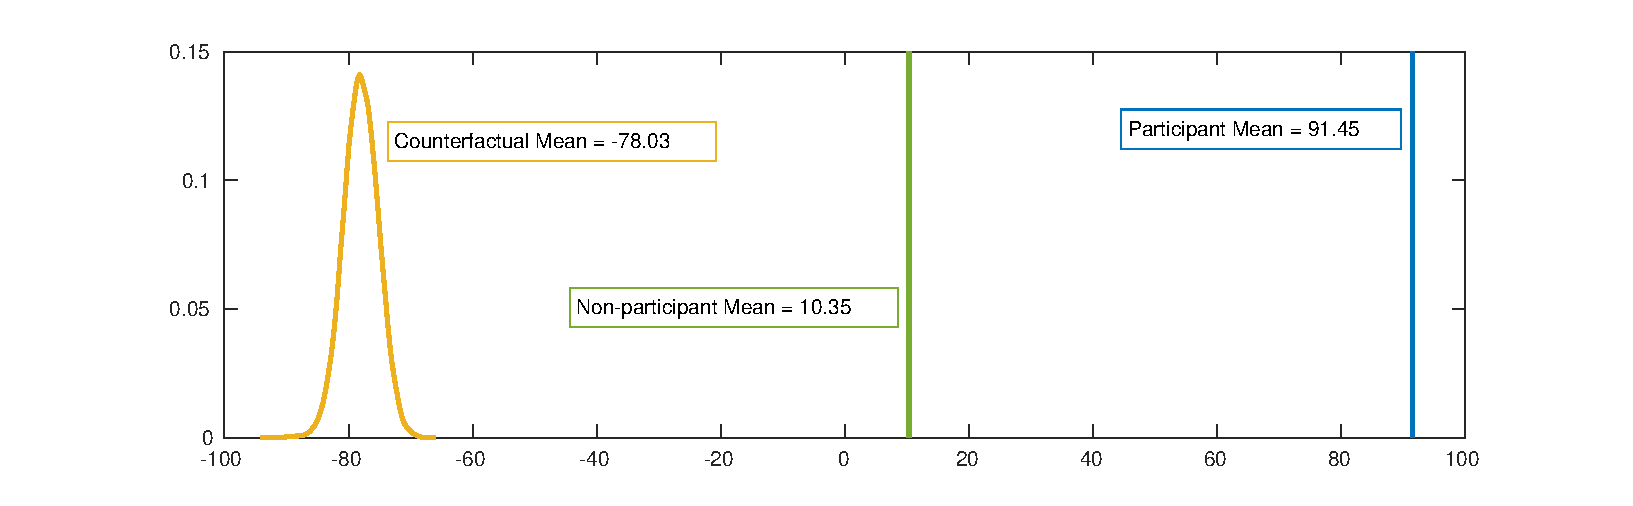
\includegraphics[scale=0.5]{./charts/counterfactual_cigwth_tech.eps}
%		\label{cigwth_c}
%	\end{center}
%	\footnotesize Chart shows the kernel density of YoY growth in C\&I loans for participating banks in the event of non-participation. The blue and green lines represent the realized average C\&I growth for participants and non-participants respectively over year ending in Q2 and Q3 2020.\\ Source: Authors' calculations.
%\end{figure}

Our counterfactual estimate of a decline of nearly 80 percent in C\&I loan books is striking. However, our estimates align with declines across loan portfolios during the Global Financial Crisis (GFC), especially among loan categories directly afflicted by the crisis. In that crisis, community banks experienced shocks to commercial real estate portfolios, and specifically to construction and land development loans \citep{Bassett2017, Friend2013}. Call report data indicate that peak-to-trough declines in C\&I and CRE loans at community banks registered at about 15 and 20 percent, respectively. Most of the run-off in CRE loans was due to declines in the most affected portfolio, construction and land development (CLD), which contracted by nearly 70 percent in total. Notably, the declines in loan balances that began during the GFC persisted for several years after the NBER recession ended.\footnote{These declines are summarized in Figure \ref{fig:CBO_gwth} with Section \ref{onappx_sec:grwth_rt_gfc} of the Online Appendix.}   

% \begin{figure}[ht]
%   \begin{center}
%    \caption{GFC Growth Rates at Community Banks}
%     \includegraphics[angle=270, scale=0.35]{./charts/CBO_growth_rates_cumulative.eps}
%     \label{fig:CBO_gwth}
%   \end{center}
% \footnotesize Note: Chart shows peak-to-trough growth rates of selected loan portfolios at community banks from the Global Financial Crisis. Peak date is 2007:Q3, the start of the NBER recession period, for all portfolios. Trough dates are the last quarter when aggregate growth was negative. Trough dates by portfolio are: C\&I, 2011:Q1; CRE, 2012:Q3; and CLD, 2013:Q1.\\ Source: Call Reports.
% \end{figure}

While our results suggest that lending would have contracted more precipitously than during the GFC, a larger and more rapid contraction in lending is consistent with the nature of the COVID shock. The onset of the pandemic induced widespread panic in financial markets \citep{Acharya2020}, causing a sudden and deep, but ultimately short-lived, recession. At its genesis, however, the pandemic looked likely to rival, and even surpass, the Global Financial Crisis in terms of economic costs.\footnote{The U.S. economy shed about 8 million jobs during the Great Recession of 2008, and over 20 million jobs during the COVID-19 recession. Source: Authors' calculations from Total Nonfarm Employees from the U.S. Bureau of Labor Statistics.} Due to the starkly weaker outlook at the onset of the pandemic, we should expect that loan growth would decline suddenly and dramatically in the ensuing period as our estimates suggest, rather than over a period of several years as seen in the Global Financial Crisis. Our findings are also in line with results from the Federal Reserve's Senior Loan Officer Opinion Survey (SLOOS) that provided evidence of a sudden tightening of lending standards.\footnote{See SLOOS results for April 2020 \url{https://www.federalreserve.gov/data/sloos/sloos-202004.htm} and July \url{https://www.federalreserve.gov/data/sloos/sloos-202007.htm}} 

\afterpage{\begin{figure}
    \caption{Estimated Counterfactual Values}
    \label{fig:ctrfct}
    \begin{subfigure}{\textwidth}
		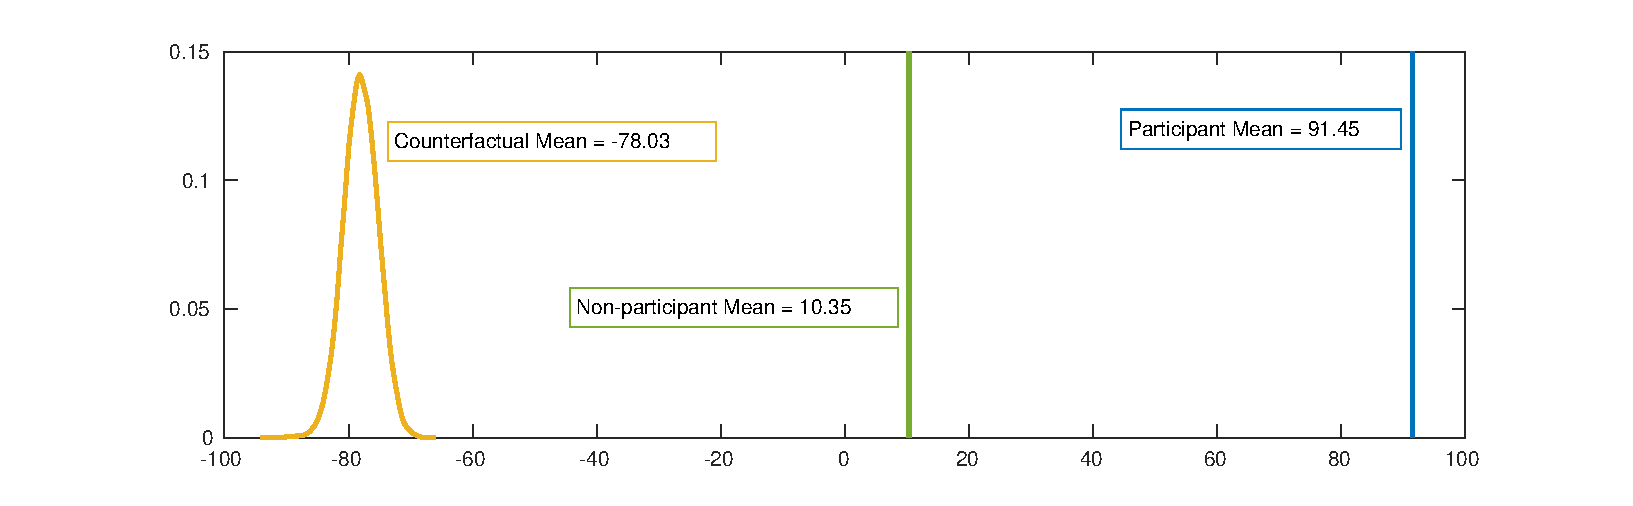
\includegraphics[scale=0.5]{./charts/counterfactual_cigwth_tech.eps}
		\caption{C\&I Loan Growth}
		\label{cigwth_c}
     \end{subfigure}
    %  \vfill
%      \begin{subfigure}{\textwidth}
%          %\begin{center}
% 		\includegraphics[scale=0.5]{./charts/counterfactual_cigwth_noppp_tech.eps}
% 		 %\end{center}
% 		 \caption{Non-PPP C\&I Loan Growth}
% 		 \label{cigwth_noppp_c}
%      \end{subfigure}
     \vfill
     \begin{subfigure}{\textwidth}
     %\begin{center}
		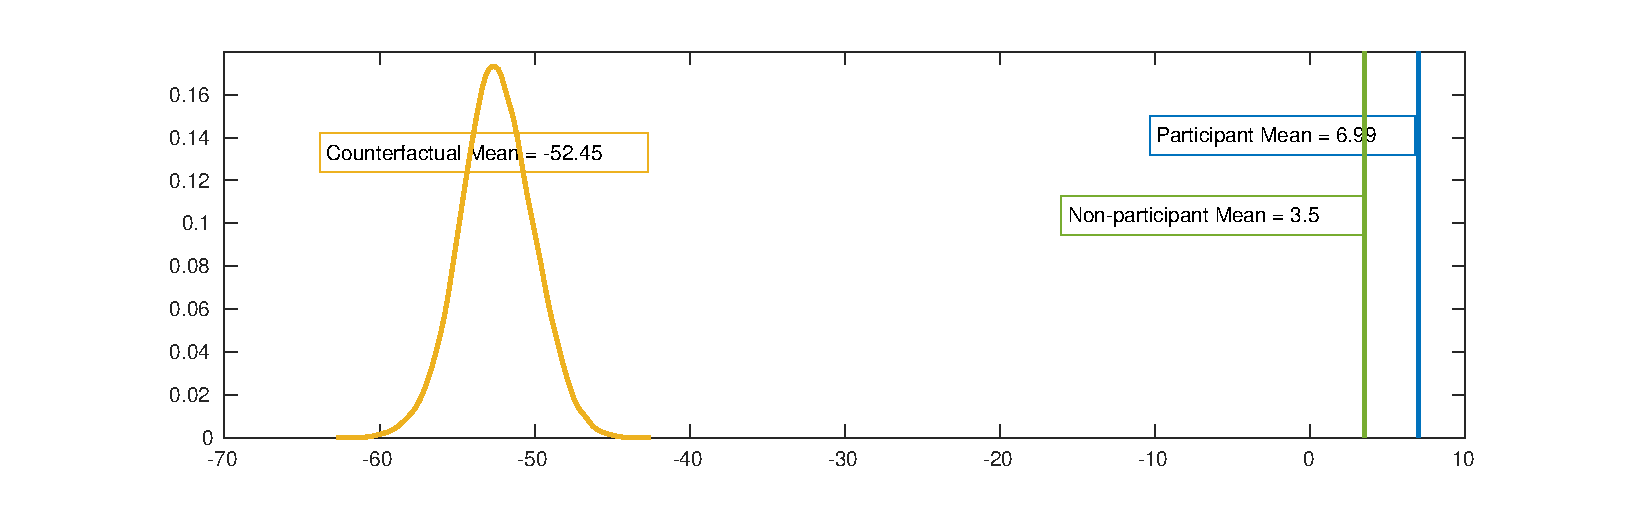
\includegraphics[scale=0.5]{./charts/counterfactual_cregwth_tech.eps}
			%\end{center}
		\caption{CRE Loan Growth}
		\label{cregwth_c}
     \end{subfigure}
     \vfill
     \begin{subfigure}{\textwidth}
      %\begin{center}
		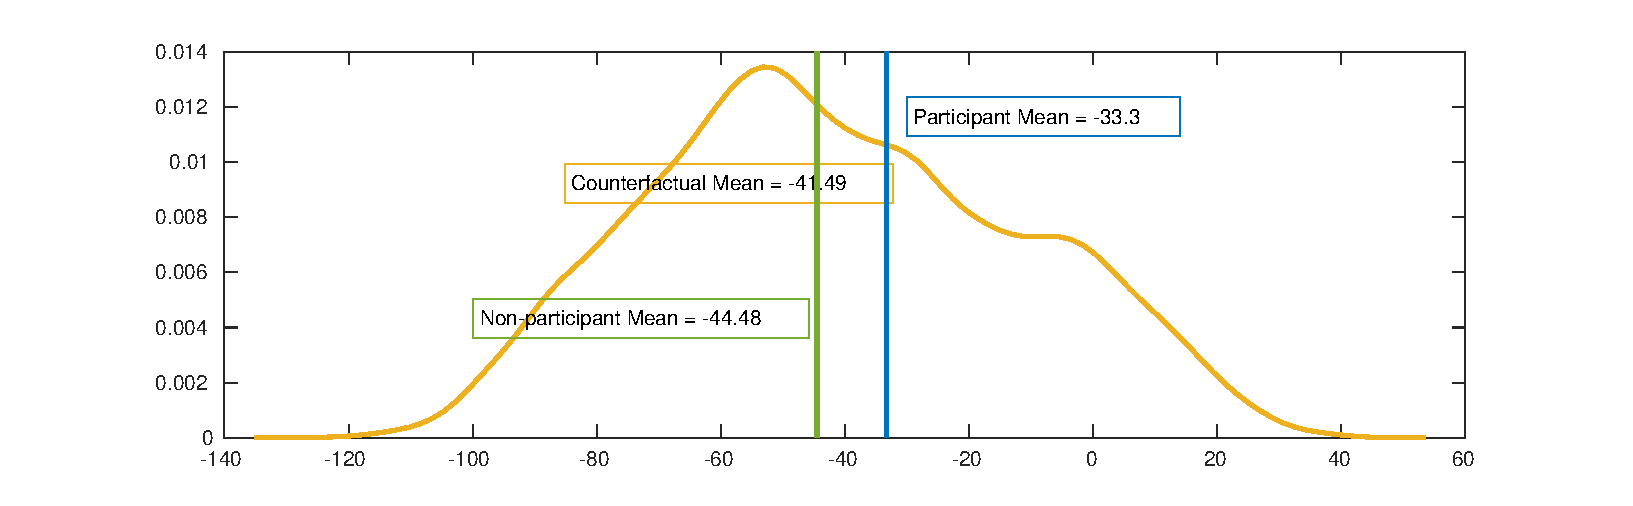
\includegraphics[scale=0.5]{./charts/counterfactual_dnim_tech.eps}
			%\end{center}
		 \caption{$\Delta$NIM}
		\label{nim_c}
     \end{subfigure}
     \\
\footnotesize Note: Charts show the posterior density of counterfactual average change in NIM for participating banks in the event of non-participation. The blue and green lines represent the realized average values for these categories for participants and non-participants, respectively, over year ending in Q2 and Q3 2020.
Source: Authors' calculations.
\end{figure}
}

%\begin{figure}[ht]
%	\begin{center}
		%\caption{Counterfactual values of Non-PPP C\&I Loan Growth}
		%\includegraphics[scale=0.5]{./charts/counterfactual_cigwth_noppp_tech.eps}
		%\label{cigwth_noppp_c}
	%\end{center}
	%\footnotesize Chart shows the posterior density of counterfactual average YoY growth in C\&I loans outside of the PPP for participating banks in the event of non-participation. The blue and green lines represent the realized average non-PPP C\&I growth for participants and non-participants respectively over year ending in Q2 and Q3 2020.\\ Source: Authors' calculations.
%\end{figure}

To look for spillovers to other business lending categories, we also examine the effects on CRE loan portfolios. We find that the PPP not only forestalled a contraction in C\&I lending, but also preempted lending declines in the CRE portfolio. Figure \ref{cregwth_c} shows that CRE lending would have declined 52 percent if participants had forgone the PPP program compared to a realized growth rate of 7 percent. This substantial difference between realized and counterfactual growth underlies our finding that the PPP had spillover effects and averted declines in lending even outside the loan category that it directly supported. 

%\begin{figure}[ht]
	%\begin{center}
	%	\caption{Counterfactual values of CRE Loan Growth}
	%	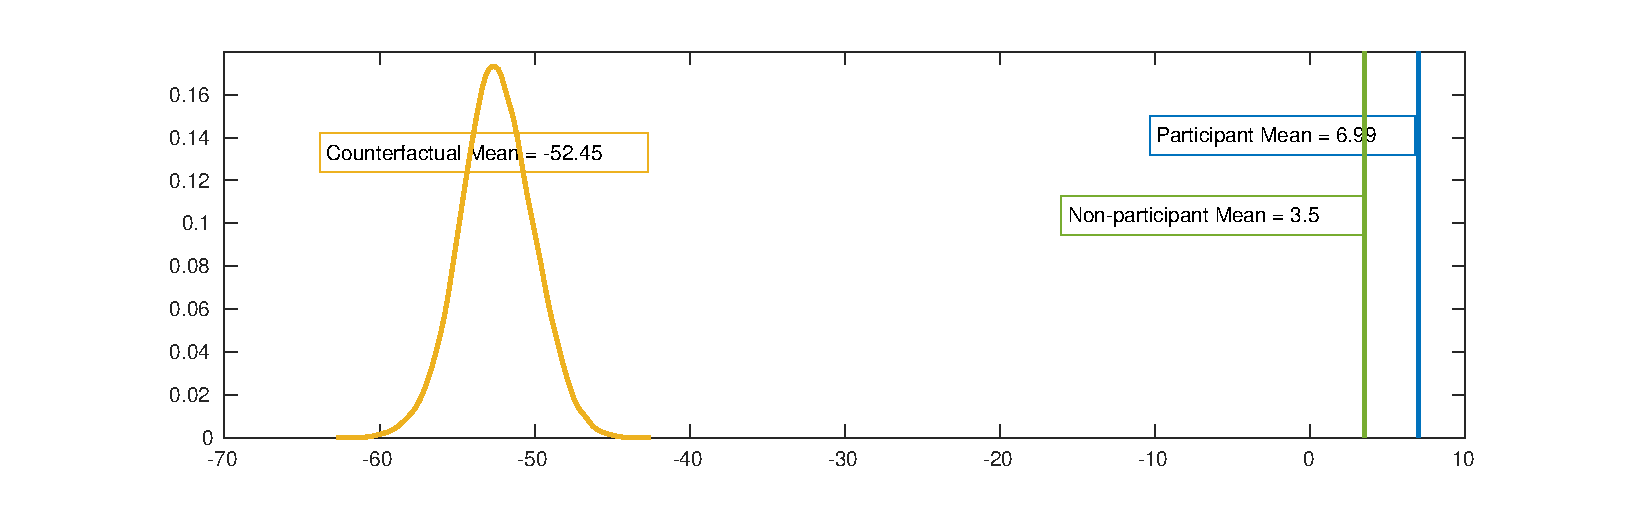
\includegraphics[scale=0.5]{./charts/counterfactual_cregwth_tech.eps}
	%	\label{cregwth_c}
	%\end{center}
	%\footnotesize Chart shows the posterior density of counterfactual average YoY growth in CRE loans outside of the PPP for participating banks in the event of non-participation. The blue and green lines represent the realized average non-PPP CRE growth for participants and non-participants respectively over year ending in Q2 and Q3 2020.\\ Source: Authors' calculations.
%\end{figure}

Consistent with the loan declines the PPP averted, we find that, on average, bank profitability was also supported by program participation. Figure \ref{nim_c} shows that participants had a realized decline in net interest margins of 33 basis points. Absent program participation however, average net interest margins were projected to decline more than 40 basis points. Although the posterior interval around this estimate spans zero, the mass of the distribution lies on the negative real line. These results demonstrate a non-linearity in the relationship between PPP lending and bank margins. In Section \ref{sec:impact}, we reported that incremental participation in the PPP compressed net interest margins. A straightforward extrapolation of this result, based only on participating banks, suggests that banks would have earned higher margins by not participating in the program. However, our counterfactual results that incorporate non-participant outcomes show that such an extrapolation would be spurious as margins would have declined further without participation. 

The decline in participants' counterfactual profit margins is partly driven by the program's revenue structure, and partly by the limited potential for profits outside the PPP during the pandemic. PPP participating banks experienced lower average C\&I loan yields, which reduced their profitability. However, the fee structure of the program helped to offset that effect. The program's unique accounting requirements entailed reporting fee income as amortized interest over the term of the loan which provided a boost to NIMs that was unavailable to non-participants. 

Outside the PPP, both diminished loan growth and depressed yields contributed to weak profit margins. Our counterfactual results suggest that participating banks' loan balances would have contracted, which would lower the denominator of NIMs. Yields on those loans would have declined sharply too, thereby compressing the entire NIM ratio. To further understand the drivers of lower NIMs outside the PPP, we decomposed NIMs of non-participant banks into share and yield effects for the C\&I, CRE, and all other loan portfolios following the methodology of \citet{covas2015net}.\footnote{In this decomposition, the share effect tells us the impact of increasing the concentration of a particular asset type, holding average yields on that asset type constant. Similarly, the yield effect tells us the change in NIM due to changes in average rates on a particular asset type, holding concentrations constant. To understand the direction of counterfactual results, we discuss the results for non-participants here. A similar decomposition for participants shows that PPP loan volumes boosted NIMs by generating revenue and fee income but average yields fell with program intensity consistent with the program's terms and unique accounting treatment of fees.} Lower loan yields, rather than change in loan shares, drove the observed decline in non-participant NIMs during our sample period. Falling loan yields are an expected consequence of low benchmark rates during the pandemic. Low interest rates typically set off a spate of refinancings or rates can automatically reset lower. In other cases, banks may have proactively lowered interest rates to remain competitive with their peers. Participating banks faced similarly falling loan yields during this time as evidenced by the decomposition results of CRE and all other loans. Our counterfactual results indicate that, had participating banks not entered the PPP, their NIMs would have suffered additional declines due to a contraction in lending volumes and consequently, in loan shares. 

In Table \ref{tab:decomp}, we examine the main drivers underlying the remarkable decline in counterfactual lending and margins for program participants.\footnote{We provide the full set of results from the decomposition in Table \ref{tab:decomp_long} in the online appendix, section \ref{onappx_sec:decomp}.} To this end, we evaluate a measure of the average contribution of each covariate to the counterfactual, namely, the product of the mean value of the covariate across participants with the estimated coefficient of that covariate for non-participants. This product is denoted by $\bar{\mathbf{x}}_{p,j}\beta_{4j}^{(g)},\hspace{2pt}g = 1,2,...,50,000$, where $\bar{\mathbf{x}}_{p,j}$ is the mean value of each covariate $j$ across participants and $\beta_{4j}^{(g)}$ is the $g^{th}$ posterior draw of the associated coefficient from equation \ref{eq:outcomes_np}. The table reports the mean and 95 percent credibility interval of this product across the 50,000 posterior draws.

\begin{table}[htbp]
  \centering
    \footnotesize
  \caption{Decomposition of predicted counterfactual outcomes for participants\label{tab:decomp}}
  \resizebox{1\textwidth}{!}{
   \begin{threeparttable}
    \begin{tabular}{rccc}
    \hline\hline
          & \multicolumn{1}{c}{$\Delta$NIM} & \multicolumn{1}{c}{C\&I Gwth}  & \multicolumn{1}{c}{CRE Gwth} \\
          \hline
& (1)   & (2)   & (3) \\
\hline\hline
     \multicolumn{1}{l}{ln Assets} & -11.39 & -93.5 & -46.49 \\
          & [-62.41, 44.45] & [-105.88, -81.22] & [-55.21, -37.8] \\
    \multicolumn{1}{l}{ALLL to Total Loans} & -12.72 & -2.72 & -1.24 \\
          & [-16.15, -9.25] & [-6.09, 0.59] & [-3.38, 0.91] \\
          \hline\hline
    \end{tabular}%
       \begin{tablenotes}
        \footnotesize \item Note: The reported values are posterior means of the product of covariates and parameters, and 95\% credibility intervals in brackets. The results are based on 55,000 MCMC draws with a burn-in of 5000.  
    \end{tablenotes}
\end{threeparttable}
    }
\end{table}%


Our decomposition of the counterfactual outcomes reveals two important findings. First, bank size and loan loss allowances predominantly explain the full magnitude of counterfactual lending and margins. Second, the relationship between bank characteristics and outcomes is  fundamentally different across participants and non-participants. Together with the differences in the pre-pandemic characteristics across the two groups of institutions, these differences in relationships explain why participating banks would have contracted their loan portfolios and faced greater margin compression if they had not engaged in the PPP compared to banks that actually opted out of the program.

Bank size largely explains the sharply lower counterfactual margins and loan growth for participants relative to their realized outcomes. Contrary to participants, margins and loan growth declined with size among non-participants. Moreover, participating banks are larger than non-participants. Taken together, the model predicts that the mean participants' asset size would have contributed to a decline in NIM of 11 basis points relative to 2019, and a reduction in C\&I and CRE loan portfolios by 94 percent and 46 percent, respectively, had they not participated in the PPP. This result points to differences in the way small and large community banks responded to the crisis. Smaller banks, which were less likely to participate in the program, continued to lend using their own capital. Larger banks were more likely to participate in the PPP, however, and those that did not engage in the program curtailed lending. Therefore, participating banks, which were relatively larger in size, would have retrenched lending and undergone further compression in margins if they had not engaged in the PPP.   

The second salient factor underlying participants' counterfactuals is the ratio of loan loss allowances to total loans. Participating banks with average ALLL ratios were likely to undergo a 13 basis point decline in NIM relative to 2019, and declines of 3 and 1 percentage points in C\&I and CRE loan growth respectively. Loan loss allowances were, on average, higher among non-participants and were negatively associated with loan growth and profit margins among both participants and non-participants. Notably, incremental loan loss allowances as a share of loans were associated with a larger decline in margins among non-participants relative to participants. Taken together, participants' loan loss allowances would have resulted in a larger decline in NIMs in the counterfactual case of non-participation relative to actual declines under participation. Loan loss allowances likely restricted non-participants' ability to engage in risk-taking, diminishing their margins. Participants, on the other hand, were likely able to issue riskier, higher-yielding loans owing to the risk-free nature of PPP loans which moderated the negative effect of loan loss allowances on bank margins. 

Contrary to NIM, the magnitude of the loan growth decline in response to loan loss allowances was lower under non-participation compared to the decline predicted under participation. Because loan growth was substantially lower under non-participation, bank funding requirements would have been lower under this scenario, and loss allowances would have constrained lending by a lesser extent. Our results show that if participants had foregone the PPP, banks already exposed to potential losses would have continued to withhold lending, albeit to a lesser extent than if they had participated in the program.\footnote{We discuss the distinct effects of parameters and covariate values on counterfactual estimates in the online appendix, section \ref{appx_subsec:counterfact_discuss}.}

The counterfactual values for bank lending are consistent with our finding that bank participation in the PPP was motivated by risk-aversion, suggesting that the program likely did not crowd out private lending. To be sure, if banks had not participated in the PPP, even as they allowed loans to run off, they would have continued some lending as evidenced by the substantial liquidity they provided through credit line drawdowns early in the pandemic. But even these drawdowns were concentrated among larger firms that were less exposed to pandemic-induced losses rather than smaller firms that were the targets of PPP loans \citep{LiStrahanZhang2020, chodorow2021bank}. This suggests that rather than crowd out private lending, the PPP addressed unmet credit needs of small firms. Alternatively, the program may have suppressed bank loan balances if borrowers used the funds to repay existing loans even though such usage would disqualify them from loan forgiveness. In the absence of detailed loan-level data from community banks, we cannot explicitly measure this effect. We note, however, that the PPP incorporated features that would have induced, rather than crowded out, private lending by participants. The program supported the balance sheets of recipients and their eligibility for credit from risk-averse banks. Because PPP loans were free of credit risk, banks were able to maintain other non-guaranteed lending, as suggested by our treatment effects. This means the PPP, crucially, did not crowd out all private lending. 

Instead, the PPP offset what would have been a sharp decline in bank lending, a result that is consistent with evaluations of other COVID-era support programs. For example, \cite{Minoiu2021} find that, despite low take up, the Main Street Lending Program (MSLP) functioned as a backstop by stimulating lending outside of the program. We find that the PPP helped more directly offset a credit contraction by encouraging lenders to utilize the program. Further, our counterfactual results highlight the limitations of relationship lending during crises. Our counterfactual results confirm that, in fact, absent the PPP, bank lending to businesses would have contracted substantially. While existing relationships measured by C\&I lending exposures would have mitigated this effect to some degree, they could not fully offset the credit crunch that would have occurred absent the PPP.





\section{Robustness\label{sec:robust}}

%We further verify our results on bank outcomes . 

In this section, we reexamine our identifying assumptions and empirical approach by conducting a battery of robustness checks on bank outcomes. To do so, we consider alternatives to the two instruments in our model. We also assess the program's different phases by examining outcomes across each program quarter separately. Next, we reassess loan demand controls by adding drawdown measures. Finally, we conduct a subsample analysis along lending and capital dimensions to highlight the importance of these characteristics in determining participant banks' outcomes.  

\subsection{Alternative Instruments\label{subsec:alt_instruments}}

In the PPP participation equation, we consider two alternative instruments based on SBA lending in line with recent PPP research. The first is the share of SBA volume to total small business C\&I loan volume over the five years prior to the pandemic. This is similar to the instrument used in \cite{Lopez2021}, except that the authors base their instrument on this ratio for 2019. The second instrument is analogous to the first, where we evaluate the ratio of the number, instead of the volume, of SBA loans to small business C\&I loans.  \cite{Granja2020} used a similar instrument in their study over a three year, pre-pandemic period. Overall, SBA-lending based instruments are appealing because they reflect an important institutional feature of the PPP: banks were automatically eligible to participate in the PPP if they were previously certified as SBA 7(a) lenders \citep{Lopez2021, barraza2020short}.  

Table \ref{tab:instComp1} shows that both the share of SBA loan volumes and counts are positively associated with PPP participation. In addition, the treatment effect estimates for C\&I lending are close to the range reported using our baseline instrument. While our results are robust to alternative instruments used in the literature, we highlight a caveat with the use of the SBA-based instruments revealed by our investigation of the loan-level data from the 7(a) program. The number of active SBA relationship lenders has been declining over the last decade, with fewer than 1,500 active lenders each year since 2014. Over a five-year horizon, only 45 percent of participating banks in our sample have a non-zero entry for SBA lending ratios, and the share of active lenders in 2019 alone is even lower, at 24 percent. These shares are substantially lower than the fraction of participating banks reporting technological expenses, at 89 percent, which underlies our main instrument. Therefore, familiarity with SBA systems over the pre-pandemic horizon likely explains an important, but limited, share of the ultimate PPP participation rate.   

 % Table generated by Excel2LaTeX from sheet 'compare_instruments'
\begin{table}[htbp]
	\centering
	\caption{Alternatives to the  Instrument for PPP Participation\label{tab:instComp1}}
	\resizebox{0.9\textwidth}{!}{
		\begin{threeparttable}
	\begin{tabular}{lccc}
	    \hline\hline
		& Tech. exp. to assets & \multicolumn{1}{l}{SBA loan vol share (5 yr)} & \multicolumn{1}{l}{SBA loan count share (5 yr)} \\
		\hline
          & (1) & (2) & (3) \\
          \hline\hline
	\multicolumn{1}{l}{Effect on PPP participation} & -0.165 & 0.001 & 0.005 \\
& [-0.26, -0.07] & [0, 0.003] & [0, 0.01] \\
\multicolumn{1}{l}{Treatment effect} & 10.523 & 10.493 & 10.689 \\
& [9.26, 11.87] & [9.01, 11.84] & [8.85, 12.48] \\
    \hline\hline
	\end{tabular}%
	\begin{tablenotes}
		\item Note: Effect on PPP participation is obtained from equation \ref{eq:select}, and the treatment effect, from  \ref{eq:outcomes_p} of the Bayesian joint model. 95\% credibility intervals are shown in brackets. 
	\end{tablenotes}
\end{threeparttable}
}
\end{table}%

 
 We extend our robustness exercise into the second step of our model by considering three alternatives to our instrument for PPP intensity. First, we calculate the share of small firm employment in a bank's operating region to measure PPP demand, analogous to our main instrument for intensity based on COVID-affected employment share. Indeed, this alternative variable is constructed in the same fashion as our main instrument, by weighting county-level small firm employment by a bank's deposit share in each county. To evaluate this measure, we use data from QWI to identify firms with fewer than 500 employees, which roughly corresponds to the employment-based threshold used to determine small firm PPP eligibility. Second, we use a bank's core deposit-to-assets ratio, which measures a bank's ability to fund PPP loans without additional capital market activity. Finally, we consider the share of unused commitments to total assets. This variable captures a bank's exposure to potential pandemic-induced drawdowns. Banks are more likely extend PPP loans to customers with higher drawdowns because PPP loans shift risks from bank balance sheets to the government's without severing customer relationships. We recognize, a priori, that the two bank-level instruments are not exogenous to the bank's decision on participation intensity, but use the direction of the ensuing results to benchmark our main estimates. 

Table \ref{tab:instComp} shows the effect of our main instrument as well as the three alternatives on participation intensity and C\&I loan growth. Small firm employment is negatively related to PPP intensity suggesting that the presence of small firms in a bank's operating region does not adequately represent program demand. Indeed, employment-based eligibility thresholds may have been designed to target firms with deficient access to finance, giving rise to the negative estimated relationship. Banks located in regions with predominantly credit-constrained firms would have been more likely to ration credit rather than expand lending. Bank balance sheet measures reflect the selection effects we had previously highlighted. Banks with greater core deposit shares, and thereby more resources to lend, and those with higher shares of unused commitments, representing higher potential loan loss exposures, were more intensive PPP lenders. Funding capacity and loss exposure also represent important bank characteristics that directly affect C\&I loan growth, thereby breaching the exclusion restriction. This endogeneity likely contributed to the lower magnitude of treatment effects under the bank measures. Overall, alternative instruments yield positive, statistically important treatment effects, but underscore the validity of our main instrument.\footnote{In the online appendix, section \ref{appx_subsec:ext_robust}, we report results based on a specification that includes all instruments for intensity and participation under the Bayesian setting, and an equivalent IV setting with all instruments for intensity. We find that the instruments retain their statistical importance. Treatment effects, while moderately attenuated, are largely unchanged from baseline.}     

 % Table generated by Excel2LaTeX from sheet 'instrument relevance'
\begin{table}[htbp]
  \centering
  \caption{Alternatives to the  Instrument for PPP Intensity\label{tab:instComp}}
  \resizebox{0.9\textwidth}{!}{
  \begin{threeparttable}
    \begin{tabular}{lcccc}
    \hline\hline
          %& \multicolumn{1}{p{5.4em}}{Small firm employment share} & \multicolumn{1}{p{5.4em}}{COVID-affected employment share} & \multicolumn{1}{p{5.7em}}{Core Deposits to Assets} & \multicolumn{1}{p{5.6em}}{Unused CI Commitments to Assets} \\
          & COVID-affected & Small firm & Core Deposit & Unused C\&I Cmmt \\
          &Employment & Employment & Ratio & Ratio \\ \hline
          & (1) & (2) & (3) & (4) \\
          \hline\hline
    Effect on PPP intensity  &  0.082 & -0.074 & 0.069 & 0.526 \\
     & [0.06, 0.1] & [-0.09, -0.06] & [0.06, 0.08] & [0.47, 0.58] \\
         Treatment effect & 10.523 & 12.316 & 6.243 & 6.307 \\
      & [9.26, 11.87] & [10.72, 13.84] & [4.65, 7.78] & [5.21, 7.37] \\
    \hline\hline
    \end{tabular}%
    \begin{tablenotes}
     \item Note: Effect on PPP intensity is obtained from equation \ref{eq:ppp_int}, and the treatment effect, from  \ref{eq:outcomes_p} of the Bayesian joint model. 95\% credibility intervals are shown in brackets.
    \end{tablenotes}
    \end{threeparttable}
    }
\end{table}%




 \subsection{Program Timing Effects\label{subsec:program_timing}}

We investigate the timing of the PPP's effects on bank outcomes in Table \ref{tab:robustness_qtr_outcomes}. While early access to the program was critical for firms to withstand the disruptions from the pandemic\citep{balyuk2021small, Doniger2021}, we find that the timing of PPP lending was also relevant to banks' profitability. We split our sample period into subsamples for 2020:Q2 and 2020:Q3, the quarters when the program was most active.\footnote{Additional details about the individual quarter estimates are available in the online appendix, section \ref{onappx_sec:qtr_bayes}. Results for the fourth quarter of 2020, which is not considered in our main sample, are presented in the online appendix \ref{appx:q4_bayes}.} The first column shows that the decline in NIM we had previously reported occurred almost entirely in the second quarter of 2020. Lending growth, however, did not vary across the two quarters. C\&I lending consistently grew year-over-year in both quarters as shown by column (2). Similarly, columns (3) and (4) show that the program had only a modest effect on lending outside of the program in both quarters. Our results suggest that banks' margins declined when they swiftly disbursed a large number of loans early in the pandemic, when economic activity was restricted, and financial markets were in turmoil. But, as economic activity increased and demand for loans stabilized, banks likely improved their processes to assess  applications based on their profit margin impact. In addition, loan sizes declined in later PPP rounds which increased the relative fee size and helped to further support bank margins.   

% Table generated by Excel2LaTeX from sheet 'Sheet1'
\begin{table}[htbp]
  \centering
  \caption{Quarterly Treatment Effects by Outcome\label{tab:robustness_qtr_outcomes}}%
  \resizebox{0.9\textwidth}{!}{
  \begin{threeparttable}
    \begin{tabular}{rcccc}
    \hline\hline
     & $\Delta$NIM(bps)  & C\&I Gwth(\%) & Non-PPP C\&I Gwth(\%) & CRE Gwth(\%) \\ \hline
            & (1) & (2) & (3) & (4) \\ \hline
    \hline
    $\text{\emph{Baseline}}$ & \multicolumn{1}{c}{-4.27} & \multicolumn{1}{c}{10.52} & \multicolumn{1}{c}{-0.46} & \multicolumn{1}{c}{0.23} \\
          & [-6.03, -2.7] & [9.26, 11.87] & [-1.46, 0.57] & [-0.54, 1.01] \\
		$\text{\emph{Q2 2020}}$ & -6.91 & 10.72 & 0.36  & 0.20 \\
		& [-9.15, -4.92] & [8.65, 12.92] & [-0.89, 1.71] & [-0.71, 1.09] \\
		$\text{\emph{Q3 2020}}$ & -0.19 & 9.53  & -0.33 & 0.41 \\
		& [-2.54, 2.39] & [7.18, 12.04] & [-2.33, 1.54] & [-0.76, 1.61] \\
          \hline\hline
    \end{tabular}%
    \begin{tablenotes}
        \footnotesize \item Note: The reported values are posterior means of the parameters, and 95\% credibility intervals in brackets. The results are based on 55,000 MCMC draws with a burn-in of 5000. 
    \end{tablenotes}
\end{threeparttable}
    }
\end{table}%


\subsection{Credit Line Drawdown Effects\label{subsec:drawdowns}}

We reevaluate our treatment effects by controlling for the sharp rise in credit line drawdowns that banks experienced in the first quarter of 2020. Table \ref{tab:robustness_ci_draws} reports our baseline result for PPP intensity as well as estimates from a model that includes an indicator for banks in the top quartile of C\&I growth in 2020:Q1. We find that after controlling for large drawdowns, the negative effect of the PPP on profit margins is only slightly attenuated. This suggests that declining profitability during the PPP's operational period was not due to a sudden expansion of the asset base from drawdowns. In fact, total C\&I loan growth was higher in the specification that controls for large C\&I drawdowns. However, columns (3) and (4) show that the effect of the PPP on lending outside of the program remained muted even after controlling for credit line drawdowns. Therefore, the effects of the PPP on lending growth remain broadly unchanged after addressing the conversion of off-balance sheet commitments into on-balance sheet exposures due to firm credit line usage.\footnote{The online appendix, section \ref{onappx_sec:2020Q1_Loan_Draws} summarizes the direct effect of drawdowns on participation, intensity, and bank outcomes controlling for other characteristics. We find that banks that experienced large drawdowns were more likely to participate in the PPP, as well as undergo larger growth in C\&I loans and larger change in NIM relative to 2019.}

\subsection{Subgroup Analysis\label{subsec:subgroups}}

We evaluate the PPP's effects across bank characteristics by performing a subsample analysis based on bank size, capital constraints and specialty. The results from this analysis are reported in the online appendix, section \ref{onappx_sec:subsample}. Lending growth was larger at smaller banks, institutions less constrained by the leverage ratio, and those with a specialty in CRE lending. Base effects likely underlie the relatively lower growth rate in lending among larger banks and those with larger C\&I loan concentrations. Because these bank groups had larger pre-pandemic C\&I loan volumes, every PPP loan dollar generated a lower growth rate relative to banks with small C\&I loan stocks.

% Table generated by Excel2LaTeX from sheet 'Sheet1'
\begin{table}[htbp]
  \centering
  \caption{C\&I Loan Draw Effects\label{tab:robustness_ci_draws}}%
  \resizebox{0.9\textwidth}{!}{
  \begin{threeparttable}
    \begin{tabular}{rcccc}
    \hline\hline
     & $\Delta$NIM(bps)  & C\&I Gwth(\%) & Non-PPP C\&I Gwth(\%) & CRE Gwth(\%) \\\hline
        & (1) & (2) & (3) &4) \\ \hline\hline
    \multicolumn{1}{l}{Baseline} & \multicolumn{1}{c}{-4.27} & \multicolumn{1}{c}{10.52} & \multicolumn{1}{c}{-0.46} & \multicolumn{1}{c}{0.23} \\
          & [-6.03, -2.7] & [9.26, 11.87] & [-1.46, 0.57] & [-0.54, 1.01] \\
    \multicolumn{1}{l}{Baseline + CI gwth top qrtile} & \multicolumn{1}{c}{-3.92} & \multicolumn{1}{c}{12.13} & \multicolumn{1}{c}{0.20} & \multicolumn{1}{c}{0.29} \\
          & [-5.45, -2.37] & [10.67, 13.61] & [-0.78, 1.17] & [-0.46, 0.99] \\
          \hline\hline
    \end{tabular}%
    \begin{tablenotes}
      \item Note: The reported values are posterior means of the parameters, and 95\% credibility intervals in brackets. The results are based on 55,000 MCMC draws with a burn-in of 5000.  
    \end{tablenotes}
    \end{threeparttable}
    }
\end{table}%





 

\section{Discussion and Policy Implications\label{sec:conclude}}
Under the Paycheck Protection Program, banks issued business loans that could later be fully forgiven and reimbursed with federal funding. Banks—- especially small community banks—- participated extensively, with PPP loans representing nearly all new lending in 2020. However, the program’s effects on community banks' balance sheets have not been fully understood. 

Our results show that the PPP not only supported businesses, but also the banks that disbursed the loans. Although the PPP carried a low interest rate, the program ensured a modest revenue stream for participating banks when safe and profitable lending opportunities were scarce. At the same time, by guaranteeing credit extensions, the program avoided a credit crunch at small and mid-sized businesses when revenues were falling quickly. Overall, the PPP indirectly provided crucial support to community banks in the form of income and credit growth and likely protected banks from business-related credit losses during the height of the pandemic. 
In addition, we find that community banks with ample funding—namely, larger and more profitable banks—were more likely to participate in the PPP; however, participating community banks with weak capital originated more PPP loans relative to their size. This suggests the PPP helped mitigate risk for weaker banks at a time of high economic and financial uncertainty. 

The PPP experience highlights important lessons for the structure of future government lending programs. First, loan guarantee programs generate important consequences for the distribution of funds, particularly when those programs are implemented as emergency lending measures in response to a crisis. Policymakers may be forced to prioritize timeliness over targeting efficiency, resulting in funds flowing to geographical areas and firms whose need may not be the highest \citep{Granja2020, Joaquim2022}. Indeed, banks may have been incentivized to transfer substantial risks to the federal government and lend to firms of weak credit quality as was found to be the case in Japan \citep{honda2023determinants, hoshi2021return}. Our datasets do not permit an evaluation of the quality of firms that ultimately received the loans. However, we do find selection effects among banks that elected to participate in the PPP. Because larger and more profitable community banks were more likely to participate in the program, the initial program wave likely did not reach the smallest borrowers that are usually serviced by the smallest community banks. In addition, banks that were relatively weakly capitalized were also more likely to participate in the program. Accordingly, the broad-based eligibility of the program was especially suited for an exogenous crisis like the COVID-19 shock. If such a program were offered following a financial shock such as the Global Financial Crisis, weakly managed, at-risk banks may have used the program to gamble for resurrection. 

Second, guarantee program parameters must balance participation incentives with those for underwriting. One likely reason for widespread PPP take-up was the program's broader implicit guarantee relative to standard guarantee programs. European guarantee programs that operated contemporaneously with the PPP, and prior programs in Japan, did not convert loans to grants by means of a forgiveness procedure \citep{ono2013lending, core2021public}. Indeed, other programs provided only partial guarantees for loans above a threshold. Despite the more generous nature of the PPP's loan guarantees, which likely encouraged greater bank and firm participation, other features of the program placed costs on participating banks and held excessive risk transfer to the federal government in check. Our findings show that bank profitability declined with PPP participation intensity. Low interest rates and fee deferrals until forgiveness diluted margins, but also likely curtailed incentives for originating poor-quality loans that may have later been deemed ineligible for forgiveness. Similarly, requiring banks to initially use their own capital to originate these loans also likely served to reduce moral hazard incentives. 
 
Third, government guarantees serve as an antidote to a credit crunch in times of severe economic uncertainty. Our counterfactual analyses show that, absent the PPP, small businesses would have likely faced steep credit access constraints during the pandemic. 
 
Overall, the PPP serves as a new tool that may be used in times of a large, exogenous shock to the economy. Future uses of this program may require adjusting loan terms to ensure credit support while disincentivizing moral hazard. 


% References
\end{onehalfspace}
\clearpage
\bibliographystyle{abbrvnat}
\bibliography{bibliography}

%% Appendix 
\begin{onehalfspace}
\clearpage
\pagebreak
\appendix
\renewcommand{\thesection}{\Alph{section}}
\clearpage

\section{Bayesian Joint Model Estimation Details\label{appx:Bayesian_MCMC}}
\setcounter{table}{0}
\setcounter{figure}{0}
\setcounter{equation}{0}
\renewcommand{\thetable}{A.\arabic{table}}
\renewcommand{\thefigure}{A.\arabic{figure}}
\renewcommand{\theequation}{A.\arabic{equation}}

This appendix presents the Bayesian joint model details.

\subsection{Bayesian Joint Model Setup Details}

The model measures the effect of the PPP on bank loan growth and profits by controlling for changes in those measures that arise from bank decisions rather than the program's features. Banks decided whether and how much to participate in the PPP due to the voluntary nature of the program. These decisions introduce a selection bias, and render the main treatment variable endogenous. We address these econometric challenges by modeling banks' decisions to participate in the PPP, and their choice of PPP intensity, jointly with the effect of PPP on bank outcomes.  Figure \ref{dag} illustrates the structure of our statistical model. Equation (1) defines the decision to participate in the PPP, equation (2) models the intensity of participation, equation (3) models the financial outcomes of participants, and equation (4) models the outcomes of non-participants. 

\begin{figure}[ht]
  \begin{center}
   \caption{Joint model of PPP participation, intensity, and bank outcomes}
    \includegraphics[, scale=0.6]{./charts/dag.jpg}
    \label{dag}
  \end{center}
\end{figure}

By modeling participation and intensity in two separate equations, we allow for the possibility that bank characteristics may distinctively affect the two decisions. Our model follows the multivariate structure in \cite{vossmeyer2016sample} for sample selection and treatment, but specifies a continuous treatment instead of a censored treatment. The model structure in Figure \ref{dag} is formally represented by Equations \ref{eq:select} - \ref{eq:outcomes_np}. The control variables $\mathbf{x'_{i}}$ are common to all four equations and consist of pre-determined bank and operating region characteristics. We specify a multivariate normal distribution, $\mathcal{N}_{4}(0,\mathbf{\Omega})$, for the errors $\epsilon_{i} =(\epsilon_{i1},\epsilon_{i2},\epsilon_{i3},\epsilon_{i4})$.  

One of the main advantages of undertaking a joint modeling approach is that it allows us to incorporate covariances between outcomes across Equations \ref{eq:select} - \ref{eq:outcomes_np}. The covariance matrix $\mathbf{\Omega}$ depicts the relationships between unobservables $\epsilon_{i} =(\epsilon_{i1},\epsilon_{i2},\epsilon_{i3},\epsilon_{i4})$. 
\begin{equation}
	\mathbf{\Omega} = \begin{pmatrix}
	1 & \Omega_{12} & \Omega_{13} & \Omega_{14}\\
	\Omega_{21} & \Omega_{22} & \Omega_{23} & \centerdot\\
	\Omega_{31} & \Omega_{32} & \Omega_{33} & \centerdot\\
	\Omega_{41} & \centerdot & \centerdot & \Omega_{44}\\
	\end{pmatrix}\label{eqn:covar}
\end{equation} 

 The term $\Omega_{12}$ measures the covariance between unobservables underlying the decision to participate and the intensity of participation. The covariance terms $\Omega_{13}$ and $\Omega_{14}$ record the relationship between unobservables pertaining to the decision to participate and bank outcomes for participants and non-participants, respectively. The covariance term $\Omega_{23}$ records the effect of unobservables across the intensity of participation in the PPP and bank-level outcomes. The elements $\Omega_{24}$ and $\Omega_{34}$ are not identified as they correspond to covariances across outcomes for participants and non-participants, which are mutually exclusive.

We obtain the likelihood for this model by partitioning the equations into outcomes and covariates pertaining to participants and non-participants. We denote $N_{p}$ and $N_{np}$ as the set of participant and non-participant banks in the sample. The complete-data likelihood function for the full sample of observations combines the elements pertaining to each group of banks,
 \begin{equation}
     f(y, y_{1}^{*} \vert \mathbf{x_{i}}, \theta, \Omega_{p}, \Omega_{np}) = \prod_{i \in N_{p}}\left[f_{\mathcal{N}}(\bm{y}_{i,p} \vert \mu_{i,p}, \Omega_{p})\right]\prod_{i \in N_{np}}\left[f_{\mathcal{N}}(\bm{y}_{i,np} \vert \mu_{i,np}, \Omega_{np})\right].
 \end{equation}

We assign independent multivariate normal priors to the coefficients $f(\theta) = f_{\mathcal{N}}(\theta\vert\Theta_{0},T_{0})$, where $\theta = [\gamma_{1}, \gamma_{2}, \delta, \boldsymbol{\beta}]$, and $\boldsymbol{\beta} = \{\beta_{1},\beta_{2},\beta_{3},\beta_{4}\}$. The covariance matrices $\Omega_{p}$ and $\Omega_{np}$ are assigned Inverse Wishart priors, $f(\Omega_{p}) = f_{\mathcal{IW}}(\Omega_{p}\vert \nu_{p}, Q_{p})$, and $f(\Omega_{np}) = f_{\mathcal{IW}}(\Omega_{np}\vert \nu_{np}, Q_{np})$, which are independent of priors assigned to the coefficients. On combining the complete-data likelihood, and priors, we obtain the augmented posterior as follows.

 \begin{equation}
     f(\theta, \Omega_{p}, \Omega_{np}, y_{1}^{*} \vert y) \propto f(y, y_{1}^{*} \vert \mathbf{x_{i}}, \theta, \Omega_{p}, \Omega_{np})f(\theta)f(\Omega_{p})f(\Omega_{np})
 \end{equation}

\subsection{Estimation Algorithm}

To implement the estimation algorithm, we partition the full set of outcomes into those that pertain to participants and non-participants, $\bm{y}_{i,p}$, and $\bm{y}_{i,np}$, respectively, where,
\begin{equation}
    \bm{y}_{i,p} = \begin{pmatrix}
    y_{i1}^{*}\\y_{i2}\\y_{i3}\\
    \end{pmatrix}, \hspace{10pt} \bm{y}_{i,np} = \begin{pmatrix}
    y_{i1}^{*}\\y_{i4}\\
    \end{pmatrix}\label{eq:outcomes_grp}.
\end{equation}
The marginal mean of each set of outcomes based on equations \ref{eq:select} - \ref{eq:outcomes_np} is obtained from the following expressions.
\begin{equation}
    \mu_{i,p} = \begin{pmatrix}
    \mathbf{x'_{i}\beta_{1}}+ z_{i1}\gamma_{1}\\ \mathbf{x'_{i}\beta_{2}}+ z_{i2}\gamma_{2}\\\mathbf{x'_{i}\beta_{3}}+ y_{i2}\delta\\
    \end{pmatrix}, \hspace{10pt} \mu_{i,np} = \begin{pmatrix}
    \mathbf{x'_{i}\beta_{1}}+ z_{i1}\gamma_{1}\\\mathbf{x'_{i}\beta_{4}}\\
    \end{pmatrix}\label{eq:covar_grp}.
\end{equation}
We consider the elements of the covariance matrix pertaining to participants and non-participants separately and label them $\Omega_{p}$ and $\Omega_{np}$, respectively. Accordingly, the two covariance matrices are defined as,
\begin{equation}
	\Omega_{p} = \begin{pmatrix}
		1 & \Omega_{12} & \Omega_{13}\\
		\Omega_{21} & \Omega_{22} & \Omega_{23}\\
		\Omega_{31} & \Omega_{32} & \Omega_{33}\\
	\end{pmatrix}, \hspace{10pt} 	\Omega_{np} = \begin{pmatrix}
	1 & \Omega_{14}\\
	\Omega_{41} & \Omega_{44}\\
\end{pmatrix}\label{eq:var_grp}.
\end{equation} 

Subsequently, we rearrange the data in a Seemingly Unrelated Regressions setup \citep{zellner1962efficient}. The rearranged covariate matrices are,
\begin{equation}
    \mathbf{X}_{i,p} = \begin{pmatrix} \mathbf{x'_{i}} & z_{i1} & \mathbf{0} & 0 & \mathbf{0} & \mathbf{0}\\ \mathbf{0} & 0 & \mathbf{x'_{i}} & z_{i2} &  \mathbf{0} & \mathbf{0}\\ \mathbf{0} & 0 & \mathbf{0} &  0 & \mathbf{x'_{i}} & \mathbf{0}\\
    \mathbf{0} & 0 & \mathbf{0} &  0 & \mathbf{0} & \mathbf{0}\end{pmatrix}, \hspace{5pt} \mathbf{X}_{i,np} = \begin{pmatrix} \mathbf{x'_{i}} & z_{i1} & \mathbf{0} & 0 & \mathbf{0} & \mathbf{0}\\ \mathbf{0} & 0 & \mathbf{0} & 0 &  \mathbf{0} & \mathbf{0}\\ \mathbf{0} & 0 & \mathbf{0} & 0 &  \mathbf{0} & \mathbf{0}\\ \mathbf{0} & 0 & \mathbf{0} &  0 & \mathbf{0}  & \mathbf{x'_{i}} \end{pmatrix}.
\end{equation}

The outcomes are stacked into vectors $\bm{Y}_{i,p}$ and $\bm{Y}_{i,np}$,
\begin{equation}
    \bm{Y}_{i,p} = \begin{pmatrix} y_{i1}^{*}\\y_{i2}\\y_{i3}\\0\end{pmatrix}, \hspace{5pt} \bm{Y}_{i,np} = \begin{pmatrix} y_{i1}^{*}\\0\\0\\y_{i4} \end{pmatrix}.
\end{equation}

\subsection{Markov Chain Monte Carlo Algorithm}
The likelihood and priors we have specified generate conditional conjugacy. We thereby develop the following Gibbs sampler to estimate the model.\footnote{The trace plots for the results in Section \ref{sec:PPP_participation} and the simulation study are available upon request.}

\begin{enumerate}
	\item Sample $\Omega$ from $\Omega \vert \theta, y, y_{1}^{*} $ in one block by partitioning into sub-matrices, where $\theta = [\beta, \gamma_{1}, \gamma_{2}, \delta]'$. 
	\item  Sample $\theta$ from the distribution $\theta\vert \Omega, y, y_{1}^{*}$.	
	\item Sample $y_{i1}^{*}$ from $y_{i1}^{*} \vert \theta, y, \Omega$ for $i=1,2,...,n$.
\end{enumerate}
The details underlying each step of the algorithm are discussed in the following subsections. 
\subsubsection{Sampling \texorpdfstring{$\Omega$}{Omega}}
We sample the elements in $\Omega_{p}$ and $\Omega_{np}$ separately using the algorithm in \cite{chib2009estimation}, as applied in \cite{vossmeyer2016sample} and \cite{sharma2019risk}. The conditional distributions consist of inverse Wishart and matrix-variate normal distributions. 

To specify the sampling steps, define $\eta_{p}, \eta_{np}, R_{p}$, and $R_{np}$ as,
\begin{eqnarray*}
\eta_{p} &=& \begin{pmatrix}y_{1,p}^{*} - \left(\mathbf{x'_{p}\beta_{1}}+ z_{1,p}\gamma_{1}\right) & y_{2} - \left(\mathbf{x'_{p}\beta_{2}}+ z_{2}\gamma_{2}\right)& y_{3} - \left(\mathbf{x'_{p}\beta_{3}}+ y_{2}\delta\right)\end{pmatrix},\\ \eta_{np} &=& \begin{pmatrix}y_{1,np}^{*} - \left(\mathbf{x'_{np}\beta_{1}}+ z_{1,p}\gamma_{1}\right) & y_{4} - \left(\mathbf{x'_{np}\beta_{4}}\right)\end{pmatrix},\\   R_{p} &=& \begin{pmatrix}Q_{11} & Q_{12} & Q_{13}\\Q_{21} & Q_{22}& Q_{23}\\Q_{31} & Q_{32} & Q_{33}\\\end{pmatrix} + \eta_{p}'\eta_{p},\\ 
R_{np} &=& \begin{pmatrix}Q_{11} & Q_{14}\\Q_{41} & Q_{44}\end{pmatrix} + \eta_{np}'\eta_{np}.
\end{eqnarray*}
Finally, define,
\begin{eqnarray*}
\Omega_{tt.l} &=& \Omega_{tt} - \Omega_{tl}\Omega_{ll}^{-1}\Omega_{lt},\\
B_{lt} &=& \Omega_{ll}^{-1}\Omega_{lt}.
\end{eqnarray*}
Expressions for $R_{tt.l}$ are analogous to the expression for $\Omega_{tt.l}$. Using these elements, we sample each term of $\Omega$ as follows. 
\begin{enumerate}
    \item $\Omega_{22.1}\vert \theta, y, y_{1}^{*} \sim\mathcal{IW}\left(\nu+n_{p},R_{p,22.1}\right)$
    \item $B_{12}\vert \theta, y, y_{1}^{*},\Omega_{22.1}\sim\mathcal{N}\left(R_{p,11}^{-1}R_{p,21},R_{p,11}^{-1}\Omega_{22.1}\right)$
    \item Define $\Omega_{u} = \begin{pmatrix}1 & \Omega_{12}\\\Omega_{21} & \Omega_{22}\end{pmatrix}$
    \item $\Omega_{33.u}\vert \theta, y, y_{1}^{*}, \Omega_{33.u} \sim\mathcal{IW}\left(\nu+n_{p},R_{p,33.u}\right)$
    \item $B_{u3}\vert \theta, y, y_{1}^{*} \sim\mathcal{MN}\left(R_{u}^{-1}R_{u3},\Omega_{33.u}\otimes R_{u}\right)$
    \item $\Omega_{44.1}\vert \theta, y, y_{1}^{*} \sim\mathcal{IW}\left(\nu+n_{np},R_{np,22.1}\right)$
    \item $B_{14}\vert \theta, y, y_{1}^{*}, \Omega_{44.1}\sim\mathcal{N}\left(R_{np,11}^{-1}R_{np,21},R_{np,11}^{-1}\Omega_{44.1}\right)$
\end{enumerate}

\subsubsection{Sampling \texorpdfstring{$\theta$}{theta}}
We sample the elements of $\theta$ in one step by stacking the outcomes and covariates in Equations \ref{eq:select}-\ref{eq:outcomes_np} in a SUR setup as described above. The conditional distribution of $\theta$ is multivariate normal, $\mathcal{N}(\hat{\theta},\hat{T})$, where
\begin{align} \label{eqn:sampling1}
\hat{\theta} = \hat{T}\left(T_{0}^{-1}\theta_{0} + \sum_{i\in N_p}\mathbf{X'}_{i,p}\left(\mathbf{I}_{n_{p}}\otimes\Omega_{p}^{-1}\right)\bm{Y}_{i,p} +  \sum_{i\in N_{np}}\mathbf{X'}_{i,np}\left(\mathbf{I}_{n_{np}}\otimes\Omega_{np}^{-1}\right)\bm{Y}_{i,np}\right)
\end{align}
where,
\begin{align} 
\label{eqn:sampling2}
\hat{T} = \left(T_{0}^{-1} + \sum_{i\in N_p}\mathbf{X'}_{i,p}\left(\mathbf{I}_{n_{p}}\otimes\Omega_{p}^{-1}\right) \mathbf{X}_{i,p}+ \sum_{i\in N_{np}}\mathbf{X'}_{i,np}\left(\mathbf{I}_{n_{np}}\otimes\Omega_{np}^{-1}\right)\mathbf{X}_{i,np}\right)^{-1}.
\end{align}

\subsubsection{Sampling \texorpdfstring{$y_{1}^{*}$}{y1*}}
We sample the latent variables $y_{i1}^{*}$ for $i=1,2,...,n$ from a truncated normal distribution whose bounds are $(-\infty,0)$ for non-participants and $(0,\infty)$ for participants. Accordingly, $y_{i1}^{*} \vert \theta, y, \Omega \sim \mathcal{TN}_{(-\infty,0)}\left(\mu_{i,np\vert \backslash 1},\Omega_{np\vert \backslash 1}\right)$ for $i\in N_{np}$ and $y_{i1}^{*} \vert \theta, y, \Omega \sim \mathcal{TN}_{(0,\infty)}\left(\mu_{i,p\vert \backslash 1},\Omega_{p\vert \backslash 1}\right)$ for $i\in N_{p}$. The parameters in the conditional distributions of $y_{i1}^{*}\vert \theta, y, \Omega$ are the standard conditional moments from a Normal distribution where the conditioning is on all except for the first element in the vectors $\bm{y}_{i,p}$ and $\bm{y}_{i,np}$.
\clearpage
\end{onehalfspace}

%% begin online appendix
\clearpage

\begin{center}\noindent
{\bf \Large Online Appendix}\\ \vspace{3\baselineskip}
{\bf \Large Loan Guarantees in a Crisis:\\An Antidote to a Credit Crunch?}\\ \vspace{3\baselineskip}
%{\bf \Large W. Blake Marsh and Padma Sharma}
\end{center}

\begin{onehalfspace}
\clearpage
\pagebreak
\appendix
\renewcommand{\thesection}{\Alph{section}}

%% Section A
\section{Simulation Study\label{onappx_sec:sim_study}}
\setcounter{table}{0}
\renewcommand{\thetable}{A.\arabic{table}}
Table \ref{sim_results} presents the results of the simulation study that demonstrate that we can recover true parameter values with or without exclusion restrictions. However, we obtain more precise estimates with exclusion restrictions. We set the following priors under the two specifications: $\theta \sim \mathcal{N}(0, 10\times\mathbf{I})$, $\Omega_{p} \sim \mathcal{IW}(7,3\times\mathbf{I}_{4})$, and $\Omega_{np} \sim \mathcal{IW}(7,3\times\mathbf{I}_{3})$ where $\theta = [\gamma_{1}, \gamma_{2}, \delta, \boldsymbol{\beta}]$, and $\boldsymbol{\beta} = \{\beta_{1},\beta_{2},\beta_{3},\beta_{4}\}$. 
% Table generated by Excel2LaTeX from sheet 'Final'
\begin{table}[htbp]
  \centering
  \caption{Simulation Results\label{sim_results}}
    \resizebox{1\textwidth}{!}{
   \begin{threeparttable}
    \begin{tabular}{lrlrl}
    \hline\hline
          & \multicolumn{2}{c}{No exclusion} & \multicolumn{2}{c}{Exclusion} \\
          & \multicolumn{1}{l}{True values} & \multicolumn{1}{l}{95\% credibility interval} & \multicolumn{1}{l}{True values} & 95\% credibility interval \\
          \hline
    $\beta_{11}$ & -0.1  & [-0.23, 0.08] & -0.1  & [-0.16, -0.06] \\
    $\beta_{12}$ & -0.2  & [-0.37, -0.14] & -0.2  & [-0.21, -0.1] \\
    $\beta_{13}$ & 0.1   & [-0.07, 0.15] & 0.1   & [0.08, 0.13] \\
    $\beta_{14}$ & 0.2   & [0.06, 0.27] & 0.2   & [0.16, 0.22] \\
    $\beta_{21}$ & 1     & [0.8, 1.95] & 1     & [0.88, 1.12] \\
    $\beta_{22}$ & 0.5   & [0.43, 0.72] & 0.5   & [0.47, 0.51] \\
    $\beta_{23}$ & -0.6  & [-0.67, -0.43] & -0.6  & [-0.62, -0.57] \\
    $\beta_{24}$ & -1    & [-1.13, -0.88] & -1    & [-1.03, -0.96] \\
    $\beta_{31}$ & 2     & [1.37, 2.58] & 2     & [1.89, 2.12] \\
    $\beta_{32}$ & -3    & [-3.21, -2.66] & -3    & [-3.05, -2.99] \\
    $\beta_{33}$ & 2.5   & [2.31, 2.69] & 2.5   & [2.46, 2.52] \\
    $\beta_{34}$ & 4     & [3.77, 4.29] & 4     & [3.94, 4.03] \\
    $\beta_{41}$ & -2    & [-2.58, -1.67] & -2    & [-2.37, -1.66] \\
    $\beta_{42}$ & 1.5   & [1.42, 1.65] & 2     & [1.94, 2.02] \\
    $\beta_{43}$ & -3    & [-3.09, -2.85] & -3    & [-3.08, -2.95] \\
    $\Omega_{12}$ & 0.5   & [-0.69, 0.6] & 0.5   & [0.33, 0.57] \\
    $\Omega_{22}$ & 0.8   & [0.57, 1.06] & 0.8   & [0.69, 0.86] \\
    $\Omega_{13}$ & 0.5   & [-0.34, 1.08] & 0.5   & [0.45, 0.67] \\
    $\Omega_{23}$ & -0.1  & [-0.82, -0.12] & -0.1  & [-0.14, -0.04] \\
    $\Omega_{33}$ & 0.75  & [0.7, 1.53] & 0.75  & [0.69, 0.87] \\
    $\Omega_{14}$ & -0.2  & [-0.82, 0.5] & -0.2  & [-0.72, 0.3] \\
    $\Omega_{44}$ & 0.8   & [0.74, 1.28] & 0.8   & [0.77, 1.11] \\
    \hline\hline
    \end{tabular}%
   \begin{tablenotes}
        \footnotesize \item Note: The 95\% credibility intervals in brackets. The results are based on 11,000 MCMC draws with a burn-in of 1000. The specification of ``Exclusion" consists of an instrument in the selection equation.   The specification of ``No exclusion" consists of no instruments in the selection equation.   
    \end{tablenotes}
\end{threeparttable}
    }
\end{table}%


\clearpage




%% Section B
\section{Categorization of COVID-sensitive industries\label{onappx_sec:employment}}
\setcounter{figure}{0}
\renewcommand{\thefigure}{B.\arabic{figure}}
This appendix presents the sorted declines in employment by NAICS sector bet ween January and April 2020. These sectors are used to determine pre-pandemic county level exposures to COVID as-of 2019:Q4. Bank-market specific COVID exposures are assembled by weighting county exposures by bank deposits. The methodology is taken from \citet{Boyarchenko2020}.

\afterpage{
\begin{landscape}
\begin{figure}[ht]
  \begin{center}
   \caption{Change in employment}
    \includegraphics[angle=270, scale=0.64]{./charts/online_appendix/employment_growth_quartiles.eps}
    \label{cov_sens_ind}
  \end{center}
\footnotesize Chart shows percent change in employment over Jan - Apr 2020 across industries.\\ Source: CES data from the Bureau of Labor Statistics.
\end{figure}
\end{landscape}
}
\clearpage





%% Section C
\section{Additional Participation and Intensity Results\label{onappx_sec:addl_results}}
\setcounter{table}{0}
\renewcommand{\thetable}{C.\arabic{table}}

The tables in this section report the full participation, intensity, and outcome results for the models reported in the paper.

\begin{landscape}
\begin{table}[htbp]
  \centering
  \footnotesize
  \caption{Results for participation and intensity from the Bayesian joint model\label{tab:bayes_jm_app}}
  \resizebox{1.35\textwidth}{!}{
   \begin{threeparttable}
    \begin{tabular}{rcccccc}
    \hline\hline
          & \multicolumn{2}{c}{$\Delta$NIM} & \multicolumn{2}{c}{Non-PPP C\&I Gwth} & \multicolumn{2}{c}{CRE Gwth} \\
          \hline
          &\multicolumn{1}{c}{(1)} & \multicolumn{1}{c}{(2)} & \multicolumn{1}{c}{(3)} & \multicolumn{1}{c}{(4)} & \multicolumn{1}{c}{(5)} & \multicolumn{1}{c}{(6)}\\
                    \hline
          & Part. & Intensity & Part. &  Intensity & Part. & Intensity\\
          \hline
    		\multicolumn{1}{l}{Tech exp. to assets} & -0.08 &       & -0.09 &       & 0.02  &  \\
		& [-0.2, 0.04] &       & [-0.17, -0.01] &       & [-0.07, 0.11] &  \\
		\multicolumn{1}{l}{COVID-affected employment share} &       & 0.04  &       & 0.03  &       & 0.03 \\
		&       & [0.03, 0.05] &       & [0.02, 0.04] &       & [0.02, 0.04] \\
		\multicolumn{1}{l}{ln Assets} & 0.17  & 1.15  & 0.15  & 1.12  & 0.19  & 1.25 \\
		& [0.14, 0.19] & [1.01, 1.29] & [0.13, 0.17] & [0.99, 1.24] & [0.17, 0.21] & [1.12, 1.38] \\
		\multicolumn{1}{l}{CI to assets} & 0.03  & 0.30  & 0.04  & 0.31  & 0.03  & 0.30 \\
		& [0.03, 0.04] & [0.28, 0.33] & [0.03, 0.04] & [0.28, 0.33] & [0.03, 0.04] & [0.27, 0.32] \\
		\multicolumn{1}{l}{Leverage Ratio} & -0.05 & -0.33 & -0.04 & -0.30 & -0.04 & -0.30 \\
		& [-0.06, -0.04] & [-0.38, -0.27] & [-0.05, -0.03] & [-0.36, -0.25] & [-0.05, -0.03] & [-0.36, -0.25] \\
		\multicolumn{1}{l}{Liquid Assets to Assets} & 0.01  & 0.07  & 0.01  & 0.07  & 0.01  & 0.07 \\
		& [0, 0.01] & [0.06, 0.09] & [0, 0.01] & [0.06, 0.09] & [0, 0.01] & [0.06, 0.09] \\
		\multicolumn{1}{l}{ALLL to Total Loans} & -0.02 & 0.13  & -0.03 & 0.09  & -0.02 & 0.12 \\
		& [-0.06, 0.02] & [-0.12, 0.38] & [-0.07, 0.01] & [-0.15, 0.33] & [-0.06, 0.03] & [-0.12, 0.37] \\
		\multicolumn{1}{l}{ROA} & 0.09  & 0.32  & 0.08  & 0.28  & 0.07  & 0.25 \\
		& [0.04, 0.14] & [0.04, 0.6] & [0.03, 0.12] & [0.02, 0.54] & [0.03, 0.12] & [-0.01, 0.52] \\
		\multicolumn{1}{l}{Cases Per 100k} & 0.03  & 0.13  & 0.01  & 0.09  & 0.02  & 0.11 \\
		& [-0.01, 0.06] & [-0.05, 0.31] & [-0.02, 0.04] & [-0.08, 0.27] & [-0.02, 0.05] & [-0.07, 0.28] \\
		\multicolumn{1}{l}{Constant} & -0.98 & -8.70 & -0.82 & -8.38 & -1.25 & -10.01 \\
		& [-1.34, -0.62] & [-10.63, -6.79] & [-1.07, -0.56] & [-10.07, -6.67] & [-1.54, -0.96] & [-11.77, -8.24] \\
          \hline\hline
    \end{tabular}%
    \begin{tablenotes}
        \footnotesize \item Note: The reported values are posterior means of the parameters, and 95\% credibility intervals in brackets. The results are based on 55,000 MCMC draws with a burn-in of 5000.  
    \end{tablenotes}
\end{threeparttable}
    }
\end{table}%
\end{landscape}
\clearpage

\begin{landscape}
\begin{table}[htbp]
	\centering
	\footnotesize
	\caption{Profitability and Loan Growth Outcomes at Participant Banks\label{tab:bayes_jm_2_p_long}}
	\resizebox{1.35\textwidth}{!}{
		\begin{threeparttable}
			\begin{tabular}{lcccc}
				\hline\hline
				& \multicolumn{1}{c}{$\Delta$NIM(bps)}       & \multicolumn{1}{c}{CI Gwth(\%)}      & \multicolumn{1}{c}{Non-PPP CI Gwth(\%)}      & \multicolumn{1}{c}{CRE Gwth(\%)}  \\
				\hline
				& \multicolumn{1}{c}{(1)} & \multicolumn{1}{c}{(2)} & \multicolumn{1}{c}{(3)} & \multicolumn{1}{c}{(4)}\\
				\hline\hline
	$\text{\emph{PPP Loans to Total Loans}}$ & -4.27 & 10.52 & -0.46 & 0.23 \\
	& [-6.03, -2.7] & [9.26, 11.87] & [-1.46, 0.57] & [-0.54, 1.01] \\
	$\ln{Assets}$ & 3.98  & 6.20  & 0.13  & 0.36 \\
	& [2.72, 5.33] & [5.18, 7.19] & [-0.82, 1.04] & [-0.48, 1.2] \\
	$\text{\emph{C\&I to assets}}$ & 0.42  & -7.18 & 0.22  & 0.10 \\
	& [-0.09, 0.97] & [-7.77, -6.63] & [-0.1, 0.54] & [-0.14, 0.34] \\
	$\text{\emph{Leverage Ratio}}$ & -2.48 & -0.23 & -0.09 & 0.28 \\
	& [-3.33, -1.71] & [-0.94, 0.49] & [-0.5, 0.34] & [-0.04, 0.59] \\
	$\text{\emph{Liquid Assets to Assets}}$ & -0.05 & -0.80 & 0.07  & -0.03 \\
	& [-0.2, 0.1] & [-0.99, -0.61] & [-0.02, 0.15] & [-0.1, 0.03] \\
	$\text{\emph{ALLL to Total Loans}}$ & -3.29 & -3.67 & -2.72 & -0.53 \\
	& [-5.28, -1.32] & [-6.2, -1.15] & [-3.65, -1.78] & [-1.23, 0.18] \\
	$\text{\emph{ROA}}$ & -10.48 & 1.38  & -2.12 & -1.84 \\
	& [-12.56, -8.3] & [-1.24, 4.03] & [-3.14, -1.09] & [-2.61, -1.08] \\
	$\text{\emph{Cases Per 100k}}$ & -8.42 & 2.79  & -0.07 & 0.02 \\
	& [-9.76, -7.05] & [0.98, 4.6] & [-0.7, 0.56] & [-0.45, 0.5] \\
	$\text{\emph{Constant}}$ & 0.03  & -0.64 & 2.55  & 0.03 \\
	& [-5.94, 6.06] & [-6.61, 5.35] & [-3.27, 8.41] & [-5.89, 5.91] \\
				\hline\hline
			\end{tabular}%
			\begin{tablenotes}
				\footnotesize \item Note: The reported values are posterior means of the parameters, and 95\% credibility intervals in brackets. The results are based on 55,000 MCMC draws with a burn-in of 5000.  
			\end{tablenotes}
		\end{threeparttable}
	}
\end{table}%
\end{landscape}
\clearpage

\begin{landscape}
\begin{table}[htbp]
	\centering
	\footnotesize
	\caption{Profitability and Loan Growth Outcomes at Non-Participant Banks\label{tab:bayes_jm_2_np_long}}
	\resizebox{1.35\textwidth}{!}{
		\begin{threeparttable}
			\begin{tabular}{lcccc}
				\hline\hline
				& \multicolumn{1}{c}{$\Delta$NIM(bps)}       & \multicolumn{1}{c}{CI Gwth(\%)}      & \multicolumn{1}{c}{Non-PPP CI Gwth(\%)}      & \multicolumn{1}{c}{CRE Gwth(\%)}  \\
				\hline
				& \multicolumn{1}{c}{(1)} & \multicolumn{1}{c}{(2)} & \multicolumn{1}{c}{(3)} & \multicolumn{1}{c}{(4)}\\
				\hline\hline
			$\ln{Assets}$ & -0.91 & -7.47 & -6.64 & -3.72 \\
	& [-4.99, 3.55] & [-8.46, -6.49] & [-7.57, -5.72] & [-4.41, -3.02] \\
	$\text{\emph{C\&I to assets}}$ & -0.10 & 1.42  & -1.86 & -1.07 \\
	& [-1.13, 1.04] & [1.06, 1.79] & [-2.17, -1.56] & [-1.28, -0.87] \\
	$\text{\emph{Leverage Ratio}}$ & -0.26 & 0.84  & 1.98  & 1.06 \\
	& [-1.54, 0.92] & [0.21, 1.46] & [1.36, 2.61] & [0.67, 1.45] \\
	$\text{\emph{Liquid Assets to Assets}}$ & -0.41 & -0.06 & -0.47 & -0.24 \\
	& [-0.68, -0.12] & [-0.23, 0.11] & [-0.64, -0.3] & [-0.36, -0.13] \\
	$\text{\emph{ALLL to Total Loans}}$ & -9.60 & -2.06 & 0.02  & -0.93 \\
	& [-12.19, -6.98] & [-4.6, 0.44] & [-2.42, 2.44] & [-2.55, 0.68] \\
	$\text{\emph{ROA}}$ & -1.54 & -0.03 & -0.39 & 0.27 \\
	& [-5.5, 2.45] & [-3.16, 3.11] & [-3.48, 2.74] & [-1.87, 2.4] \\
	$\text{\emph{Cases Per 100k}}$ & -3.77 & -2.46 & -1.74 & -0.43 \\
	& [-6.83, -0.69] & [-4.75, -0.21] & [-4.02, 0.54] & [-2.03, 1.13] \\
	$\text{\emph{Constant}}$ & -0.60 & -1.27 & 0.68  & -2.00 \\
	& [-6.7, 5.48] & [-7.35, 4.8] & [-5.32, 6.71] & [-7.84, 3.87] \\
				\hline\hline
			\end{tabular}%
			\begin{tablenotes}
				\footnotesize \item Note: The reported values are posterior means of the parameters, and 95\% credibility intervals in brackets. The results are based on 55,000 MCMC draws with a burn-in of 5000.  
			\end{tablenotes}
		\end{threeparttable}
	}
\end{table}%
\end{landscape}

Table \ref{PPPLF_intensity_short} shows the  determinants of banks' participation intensity in the PPPLF from a linear regression model. We focus on the effects of leverage ratio and C\&I exposure, but have considered a range of other controls related to liquidity, profitability, and provisions. Rules that exempted pledged loans from the leverage ratio were an important factor for PPPLF participation. The estimate in column (1) shows that banks with lower leverage ratios were more likely to pledge a larger share of their PPP loans to the PPPLF. Columns (2) and (3) show that the share of C\&I loans on bank balance sheets, both in aggregate, and small C\&I loans in particular enhanced PPPLF participation intensity. In addition, off-balance sheet exposure to C\&I loans were positively associated with PPPLF intensity as noted from the positive coefficients in column (4). This effect of leverage ratio and the share of C\&I loans remain statistically significant even after including all measures jointly in column (5). Banks with substantial C\&I exposure could potentially forestall credit losses, which weigh on capital levels, by lending PPP loans. Exposed banks could then maintain their capital level by financing PPP loans through the PPPLF. Together, the coefficients on leverage and C\&I lending suggest that the exclusion of loans pledged to the PPPLF from the leverage ratio were important in driving bank participation intensity in the liquidity facility.\footnote{Results from a logit model of PPPLF participation also support these conclusions and are available upon request.}  


\begin{table}[!ht]\centering
\def\sym#1{\ifmmode^{#1}\else\(^{#1}\)\fi}
\caption{PPPLF Participation Intensity Determinants\label{PPPLF_intensity_short}}
%\totextwidth{%
\resizebox{.85\textwidth}{!}{
\begin{threeparttable}
\begin{tabular}{l*{10}{c}}
\toprule

            &\multicolumn{1}{c}{(1)}         &\multicolumn{1}{c}{(2)}         &\multicolumn{1}{c}{(3)}         &\multicolumn{1}{c}{(4)}         &\multicolumn{1}{c}{(5)}         \\
\hline\hline
$\text{\emph{Leverage\,\,Ratio}}$&      -0.609\sym{***}&                     &                     &                     &      -0.541\sym{***}\\
            &     (0.098)         &                     &                     &                     &     (0.097)         \\
$\text{\emph{C\&I\,\,to\,\,assets}}$&                     &       0.518\sym{***}&                     &                     &       0.598\sym{***}\\
            &                     &     (0.059)         &                     &                     &     (0.114)         \\
$\text{\emph{Small\,\,C\&I\,\,to\,\,assets}}$&                     &                     &       0.581\sym{***}&                     &      -0.199         \\
            &                     &                     &     (0.090)         &                     &     (0.144)         \\
$\text{\emph{Unused\,\,C\&I\,\,Commitments\,\,to\,\,Assets}}$&                     &                     &                     &       0.605\sym{***}&      -0.017         \\
            &                     &                     &                     &     (0.103)         &     (0.136)         \\
\hline
Observations&       6,940         &       6,940         &       6,940         &       6,940         &       6,940         \\
Adjusted R2 &       0.041         &       0.056         &       0.046         &       0.044         &       0.059         \\
Bank controls      &   Yes         &   Yes         &   Yes         &   Yes         &   Yes         \\
\hline\hline
\end{tabular}
\begin{tablenotes}
\footnotesize \item Notes: Dependent variable is the share of PPP loans pledged to the PPP Liquidity Facility in 2020:Q2 and 2020:Q3. Regressor balance sheet variables are measured as four quarter averages from 2019. COVID cases are county level case counts averaged over counties where the bank operates a branch according to the Summary of Deposit data. Daily county-level COVID case counts are drawn from John Hopkins. \item \textit{t} statistic in parentheses. \sym{*} \(p<0.10\), \sym{**} \(p<0.05\), \sym{***} \(p<0.01\)
\end{tablenotes}
\end{threeparttable}%
}
\end{table}



\clearpage





%% Section D
\section{Covariances from the Bayesian Joint Model\label{onappx_sec:covar_full}}
\setcounter{table}{0}
\renewcommand{\thetable}{D.\arabic{table}}

Estimated covariances from the Bayesian Joint Model are presented in Table \ref{tab:covar}.

\begin{landscape}
% Table generated by Excel2LaTeX from sheet 'covariances'
\begin{table}[htbp]
\footnotesize
  \centering
  \caption{Covariance estimates from the Bayesian joint model \label{tab:covar}}
  {
\resizebox{!}{.15\textwidth}{
    \begin{tabular}{rcccc}
    \hline\hline
&\multicolumn{1}{c}{$\Delta$NIM}&\multicolumn{1}{c}{C\&I}&\multicolumn{1}{c}{Non-PPP}&\multicolumn{1}{c}{CRE}\\
&\multicolumn{1}{c}{}&\multicolumn{1}{c}{Gwth}&\multicolumn{1}{c}{C\&I Gwth}&\multicolumn{1}{c}{Gwth}\\
\hline
			\multicolumn{1}{l}{COV(participation, intensity)} & 6.87  & 3.72  & 6.89  & 6.89 \\
		& [6.74, 6.99] & [3.38, 4.04] & [6.77, 7.01] & [6.77, 7.01] \\
		\multicolumn{1}{l}{COV(participation, bank outcome)} & 17.50 & 64.72 & 3.35  & -0.09 \\
		& [6.48, 29.58] & [59.16, 69.6] & [-3.83, 10.19] & [-5.53, 5.22] \\
		\multicolumn{1}{l}{COV(intensity, bank outcome)} & 143.31 & 63.71 & 18.49 & -2.11 \\
		& [67.09, 228.09] & [6.64, 116.31] & [-31.82, 66.78] & [-40.18, 35.36] \\
		\multicolumn{1}{l}{COV(non-participation, bank outcome)} & -0.13 & -61.53 & -62.38 & -36.18 \\
		& [-33.01, 35.67] & [-65.52, -57.74] & [-66.37, -58.52] & [-39.21, -33.22] \\
          \hline\hline
    \end{tabular}%
    }
    }
\end{table}%



\end{landscape}


\subsection{Interpreting Marginal and Conditional Estimates\label{appx_subsec:marg_cond}}
To interpret the differences in the estimated coefficients of C\&I loans to assets across columns (4) and (6) in Table  \ref{tab:bayes_jm_2_p} and \ref{tab:bayes_jm_2_np}, we must consider the implications of using a joint modeling structure represented in Equations \ref{eq:select}-\ref{eq:outcomes_np}. First, estimates for each equation represent moments from the marginal distribution, after marginalizing out the remaining outcomes from the remaining equations. Second, covariances between selection, and outcomes for participants and non-participants introduce dependence between estimates for the two groups. Below, we consider conditional estimates instead of marginal estimates for non-participants, to perform a more direct comparison across specifications in columns (4) and (6).

Consider the outcomes, mean and covariances for non-participants represented in Equations \ref{eq:outcomes_grp}, \ref{eq:covar_grp}, and \ref{eq:var_grp}. The joint model for the two outcomes pertaining to non-participants is represented by,
\begin{equation}
    \begin{pmatrix}
    y_{i1}^{*}\\y_{i4}
    \end{pmatrix}\sim\mathcal{N}\left(\begin{pmatrix}
    \mathbf{x'_{i}\beta_{1}}+ z_{i1}\gamma_{1}\\\mathbf{x'_{i}\beta_{4}}
    \end{pmatrix},\begin{pmatrix}
    1&\Omega_{14}\\\Omega_{41}&\Omega_{44}
    \end{pmatrix}\right).
\end{equation}
This joint Gaussian distribution results in the following expression for the mean of bank outcomes $y_{i4}^{*}$ conditional on non-participation\citep{poirier1995intermediate}.
\begin{equation}
 E\left[y_{i4}\vert y_{i1}^{*},\beta,\Omega\right] = \mathbf{x'_{i}}\left(\mathbf{
\beta_{4}}-\Omega_{14}\mathbf{\beta_{1}}\right) + \Omega_{14}y_{i1}^{*} - \Omega_{14}z_{i1}\gamma_{1}.\label{eq:cond_mean}
\end{equation}
We obtain the posterior conditional mean of the coefficient of C\&I loans to assets and 95 percent credible intervals by using the estimates of $\mathbf{\beta_{1},\beta_{4}}$, and $\Omega_{14}$  from Tables \ref{tab:bayes_jm_ci_1}, \ref{tab:bayes_jm_2_p}, \ref{tab:bayes_jm_2_np}, and \ref{tab:covar} in Equation \ref{eq:cond_mean}.

The conditional moments of the coefficient of C\&I assets are qualitatively similar when the outcome is C\&I loans or C\&I loans excluding PPP. C\&I loans increase by 0.25 percentage points for a percent increase in C\&I concentration. The 95 percent probability intervals for this estimate are -0.10 and 0.62 percentage points. Under the specification with C\&I loans outside the PPP, the conditional mean estimate is 0.49 percentage points with a probability interval of 0.19 and 0.79. Therefore, the seemingly large difference between the marginal estimates of 1.4 and -1.8 percentage points are resolved upon evaluating their corresponding  conditional estimates.
\clearpage





%% Section E
\section{Testing Instrument Assumptions\label{onappx_sec:test_assn}}
\setcounter{table}{0}
\renewcommand{\thetable}{E.\arabic{table}}
Table \ref{OLS_part_RF_2019} summarizes the results from estimating the reduced form regression with our instrument for participation, the ratio of technical expenses to assets, included as a covariate. In line with expectations, we find that the instrument is not statistically significant under any of the specifications based on pre-pandemic outcomes. These findings suggest that our measure of technological efficiency was not correlated with bank loan growth and profits prior to the pandemic. Instead, as we discussed in our main results in the paper, this measure became salient in determining bank participation in the PPP, and indirectly influenced loan growth and profits through banks' association with the program. Taken together, this falsification test suggests that banks' technological preparedness to build loan platforms was important in implementing the PPP in a timely manner, but was not significantly associated with bank outcomes in the absence of such an exigency. Thereby, this test provides empirical support for the exclusion restriction of the instrument for technical efficiency.\footnote{We also implemented the alternative specification recommended in the review report by running reduced form regressions separately on participant and non-participant samples over 2020:Q2 and 2020:Q3. We found that the instrument was significant at the 1\% in predicting the change in NIM relative to 2019 and C\&I loan growth for participants. The instrument was not significant for any of the outcomes in the sample of non-participants. Our preferred approach is the test based on the full pre-COVID sample rather than the separate samples for participants and non-participants during the PPP's onset because the instrument based on technological efficiency predicts bank participation rather than the intensity of their participation. Therefore, we would not expect this instrument to be monotonically associated with all bank outcomes within the group of participants. Instead, this instrument is expected to influence outcomes by explaining any discrete differences between participant and non-participant banks. In the pre-pandemic period, these differences will be significant if the exclusion restriction fails and insignificant when the restriction holds.}


\begin{table}[!ht]\centering
\def\sym#1{\ifmmode^{#1}\else\(^{#1}\)\fi}
\caption{Reduced form regression with pre-COVID outcomes: Tech. expenses to assets as instrument\label{OLS_part_RF_2019}}
\totextwidth{%
%\resizebox{!}{.35\paperheight}{%
\begin{threeparttable}
\begin{tabular}{l*{3}{c}}
\toprule
& \multicolumn{1}{c}{$\Delta$ NIM}&\multicolumn{1}{c}{C\&I Gwth}&\multicolumn{1}{c}{CRE Gwth}\\ \hline

            &\multicolumn{1}{c}{(1)}&\multicolumn{1}{c}{(2)}&\multicolumn{1}{c}{(3)}\\
\hline
$\text{\emph{Tech.\,\,Exp\,\,to\,\,Assets}}$&      -1.015         &       3.562         &       2.363         \\
            &     (2.113)         &     (2.490)         &     (1.979)         \\
$\text{\emph{CI\,\,to\,\,assets}}$&      -0.189\sym{***}&       0.267\sym{***}&       0.016         \\
            &     (0.050)         &     (0.051)         &     (0.041)         \\
$\ln{Assets}$&      -0.473\sym{*}  &       0.055         &       0.662\sym{**} \\
            &     (0.279)         &     (0.334)         &     (0.267)         \\
$\text{\emph{ROA}}$&      -1.264         &       0.832         &       0.216         \\
            &     (0.791)         &     (1.113)         &     (0.461)         \\
$\text{\emph{Leverage\,\,Ratio}}$&      -0.208\sym{*}  &       0.143         &      -0.044         \\
            &     (0.123)         &     (0.161)         &     (0.115)         \\
$\text{\emph{ALLL\,\,to\,\,Total\,\,Loans}}$&      -0.386         &      -1.797\sym{**} &      -1.499\sym{**} \\
            &     (0.536)         &     (0.841)         &     (0.591)         \\
$\text{\emph{Liquid\,\,Assets\,\,To\,\,Assets}}$&      -0.101\sym{***}&       0.013         &      -0.033         \\
            &     (0.027)         &     (0.032)         &     (0.030)         \\
$\text{\emph{Constant}}$&       9.651\sym{**} &       1.589         &       0.853         \\
            &     (4.080)         &     (4.917)         &     (4.124)         \\
\hline
Observations&       3,967         &       3,967         &       3,967         \\

\hline\hline
\end{tabular}
\begin{tablenotes}
\footnotesize \item Notes: Estimation sample is 2019:Q4. Regressor balance sheet variables are measured as four quarter averages from 2019. Technical expenses to assets are measured as data processing and telecommunications expenses relative to total assets from call reports. \item Robust standard errors in parentheses. \sym{*} \(p<0.10\), \sym{**} \(p<0.05\), \sym{***} \(p<0.01\)
\end{tablenotes}
\end{threeparttable}%
}
\end{table}



\begin{table}[!ht]\centering
\def\sym#1{\ifmmode^{#1}\else\(^{#1}\)\fi}
\caption{Reduced form regression with pre-COVID outcomes: Employment share in COVID-affected industries as instrument\label{OLS_RF_2019}}
\totextwidth{%
%\resizebox{!}{.35\paperheight}{%
\begin{threeparttable}
\begin{tabular}{l*{3}{c}}
\toprule
& \multicolumn{1}{c}{$\Delta$ NIM}&\multicolumn{1}{c}{C\&I Gwth}&\multicolumn{1}{c}{CRE Gwth}\\ \hline

            &\multicolumn{1}{c}{(1)}&\multicolumn{1}{c}{(2)}&\multicolumn{1}{c}{(3)}\\
\hline
$\text{\emph{COVID-affected\,\,employment\,\,share}}$&      -0.016         &       0.058         &       0.060         \\
            &     (0.039)         &     (0.044)         &     (0.039)         \\
$\text{\emph{CI\,\,to\,\,assets}}$&      -0.190\sym{***}&       0.271\sym{***}&       0.020         \\
            &     (0.050)         &     (0.051)         &     (0.041)         \\
$\ln{Assets}$&      -0.431         &      -0.094         &       0.533\sym{**} \\
            &     (0.280)         &     (0.340)         &     (0.261)         \\
$\text{\emph{ROA}}$&      -1.248         &       0.774         &       0.185         \\
            &     (0.777)         &     (1.125)         &     (0.464)         \\
$\text{\emph{Leverage\,\,Ratio}}$&      -0.205\sym{*}  &       0.132         &      -0.049         \\
            &     (0.123)         &     (0.162)         &     (0.115)         \\
$\text{\emph{ALLL\,\,to\,\,Total\,\,Loans}}$&      -0.396         &      -1.761\sym{**} &      -1.460\sym{**} \\
            &     (0.535)         &     (0.839)         &     (0.591)         \\
$\text{\emph{Liquid\,\,Assets\,\,To\,\,Assets}}$&      -0.101\sym{***}&       0.010         &      -0.035         \\
            &     (0.027)         &     (0.032)         &     (0.030)         \\
$\text{\emph{Constant}}$&       9.184\sym{**} &       3.224         &       1.878         \\
            &     (3.840)         &     (4.786)         &     (3.890)         \\
\hline
Observations&       3,967         &       3,967         &       3,967         \\

\hline\hline
\end{tabular}
\begin{tablenotes}
\footnotesize \item Notes: Estimation sample is 2019:Q4. Regressor balance sheet variables are measured as four quarter averages from 2019. COVID-affected employment share is employment in industries that underwent the largest decline in employment averaged over counties where the bank operates a branch according to the Summary of Deposit data. County-level employment share in COVID-affected industries is obtained from the QCEW databse of the Bureau of Labor Statistics. \item Robust standard errors in parentheses. \sym{*} \(p<0.10\), \sym{**} \(p<0.05\), \sym{***} \(p<0.01\)
\end{tablenotes}
\end{threeparttable}%
}
\end{table}



Table \ref{OLS_RF_2019} presents the results of the reduced form regression with the instrument, COVID-affected employment share included as a covariate. Overall, the results confirm the exclusion restriction. We find that the coefficient of our main instrument, COVID-affected employment share is not statistically significant for any of the bank outcomes. Thereby, the deposit-weighted share of employment in COVID-affected industries was not directly associated with bank profitability and lending growth outside of the pandemic. This suggests that the sectoral composition of banks' loans did not mirror the composition of employment across sectors within their operating region. A positive and statistically significant association between the instrument and lending growth would have represented a strategy of expanding lending in lockstep with local distribution of sectors. This approach to lending would have also resulted in a statistical association between bank profits and sectoral composition. The lack of significant relationships in this specification underlines the absence of a direct association between bank outcomes and local employment in COVID-affected industries and provides empirical support in favor of the exclusion restriction.\footnote{On implementing the reduced form regressions separately on participant and non-participant samples over 2020:Q2 and 2020:Q3, we broadly found results that are consistent with our hypothesis. The coefficient for the instrument is statistically significant under all specifications except for CRE growth for participating banks. In the sample of non-participants, we found insignificant relationships between the instrument and bank outcomes, except for C\&I growth, where the relationship was significant at the 5\% level.}  

\subsection{Include Instrument for Intensity in Participation Equation\label{onappx_subsec:z2_in_eq1}}
%\setcounter{table}{0}
%\renewcommand{\thetable}{F.\arabic{table}}
We examine whether our instrument for PPP intensity, COVID-affected employment share in a bank's operating region also influenced bank decision to participate in Equation (1). We have addressed this question empirically by including this, denoted by variable $z_{i2}$, in the equation for participation. This instrument has limited economic significance in predicting participation, and the treatment effects remain similar in magnitude to the baseline results. 

Table \ref{tab:bayes_z2_in_eq1} reports the results for participation in the PPP and participation intensity in the setting where COVID-affected employment share appears in both equations. We find that this instrument has limited explanatory power in determining participation. The coefficients for the original instrument for participation, technology expenses relative to assets, and remaining covariates are close in value to those from the baseline setting in Table 3 of the paper. The coefficients in the equation for participation intensity also remain close in magnitude to those from the baseline specification. Table \ref{treat_eff_z2_in_eq1} reports treatment effects from the updated specification with both instruments included in Equation (1) as well as the baseline specification. We find that the treatment effect on change in NIM and growth in C\&I loans continue to be statistically important and similar in magnitude to those from the original specification. The treatment effects on C\&I loan growth outside the PPP as well as CRE growth are not statistically important, and are thereby consistent with the original specification.    

Our main instrument for participation in Equation (1) targets a bank's technological preparedness and ability to participate in the program. Other related studies \citep{Granja2020, lopez2023small, Anbil2021} have similarly used instruments related to familiarity with the SBA's loan platform or the Fed's discount window to measure pre-determined technical factors that may inhibit or facilitate a bank's participation. Our rationale for applying the instrument based on COVID-affected employment share in the equation for intensity is that conditional on participation, this measure captures the part of variation in PPP intensity that is propelled by demand for the loans. Taken together, technological constraints serve as exogenous sources of variation in bank participation. Once a bank decides to participate, COVID-generated demand for PPP loans is salient in determining the intensity of participation. In their assessment of costs and revenues from the program, banks are likely to have assessed the costs of setting up access to the program in deciding to participate, and subsequently responded to COVID-induced demand for the program by calibrating the intensity of their participation. We acknowledge that underlying demand for PPP in a bank's region of operation may have contributed toward the the lender's decision to participate. Our results derived from a model that includes this instrument in Equation (1) suggests that considerations of PPP demand likely influenced banks' decision to participate, but that such influence was modest. 

\begin{table}[htbp]
  \centering
  \footnotesize
  \caption{Participation and Intensity determinants from including the instrument for intensity in the equation for participation\label{tab:bayes_z2_in_eq1}}
  \resizebox{.75\textwidth}{!}{
   \begin{threeparttable}
    \begin{tabular}{lcc}
    \hline\hline
          \footnotesize  &\multicolumn{1}{c}{(1)} & \multicolumn{1}{c}{(2)}\\
                    \hline
          & Participation & Intensity\\
          \hline
    \multicolumn{1}{l}{Tech exp. to assets} & -0.17 &  \\
& [-0.26, -0.07] &  \\
\multicolumn{1}{l}{COVID-affected employment share} & 0.00  & 0.09 \\
& [0, 0.004] & [0.07, 0.1] \\
\multicolumn{1}{l}{ln Assets} & 0.14  & 0.81 \\
& [0.12, 0.16] & [0.68, 0.95] \\
\multicolumn{1}{l}{CI to assets} & -0.02 & 0.39 \\
& [-0.03, -0.02] & [0.36, 0.41] \\
\multicolumn{1}{l}{Leverage Ratio} & -0.02 & -0.26 \\
& [-0.03, -0.01] & [-0.32, -0.21] \\
\multicolumn{1}{l}{Liquid Assets to Assets} & 0.00  & 0.09 \\
& [0, 0] & [0.08, 0.1] \\
\multicolumn{1}{l}{ALLL to Total Loans} & 0.01  & 0.44 \\
& [-0.03, 0.04] & [0.19, 0.7] \\
\multicolumn{1}{l}{ROA} & 0.07  & 0.11 \\
& [0.03, 0.12] & [-0.15, 0.38] \\
\multicolumn{1}{l}{Cases Per 100k} & 0.03  & 0.12 \\
& [0, 0.06] & [-0.05, 0.28] \\
\multicolumn{1}{l}{Constant} & -0.45 & -6.79 \\
& [-0.72, -0.18] & [-8.61, -4.96] \\
          \hline\hline
    \end{tabular}%
    \begin{tablenotes}
        \footnotesize \item Note: The reported values are posterior means of the parameters, and 95\% credibility intervals in brackets. The results are based on 55,000 MCMC draws with a burn-in of 5000. The results are based on the specification that uses C\&I loan growth as the main outcome variable.   
    \end{tablenotes}
\end{threeparttable}
    }
\end{table}%

% Table generated by Excel2LaTeX from sheet 'Summary'
\begin{table}[htbp]
	\centering
	\footnotesize
\def\sym#1{\ifmmode^{#1}\else\(^{#1}\)\fi}
\caption{Treatment effects from incorporating the instrument for intensity in the equation for participation\label{treat_eff_z2_in_eq1}}
\begin{threeparttable}
		\begin{tabular}{lcccc}
		\hline\hline
			& \multicolumn{1}{c}{$\Delta$NIM} & \multicolumn{1}{c}{CI Gwth} & \multicolumn{1}{c}{Non-PPP} & \multicolumn{1}{c}{CRE Gwth} \\
   			& \multicolumn{1}{c}{(bps)} & \multicolumn{1}{c}{(\%)} & \multicolumn{1}{c}{CI Gwth(\%)} & \multicolumn{1}{c}{(\%)} \\
			\hline
			\textbf{Bayesian Model} & & & &\\
			Treatment effect ($z_2$ included in Eq. (1)) & -3.79 & 11.51 & -0.14 & 0.26 \\
			& [-5.21, -2.53] & [10.2, 13.01] & [-1.1, 0.75] & [-0.31, 0.86] \\
			Treatment effect (orig. spec.) & -4.27 & 10.52 & -0.46 & 0.23 \\
			& [-6.03, -2.7] & [9.26, 11.87] & [-1.46, 0.57] & [-0.54, 1.01] \\
			\hline\hline
		\end{tabular}%
		\begin{tablenotes}
			\footnotesize \item Notes: Table shows estimates of PPP intensity on bank profitability and balance sheet outcomes from the Bayesian joint model. 95\% credibility intervals are shown in brackets. 
		\end{tablenotes}
	\end{threeparttable}
\end{table}%


\subsection{Include All Instruments for Participation and Intensity\label{appx_subsec:ext_robust}}
%\setcounter{table}{0}
%\renewcommand{\thetable}{L.\arabic{table}}
We have re-estimated the Bayesian and IV models by incorporating all the instruments listed in Section 6, which addresses robustness tests.

 The first stage estimates from both models are provided in Table \ref{combined_first_stage_all_inst}. This specification incorporates the three instruments considered for participation and the four instruments for intensity. The estimates from the first two stages of the joint Bayesian model, namely, the effect of the instruments on participation and the intensity of participation are similar in magnitude and direction to the effects of these instruments when they are incorporated individually, as reported in Tables 11 and 12 of the paper. The coefficients of instruments on PPP intensity from the first stage of the IV regression are also similar in magnitude to their corresponding Bayesian estimates. The instruments are statistically significant even when included jointly as evidenced by the first-stage F-statistic. Since the instruments remain statistically important under both the Bayesian and IV models even when we include them jointly, each of them likely measures variation in PPP participation and intensity along relatively orthogonal dimensions.
% Table generated by Excel2LaTeX from sheet 'Summary'
\begin{table}[htbp]
  \centering
  \def\sym#1{\ifmmode^{#1}\else\(^{#1}\)\fi}
  \caption{First-stage effects on participation and intensity from incorporating all instruments jointly\label{combined_first_stage_all_inst}}
  \begin{threeparttable}
    \begin{tabular}{rccc}
    	\hline\hline
     & \multicolumn{2}{c}{Bayesian Model} & \multicolumn{1}{c}{IV}\\
    	          & \multicolumn{1}{c}{Part.} & \multicolumn{1}{c}{Intensity} & \multicolumn{1}{c}{Intensity}\\
    	          \hline
    &\multicolumn{1}{c}{(1)}&\multicolumn{1}{c}{(2)}&\multicolumn{1}{c}{(3)}\\
    \hline
    \multicolumn{1}{l}{Tech exp. to assets} & -0.181 &  \\
          & [-0.28, -0.09] &  &\\
    \multicolumn{1}{l}{SBA loan vol share (5 yr)} & 0.002 &  \\
          & [0, 0.01] &  &\\
    \multicolumn{1}{l}{SBA loan count share (5 yr)} & 0.001 &  \\
          & [-0.02, 0.03] &  &\\
    \multicolumn{1}{l}{COVID-affected employment share} &       & 0.067 & 0.078\sym{***}\\
          &       & [0.05, 0.08] &     (0.009)\\
    \multicolumn{1}{l}{Small firm employment share} &       & -0.053 & -0.081\sym{***}\\
          &       & [-0.07, -0.04] &     (0.007)\\
    \multicolumn{1}{l}{Core Deposits to Assets} &       & 0.056 & 0.049\sym{***}\\
          &       & [0.04, 0.07] & (0.009)\\
    \multicolumn{1}{l}{Unused CI Commitments to Assets} &       & 0.515 & 0.482\sym{***}\\
          &       & [0.46, 0.57] & (0.050) \\
          \hline
Observations&       7,022    &       7,022 &       7,022     \\
F value    & &  &     170.336         \\
F p-value  & & &       0.000         \\
          \hline\hline
    \end{tabular}%
\begin{tablenotes}
\footnotesize \item Notes: Dependent variable in (1) is the binary indicator representing participation in the PPP in 2020:Q2 and 2020:Q3. Dependent variable in (2) and (3) is PPP loans as a share of total loans over the same period. Bank-specific controls included under all specifications. Small firm employment share is the share of firms with 500 or fewer employees operating in a county according to the QWI database of the U.S. Census. Share of affected employment is determined at the county level from the share of employment in the most affected industrial sectors.  Affected industries are defined as the bottom quartile of total employment change from January to April 2020. See \citet{Boyarchenko2020} for more information. County level variables are weighted by bank branch deposits in each county according to the Summary of Deposit data. County employment shares are from the QCEW database of the Bureau of Labor Statistics. \item Results for the Bayesian model include 95\% credibility intervals in square brackets. IV results contain robust standard errors in parentheses. \sym{*} \(p<0.10\), \sym{**} \(p<0.05\), \sym{***} \(p<0.01\)
\end{tablenotes}
\end{threeparttable}%    
\end{table}%

% Table generated by Excel2LaTeX from sheet 'Summary'
\begin{table}[htbp]
  \centering
  \def\sym#1{\ifmmode^{#1}\else\(^{#1}\)\fi}
  \caption{Treatment effects from incorporating all instruments jointly relative to the original specification\label{combined_treat_eff_all_inst}}
    \begin{threeparttable}
    \begin{tabular}{lcccc}
    	\hline\hline
          & \multicolumn{1}{c}{$\Delta$NIM} & \multicolumn{1}{c}{CI Gwth} & \multicolumn{1}{c}{Non-PPP} & \multicolumn{1}{c}{CRE Gwth} \\
        & \multicolumn{1}{c}{(bps)} & \multicolumn{1}{c}{(\%)} & \multicolumn{1}{c}{CI Gwth(\%)} & \multicolumn{1}{c}{(\%)} \\
          \hline
          \textbf{Bayesian Model} & & & &\\
    Treatment effect (all inst.) & -2.199 & 8.135 & -0.198 & 0.355 \\
     & [-2.83, -1.58] & [7.34, 8.95] & [-0.48, 0.08] & [0.05, 0.67] \\
    Treatment effect (orig. spec.) & -4.27 & 10.52 & -0.46 & 0.23 \\
    & [-6.03, -2.7] & [9.26, 11.87] & [-1.46, 0.57] & [-0.54, 1.01] \\
    \textbf{IV} & & & &\\
     Treatment effect (all inst.) & -1.905\sym{***}&      10.568\sym{***}&      -0.261\sym{*}  &       0.322\sym{***}\\
            &     (0.326)         &     (0.492)         &     (0.148)         &     (0.121)         \\
      Treatment effect (orig. spec.)   & -3.25\sym{***} & 15.07\sym{***} & 0.77\sym{*}  & 0.26 \\
     & (-4.61) & (15.15)  & (2.15) & (0.87) \\
    \hline\hline
    \end{tabular}%
    \begin{tablenotes}
    \footnotesize \item Notes: Table shows estimates of PPP intensity on bank profitability and balance sheet outcomes from the Bayesian joint model as well as a standard two-stage least squares model. Under both estimation methods, we compare treatment effects from using all instruments for PPP intensity in Table 12 with those from the original specification, which uses the share of COVID-affected employment in a bank's local market as the instrument. For the Bayesian model, 95\% credibility intervals are shown in brackets. T-statistics are shown in parenthesis for the IV estimates. 
     \item \sym{*} \(p<0.05\), \sym{**} \(p<0.01\), \sym{***} \(p<0.001\)
    \end{tablenotes}
    \end{threeparttable}
\end{table}%

 
 Table \ref{combined_treat_eff_all_inst} reports treatment effects from the Bayesian and IV models when we incorporate all instruments in the first stage. This table also compares the results with the treatment effects from the original specification, which used the share of COVID-affected employment in a bank's local market as the instrument. The treatment effects for change in NIM and growth in C\&I loans are moderately attenuated compared to those from the original specification under both, Bayesian and IV settings. The treatment effect on C\&I lending outside the PPP remains statistically unimportant in the Bayesian model, and significant at the 10\% level. Finally, the treatment effect on growth in CRE loans is positive but its magnitude remains economically modest in this specification whereas it was not statistically different from zero in the original specification. Despite the attenuation in estimated effects on growth in C\&I from incorporating all instruments, these estimates remain within the range of effects reported in robustness tests in Table 12 of the paper.  Overall, our main findings remain unchanged on estimating treatment effects by including all instruments. PPP loans weighed on bank interest margins, but induced notable loan growth, which predominantly consisted of loans within the program. 
\clearpage




%% Section F
\section{Subsample Analysis\label{onappx_sec:subsample}}
\setcounter{table}{0}
\renewcommand{\thetable}{F.\arabic{table}}
We have reestimated the Bayesian joint model on subsamples based on bank size, leverage ratio constraints, and specialization in CRE lending. Table \ref{bayes_treat_eff_subsample} summarizes the treatment effect of the PPP on C\&I lending growth for the subgroups we have considered. 

We first partition banks by size as it is directly associated with balance sheet capacity and inversely related to the complexity of banks' business models. We find that C\&I growth was largest at 10.8\% among the smallest banks--those with assets under a billion dollars, relative to banks above this asset threshold for whom C\&I loans grew by 8.17\% per percentage point of PPP lending. One of the drivers of this difference is likely to be the disparity in the pre-COVID levels of C\&I loans across the two groups of institutions. Since smaller banks are likely to have a lower initial stock of C\&I loans, a percentage point increase in PPP results in a larger growth in their C\&I portfolio compared to the effect of such an increase among their bigger peers. Besides the differences in the posterior mean of the treatment effects, we note the difference in the dispersion around these means. The treatment effect is estimated with greater precision for the smaller banks as there are 3535 community banks with assets under $\$$1 billion, but only 477 banks with assets greater than that amount. Finally, we recognize the effect of subsampling by size on the overall estimation of the joint model. Since bank size plays an important role in selection into the PPP as well as intensity of participation, by subsampling on this variable, we diminish the variation in bank size in each subgroup, and thereby, do not fully incorporate selection effects based on bank size. Nevertheless, the estimates are instructive in highlighting the differential effects of the PPP on small and large community banks. 

We subsequently evaluate the differences across banks that are subject to varying levels of capital constraints. To do this, we estimate the model separately on banks that did and did not opt in to the Community Bank Leverage Ratio (CBLR) framework. Community banks that opt into
the provision are required to have a leverage capital ratio of nine percent but were exempt from risk-based capital guidelines. Alternatively, CBOs that do
not opt in to this provision are required to have a five percent leverage ratio as well
as meet all PCA risk-based capital requirements.\footnote{PCA requirements refer to Prompt Corrective Action that the FDIC is required to take on undercapitalized banks. The thresholds for identifying well-capitalized, adequately capitalized and undercapitalized banks are provided \href{https://www.fdic.gov/regulations/examinations/enforcement-actions/ch-05.pdf}{here.}} Banks that opted in to this provision and were thereby, constrained by the leverage ratio saw a growth in C\&I lending of 8.7\%, but banks that opted out of the provisions, and were relatively less constrained by the leverage ratio saw larger increases of 11.57\% in C\&I loans.  Because PPP loans were exempt from risk-based ratios, the leverage ratio is likely to have been the operative source of capital constraint for community banks, particularly for those that opted into CBLR. Therefore, loan growth in such banks was more muted than among banks that were unconstrained by the provisions.

Our final subsamples are constructed by considering bank specialization in CRE lending.\footnote{Banks are considered to have a CRE-specialization if their Construction and Land Development loans exceeds 10 percent of assets or if their total CRE loans exceed 30 percent of assets.} Since CRE loans did not directly benefit from government guarantees, we assess whether the PPP had a differential effect on banks specializing in such loans relative to community banks that otherwise predominantly lend C\&I loans. We find that C\&I lending growth was larger among banks that specialized in CRE loans. Base effects are likely to have played a role in generating these differences as CRE-specialized banks will have registered a larger growth rate per dollar of PPP loans compared to banks already specialized in C\&I lending. In addition, these results show that the PPP provided CRE-specialized banks the opportunity to diversify their asset base during the pandemic and to continue lending amid a period of economic uncertainty. 
% Table generated by Excel2LaTeX from sheet 'Overview-TE'
\begin{table}[htbp]
  \centering
  \caption{Treatment effect of PPP intensity on C\&I loan growth by subsamples variables\label{bayes_treat_eff_subsample}}
      \footnotesize
    \begin{tabular}{lcccccc}
    \hline\hline
    \footnotesize
          & Assets & Assets & No CBLR  & CBLR  & CRE   & Not CRE \\
        & $\leq$ \$1B & $>$ \$1B & opt-in & opt-in & spec.   & spec. \\
    \midrule
    Treatment effect (\%) & 10.80 & 8.17 & 11.57 & 8.70 & 10.45 & 8.87 \\
    95\% credibility interval & [9.47, 12.43] & [4.8, 11.22] & [9.19, 13.43] & [6.33, 10.81] & [6.9, 12.74] & [7.02, 10.72] \\
   \hline\hline
    \end{tabular}%
  %\label{tab:addlabel}%
\end{table}%


\clearpage



%% Section G
\section{Quarterly Results from the Bayesian Model\label{onappx_sec:qtr_bayes}}
\setcounter{table}{0}
\renewcommand{\thetable}{G.\arabic{table}}
Tables \ref{tab:bayes_jm_1_q2} and \ref{tab:bayes_jm_1_q3} provide results for bank outcomes in the quarters 2020:Q2 and 2020:Q3, respectively. Columns (1), (3), (5), and (7) report the results for participation in the program. The results for each quarter are qualitatively similar to the combined results. In particular, larger, and more liquid banks were more likely to participate while more capitalized banks were less likely to participate across both quarters. In Q2 2020, when the first round of the PPP was in operation, more profitable banks were more likely to participate. This result continued to hold in Q3 2020, but the estimated effects were statistically weaker relatively to the previous quarter.   

\begin{landscape}
\begin{table}[htbp]
  \centering
  \footnotesize
  \caption{Results for participation and intensity from the Bayesian joint model in Q2 2020\label{tab:bayes_jm_1_q2}}
  \resizebox{1.35\textwidth}{!}{
   \begin{threeparttable}
   \begin{tabular}{rcccccccc}
    \hline\hline
         & \multicolumn{2}{c}{$\Delta$NIM} & \multicolumn{2}{c}{C\&I Gwth} & \multicolumn{2}{c}{Non-PPP C\&I Gwth} & \multicolumn{2}{c}{CRE Gwth} \\
          \hline
          &\multicolumn{1}{c}{(1)} & \multicolumn{1}{c}{(2)} & \multicolumn{1}{c}{(3)} & \multicolumn{1}{c}{(4)} & \multicolumn{1}{c}{(5)} & \multicolumn{1}{c}{(6)} & \multicolumn{1}{c}{(7)} & \multicolumn{1}{c}{(8)}\\
                    \hline
          & Part. & Intensity & Part. &  Intensity & Part. & Intensity & Part. & Intensity \\
          \hline
   \multicolumn{1}{l}{Tech exp. to assets} & -0.128 &       & -0.204 &       & -0.145 &       & -0.032 &  \\
		& [-0.31, 0.05] &       & [-0.33, -0.07] &       & [-0.27, -0.02] &       & [-0.18, 0.1] &  \\
		\multicolumn{1}{l}{COVID-affected employment share} &       & 0.039 &       & 0.086 &       & 0.04  &       & 0.039 \\
		&       & [0.02, 0.06] &       & [0.06, 0.11] &       & [0.02, 0.06] &       & [0.02, 0.06] \\
		\multicolumn{1}{l}{ln Assets} & 0.178 & 1.213 & 0.122 & 0.786 & 0.141 & 1.054 & 0.191 & 1.222 \\
		& [0.14, 0.22] & [1.04, 1.39] & [0.09, 0.15] & [0.6, 0.97] & [0.11, 0.17] & [0.87, 1.23] & [0.16, 0.22] & [1.04, 1.4] \\
		\multicolumn{1}{l}{CI to assets} & 0.033 & 0.294 & -0.024 & 0.368 & 0.034 & 0.297 & 0.032 & 0.289 \\
		& [0.03, 0.04] & [0.26, 0.33] & [-0.03, -0.02] & [0.33, 0.4] & [0.03, 0.04] & [0.26, 0.33] & [0.03, 0.04] & [0.26, 0.32] \\
		\multicolumn{1}{l}{Leverage Ratio} & -0.046 & -0.327 & -0.025 & -0.292 & -0.042 & -0.328 & -0.044 & -0.324 \\
		& [-0.06, -0.03] & [-0.4, -0.25] & [-0.04, -0.01] & [-0.37, -0.21] & [-0.06, -0.03] & [-0.41, -0.25] & [-0.06, -0.03] & [-0.4, -0.25] \\
		\multicolumn{1}{l}{Liquid Assets to Assets} & 0.006 & 0.074 & -0.001 & 0.09  & 0.006 & 0.07  & 0.006 & 0.071 \\
		& [0, 0.01] & [0.05, 0.09] & [0, 0] & [0.07, 0.11] & [0, 0.01] & [0.05, 0.09] & [0, 0.01] & [0.05, 0.09] \\
		\multicolumn{1}{l}{ALLL to Total Loans} & -0.026 & 0.136 & 0.007 & 0.389 & -0.038 & 0.051 & -0.03 & 0.046 \\
		& [-0.09, 0.04] & [-0.21, 0.48] & [-0.04, 0.06] & [0.04, 0.74] & [-0.09, 0.01] & [-0.28, 0.38] & [-0.09, 0.03] & [-0.3, 0.39] \\
		\multicolumn{1}{l}{ROA} & 0.116 & 0.562 & 0.092 & 0.277 & 0.093 & 0.483 & 0.1   & 0.478 \\
		& [0.04, 0.19] & [0.19, 0.93] & [0.03, 0.16] & [-0.09, 0.65] & [0.03, 0.16] & [0.12, 0.85] & [0.03, 0.17] & [0.1, 0.85] \\
		\multicolumn{1}{l}{Cases Per 100k} & 0.026 & 0.034 & 0.042 & -0.095 & -0.004 & -0.148 & -0.015 & -0.132 \\
		& [-0.07, 0.13] & [-0.47, 0.54] & [-0.03, 0.12] & [-0.6, 0.41] & [-0.09, 0.08] & [-0.64, 0.35] & [-0.11, 0.08] & [-0.65, 0.38] \\
		\multicolumn{1}{l}{Constant} & -1.096 & -9.708 & -0.159 & -6.048 & -0.624 & -7.399 & -1.233 & -9.483 \\
		& [-1.59, -0.6] & [-12.01, -7.47] & [-0.54, 0.21] & [-8.51, -3.57] & [-1.01, -0.23] & [-9.8, -4.96] & [-1.66, -0.81] & [-11.91, -7.06] \\
          \hline\hline
    \end{tabular}%
    \begin{tablenotes}
        \footnotesize \item Note: The reported values are posterior means of the parameters, and 95\% credibility intervals in brackets. The results are based on 55,000 MCMC draws with a burn-in of 5000.  
    \end{tablenotes}
\end{threeparttable}
    }
\end{table}%
\end{landscape}

\begin{landscape}
\begin{table}[htbp]
  \centering
  \footnotesize
  \caption{Results for participation and intensity from the Bayesian joint model in Q3 2020\label{tab:bayes_jm_1_q3}}
  \resizebox{1.35\textwidth}{!}{
   \begin{threeparttable}
   \begin{tabular}{rcccccccc}
    \hline\hline
         & \multicolumn{2}{c}{$\Delta$NIM} & \multicolumn{2}{c}{C\&I Gwth} & \multicolumn{2}{c}{Non-PPP C\&I Gwth} & \multicolumn{2}{c}{CRE Gwth} \\
          \hline
          &\multicolumn{1}{c}{(1)} & \multicolumn{1}{c}{(2)} & \multicolumn{1}{c}{(3)} & \multicolumn{1}{c}{(4)} & \multicolumn{1}{c}{(5)} & \multicolumn{1}{c}{(6)} & \multicolumn{1}{c}{(7)} & \multicolumn{1}{c}{(8)}\\
                    \hline
          & Part. & Intensity & Part. &  Intensity & Part. & Intensity & Part. & Intensity \\
          \hline
		\multicolumn{1}{l}{Tech exp. to assets} & -0.108 &       & -0.143 &       & -0.083 &       & 0.048 &  \\
		& [-0.29, 0.07] &       & [-0.3, 0.01] &       & [-0.26, 0.07] &       & [-0.11, 0.2] &  \\
		\multicolumn{1}{l}{COVID-affected employment share} &       & 0.035 &       & 0.081 &       & 0.061 &       & 0.045 \\
		&       & [0.02, 0.05] &       & [0.06, 0.11] &       & [0.01, 0.13] &       & [0.02, 0.11] \\
		\multicolumn{1}{l}{ln Assets} & 0.161 & 1.106 & 0.147 & 0.739 & 0.173 & 0.84  & 0.188 & 1.074 \\
		& [0.12, 0.2] & [0.91, 1.3] & [0.12, 0.18] & [0.55, 0.93] & [0.13, 0.23] & [0.34, 1.24] & [0.15, 0.24] & [0.45, 1.33] \\
		\multicolumn{1}{l}{CI to assets} & 0.034 & 0.317 & -0.02 & 0.398 & 0.018 & 0.346 & 0.029 & 0.321 \\
		& [0.03, 0.04] & [0.28, 0.35] & [-0.03, -0.01] & [0.36, 0.43] & [-0.01, 0.04] & [0.29, 0.41] & [0, 0.04] & [0.28, 0.4] \\
		\multicolumn{1}{l}{Leverage Ratio} & -0.043 & -0.315 & -0.02 & -0.249 & -0.036 & -0.249 & -0.041 & -0.289 \\
		& [-0.06, -0.03] & [-0.4, -0.23] & [-0.03, -0.01] & [-0.33, -0.17] & [-0.05, -0.02] & [-0.36, -0.12] & [-0.05, -0.03] & [-0.38, -0.14] \\
		\multicolumn{1}{l}{Liquid Assets to Assets} & 0.006 & 0.073 & -0.001 & 0.089 & 0.001 & 0.084 & 0.005 & 0.076 \\
		& [0, 0.01] & [0.05, 0.09] & [0, 0] & [0.07, 0.11] & [-0.01, 0.01] & [0.06, 0.12] & [-0.01, 0.01] & [0.05, 0.11] \\
		\multicolumn{1}{l}{ALLL to Total Loans} & -0.021 & 0.163 & 0.001 & 0.455 & -0.022 & 0.267 & -0.007 & 0.23 \\
		& [-0.08, 0.04] & [-0.2, 0.53] & [-0.05, 0.05] & [0.1, 0.81] & [-0.08, 0.04] & [-0.15, 0.72] & [-0.07, 0.06] & [-0.15, 0.64] \\
		\multicolumn{1}{l}{ROA} & 0.056 & 0.009 & 0.059 & -0.058 & 0.08  & -0.083 & 0.057 & -0.007 \\
		& [-0.02, 0.13] & [-0.4, 0.41] & [0, 0.12] & [-0.42, 0.31] & [0.01, 0.16] & [-0.66, 0.43] & [-0.01, 0.14] & [-0.54, 0.41] \\
		\multicolumn{1}{l}{Cases Per 100k} & 0.022 & 0.132 & 0.03  & 0.144 & 0.015 & 0.148 & 0.01  & 0.142 \\
		& [-0.02, 0.07] & [-0.11, 0.37] & [-0.01, 0.07] & [-0.08, 0.37] & [-0.03, 0.06] & [-0.09, 0.39] & [-0.04, 0.06] & [-0.1, 0.38] \\
		\multicolumn{1}{l}{Constant} & -0.88 & -8.062 & -0.529 & -5.927 & -0.81 & -6.05 & -1.157 & -8.159 \\
		& [-1.39, -0.37] & [-10.7, -5.4] & [-0.92, -0.15] & [-8.46, -3.39] & [-1.21, -0.39] & [-10.18, -1.04] & [-1.59, -0.69] & [-11.22, -2.52] \\
          \hline\hline
    \end{tabular}%
    \begin{tablenotes}
        \footnotesize \item Note: The reported values are posterior means of the parameters, and 95\% credibility intervals in brackets. The results are based on 55,000 MCMC draws with a burn-in of 5000.  
    \end{tablenotes}
\end{threeparttable}
    }
\end{table}%
\end{landscape}

Columns (2), (4), (6), and (8) report the results for PPP lending intensity. The results remain qualitatively similar with banks facing more C\&I exposure typically making more PPP loans. Large, more liquid and riskier banks-- as measured by leverage capital ratios--also participated more intensively across quarters. In Q2 2020, more profitable banks participated more intensively in the PPP, but, as in the case of participation, this relationship was weaker in Q3 2020. 

Tables \ref{tab:bayes_jm_2_q2} and \ref{tab:bayes_jm_2_q3} report results for Q2 and Q3 2020 respectively, under the specifications presented in Tables \ref{tab:bayes_jm_2_p} and \ref{tab:bayes_jm_2_np}. Columns (1), (3), (5), and (7) report the results for participants. The results remain qualitatively similar with the results combined across quarters. The estimates in the first row show that incremental participation in the PPP diluted bank profitability. These results do not persist into Q3. Banks experienced a larger decline in profitability during the first round when firms rushed to obtain PPP funding and when banks processed large volumes of applications. By the second round, profit margins were likely cushioned by fees and interest accrued from the first round as well as the smaller size of loans relative to the first round on account of larger firms gaining early access, and small firms gaining access subsequently \citep{balyuk2021small}.\footnote{The sliding scale in fees resulted in a larger percent of loan amount paid out as fees for small loans compared to large loans. Details of fee structure available \href{https://home.treasury.gov/system/files/136/PPP\%20Lender\%20Information\%20Fact\%20Sheet.pdf}{here}.} Banks that participated more intensively in the PPP experienced substantial growth in their overall C\&I loan portfolio and weaker growth in non-PPP C\&I loans. Finally, incremental participation in the PPP did not result in statistically important effects on risk-taking in either quarter. The results across the remaining control variables are consistent with the combined results across quarters, with one exception. Banks that were concentrated to a greater extent in C\&I loans experienced a statistically important increases in NIM relative to 2019 in Q2 2020. This relationship reversed in Q3 2020, when banks with larger concentrations in C\&I loans underwent statistically important declines in the change in NIM. This finding suggests that banks with a focus on C\&I lending experienced a larger decline in NIM relative to 2019 during the second round of the PPP, at a time when lending was likely more targeted to firms that were affected by the pandemic than during the first round.  

\begin{landscape}
\begin{table}[htbp]
  \centering
  \footnotesize
  \caption{Results for profitability and loan growth of participating and non-participating banks in Q2 2020\label{tab:bayes_jm_2_q2}}
  \resizebox{1.35\textwidth}{!}{
   \begin{threeparttable}
  \begin{tabular}{lcccccccc}
    \hline\hline
          & \multicolumn{2}{c}{$\Delta$NIM(bps)}       & \multicolumn{2}{c}{CI Gwth(\%)}      & \multicolumn{2}{c}{Non-PPP CI Gwth(\%)}      & \multicolumn{2}{c}{CRE Gwth(\%)}  \\
          \hline
           & \multicolumn{1}{c}{(1)} & \multicolumn{1}{c}{(2)} & \multicolumn{1}{c}{(3)} & \multicolumn{1}{c}{(4)} & \multicolumn{1}{c}{(5)} & \multicolumn{1}{c}{(6)} & \multicolumn{1}{c}{(7)} & \multicolumn{1}{c}{(8)} \\
           \hline
          &\multicolumn{1}{c}{ (part.) } & \multicolumn{1}{c}{ (non-part.) } & \multicolumn{1}{c}{ (part.) } & \multicolumn{1}{c}{ (non-part.) } & \multicolumn{1}{c}{ (part.) } & \multicolumn{1}{c}{ (non-part.) } & \multicolumn{1}{c}{ (part.) } & \multicolumn{1}{c}{ (non-part.) } \\
          \hline
	\multicolumn{1}{l}{PPP Loans to Total Loans} & -6.914 &       & 10.717 &       & 0.363 &       & 0.202 &  \\
		& [-9.15, -4.92] &       & [8.65, 12.92] &       & [-0.89, 1.71] &       & [-0.71, 1.09] &  \\
		\multicolumn{1}{l}{ln Assets} & 5.278 & -1.501 & 5.898 & -6.707 & -0.384 & -6.081 & 0.444 & -3.728 \\
		& [3.73, 7.02] & [-6.44, 3.69] & [4.38, 7.35] & [-7.93, -5.51] & [-1.5, 0.67] & [-7.28, -4.93] & [-0.45, 1.34] & [-4.63, -2.86] \\
		\multicolumn{1}{l}{CI to assets} & 1.446 & -0.284 & -7.209 & 1.308 & 0.009 & -1.618 & 0.08  & -1.032 \\
		& [0.78, 2.19] & [-1.54, 1] & [-8.09, -6.35] & [0.82, 1.81] & [-0.41, 0.39] & [-2.05, -1.21] & [-0.19, 0.36] & [-1.32, -0.76] \\
		\multicolumn{1}{l}{Leverage Ratio} & -3.736 & 0.249 & -0.114 & 0.656 & 0.218 & 1.667 & 0.34  & 0.939 \\
		& [-4.95, -2.65] & [-1.23, 1.64] & [-1.2, 1] & [-0.12, 1.43] & [-0.34, 0.83] & [0.84, 2.49] & [-0.07, 0.75] & [0.42, 1.47] \\
		\multicolumn{1}{l}{Liquid Assets to Assets} & 0.267 & -0.45 & -0.759 & -0.106 & 0.021 & -0.446 & -0.052 & -0.19 \\
		& [0.05, 0.51] & [-0.8, -0.11] & [-1.04, -0.48] & [-0.33, 0.12] & [-0.09, 0.13] & [-0.68, -0.21] & [-0.13, 0.03] & [-0.34, -0.04] \\
		\multicolumn{1}{l}{ALLL to Total Loans} & -2.992 & -8.652 & -3.881 & -1.711 & -2.714 & 0.518 & -0.259 & -0.511 \\
		& [-6.1, 0.14] & [-11.93, -5.28] & [-7.17, -0.59] & [-4.8, 1.33] & [-4.01, -1.39] & [-2.56, 3.59] & [-1.26, 0.73] & [-2.69, 1.65] \\
		\multicolumn{1}{l}{ROA} & -6.035 & -1.985 & 1.521 & -0.204 & -1.899 & -0.666 & -2.229 & 0.236 \\
		& [-9.43, -2.48] & [-6.75, 2.78] & [-1.99, 5.04] & [-4.02, 3.6] & [-3.43, -0.43] & [-4.47, 3.15] & [-3.36, -1.1] & [-2.55, 3.03] \\
		\multicolumn{1}{l}{Cases Per 100k} & -3.176 & -2.896 & 5.757 & -2.377 & 0.059 & -1.562 & -0.088 & -1.184 \\
		& [-7.16, 0.79] & [-8.26, 2.52] & [1.59, 9.9] & [-7.11, 2.3] & [-1.77, 1.91] & [-6.37, 3.28] & [-1.48, 1.29] & [-5.23, 2.75] \\
		\multicolumn{1}{l}{Constant} & 1.904 & -0.577 & -0.137 & -0.608 & 1.95  & 0.32  & -0.878 & -1.476 \\
		& [-4.25, 8.07] & [-6.74, 5.55] & [-6.18, 5.89] & [-6.69, 5.48] & [-3.9, 7.75] & [-5.77, 6.45] & [-6.72, 5.03] & [-7.51, 4.56] \\
          \hline\hline
    \end{tabular}%
    \begin{tablenotes}
        \footnotesize \item Note: The reported values are posterior means of the parameters, and 95\% credibility intervals in brackets. The results are based on 55,000 MCMC draws with a burn-in of 5000.  
    \end{tablenotes}
\end{threeparttable}
    }
\end{table}%
\end{landscape}

\begin{landscape}
\begin{table}[htbp]
  \centering
  \footnotesize
  \caption{Results for profitability and loan growth of participating and non-participating banks in Q3 2020\label{tab:bayes_jm_2_q3}}
  \resizebox{1.35\textwidth}{!}{
   \begin{threeparttable}
\begin{tabular}{lcccccccc}
    \hline\hline
          & \multicolumn{2}{c}{$\Delta$NIM(bps)}       & \multicolumn{2}{c}{CI Gwth(\%)}      & \multicolumn{2}{c}{Non-PPP CI Gwth(\%)}      & \multicolumn{2}{c}{CRE Gwth(\%)}  \\
          \hline
           & \multicolumn{1}{c}{(1)} & \multicolumn{1}{c}{(2)} & \multicolumn{1}{c}{(3)} & \multicolumn{1}{c}{(4)} & \multicolumn{1}{c}{(5)} & \multicolumn{1}{c}{(6)} & \multicolumn{1}{c}{(7)} & \multicolumn{1}{c}{(8)} \\
           \hline
          &\multicolumn{1}{c}{ (part.) } & \multicolumn{1}{c}{ (non-part.) } & \multicolumn{1}{c}{ (part.) } & \multicolumn{1}{c}{ (non-part.) } & \multicolumn{1}{c}{ (part.) } & \multicolumn{1}{c}{ (non-part.) } & \multicolumn{1}{c}{ (part.) } & \multicolumn{1}{c}{ (non-part.) } \\
          \hline
		\multicolumn{1}{l}{PPP Loans to Total Loans} & -0.185 &       & 9.529 &       & -0.331 &       & 0.41  &  \\
		& [-2.54, 2.39] &       & [7.18, 12.04] &       & [-2.33, 1.54] &       & [-0.76, 1.61] &  \\
		\multicolumn{1}{l}{ln Assets} & 0.751 & -1.128 & 6.672 & -7.459 & 0.35  & -8.115 & 0.279 & -3.887 \\
		& [-1.12, 2.46] & [-5.33, 3.93] & [5.17, 8.17] & [-8.82, -6.14] & [-0.63, 1.58] & [-11.48, -5.49] & [-0.67, 1.24] & [-5.94, -2.78] \\
		\multicolumn{1}{l}{CI to assets} & -1.138 & -0.213 & -6.826 & 1.198 & 0.149 & -0.91 & 0.058 & -0.856 \\
		& [-1.98, -0.37] & [-1.32, 1.13] & [-7.89, -5.81] & [0.69, 1.71] & [-0.52, 0.81] & [-2.29, 0.89] & [-0.42, 0.45] & [-1.28, 0.2] \\
		\multicolumn{1}{l}{Leverage Ratio} & -0.781 & -0.968 & -0.585 & 0.769 & -0.274 & 1.785 & 0.204 & 1.029 \\
		& [-1.83, 0.33] & [-2.41, 0.37] & [-1.68, 0.5] & [-0.15, 1.68] & [-0.82, 0.22] & [0.77, 2.78] & [-0.23, 0.65] & [0.46, 1.61] \\
		\multicolumn{1}{l}{Liquid Assets to Assets} & -0.465 & -0.456 & -0.764 & -0.041 & 0.007 & -0.103 & -0.039 & -0.199 \\
		& [-0.67, -0.27] & [-0.81, -0.09] & [-1.06, -0.47] & [-0.29, 0.21] & [-0.22, 0.21] & [-0.62, 0.55] & [-0.21, 0.07] & [-0.4, 0.21] \\
		\multicolumn{1}{l}{ALLL to Total Loans} & -3.169 & -7.649 & -2.558 & -2.166 & -2.738 & -0.768 & -0.886 & -1.282 \\
		& [-5.46, -0.89] & [-11.17, -4.14] & [-5.8, 0.75] & [-5.52, 1.12] & [-4.23, -1.27] & [-4.36, 2.67] & [-2.1, 0.2] & [-3.88, 1.06] \\
		\multicolumn{1}{l}{ROA} & -12.066 & -0.988 & 0.924 & 0.134 & -1.768 & -0.793 & -1.232 & -0.253 \\
		& [-14.44, -9.69] & [-5.66, 3.73] & [-2.41, 4.28] & [-3.85, 4.08] & [-3.76, 0.44] & [-5.68, 3.72] & [-2.44, 0.59] & [-3.5, 2.79] \\
		\multicolumn{1}{l}{Cases Per 100k} & -1.685 & -1.322 & 2.678 & -1.649 & -0.038 & -1.16 & -0.023 & -0.729 \\
		& [-3.25, -0.15] & [-5.08, 2.45] & [0.33, 5.06] & [-4.51, 1.18] & [-1.02, 0.94] & [-4.26, 1.88] & [-0.71, 0.65] & [-2.85, 1.44] \\
		\multicolumn{1}{l}{Constant} & -1.364 & -0.157 & -0.253 & -1.046 & 0.337 & -0.453 & 0.286 & -1.328 \\
		& [-7.45, 4.78] & [-6.37, 5.99] & [-6.31, 5.83] & [-7.19, 5.02] & [-5.81, 6.75] & [-6.58, 5.69] & [-7.13, 6.77] & [-7.35, 4.68] \\
          \hline\hline
    \end{tabular}%
    \begin{tablenotes}
        \footnotesize \item Note: The reported values are posterior means of the parameters, and 95\% credibility intervals in brackets. The results are based on 55,000 MCMC draws with a burn-in of 5000.  
    \end{tablenotes}
\end{threeparttable}
    }
\end{table}%
\end{landscape}

Columns (2), (4), (6), and (8) report the coefficient estimates for non-participants. The results continue to be consistent with overall results in Tables \ref{tab:bayes_jm_2_p} and \ref{tab:bayes_jm_2_np}. Larger non-participants underwent declines in profitability as well as a decline in C\&I and CRE loan growth. The effects of other controls are also consistent with overall results for both quarters. 
Tables \ref{tab:covar_q2} and \ref{tab:covar_q3} report the estimated covariances in Q2 and Q3 2020 respectively. These results are qualitatively similar to the overall results across the two quarters reported in Table \ref{tab:covar}. The decision to participate, and the intensity of participation are positively correlated across both quarters. Even though participation, and intensity of participation are positively related to profitability as measured by the change in NIM in the overall sample, these relationships become negative in Q3 2020. This finding likely points to PPP lending that was less opportunistic, and more conservative in Q3 than in Q2 2020. The relationship between participation intensity and C\&I loan growth continues to be positive and statistically important. PPP participation intensity was weakly negatively associated with growth in non-PPP C\&I growth in Q2 2020. This relationship became statistically important in Q3 2020, suggesting that banks that participated more intensively in the second round cut back lending outside of the program. The decision to not participate in the PPP is negatively related to bank profitability and loan growth, or is only weakly positive across the two quarters. 

\begin{landscape}
% Table generated by Excel2LaTeX from sheet 'covariances'
\begin{table}[htbp]
\footnotesize
  \centering
  \caption{Covariance estimates from the Bayesian joint model based on Q2 2020 outcomes\label{tab:covar_q2}}
  {
\resizebox{!}{.15\textwidth}{
    \begin{tabular}{rcccc}
    \hline\hline
&\multicolumn{1}{c}{$\Delta$NIM}&\multicolumn{1}{c}{C\&I}&\multicolumn{1}{c}{Non-PPP}&\multicolumn{1}{c}{CRE}\\
&\multicolumn{1}{c}{}&\multicolumn{1}{c}{Gwth}&\multicolumn{1}{c}{C\&I Gwth}&\multicolumn{1}{c}{Gwth}\\
\hline
		\multicolumn{1}{l}{COV(participation, intensity)} & 6.70  & 3.56  & 6.76  & 6.75 \\
		& [6.51, 6.88] & [3.12, 4.01] & [6.59, 6.93] & [6.58, 6.92] \\
		\multicolumn{1}{l}{COV(participation, bank outcome)} & 34.58 & 64.82 & -2.43 & -0.09 \\
		& [20.65, 50.25] & [56.31, 72.31] & [-11.6, 6.14] & [-6.13, 6.08] \\
		\multicolumn{1}{l}{COV(intensity, bank outcome)} & 276.33 & 46.73 & -23.83 & -2.26 \\
		& [182.62, 382.21] & [-42.5, 132.84] & [-87.54, 34.95] & [-43.89, 40.44] \\
		\multicolumn{1}{l}{COV(non-participation, bank outcome)} & -3.11 & -56.67 & -58.07 & -34.66 \\
		& [-43.06, 38.25] & [-61.98, -51.63] & [-63.74, -52.74] & [-38.85, -30.79] \\
          \hline\hline
    \end{tabular}%
    }
    }
\end{table}%



\end{landscape}

\begin{landscape}
% Table generated by Excel2LaTeX from sheet 'covariances'
\begin{table}[htbp]
\footnotesize
  \centering
  \caption{Covariance estimates from the Bayesian joint model based on Q3 2020 outcomes\label{tab:covar_q3}}
  {
\resizebox{!}{.15\textwidth}{
 \begin{tabular}{rcccc}
    \hline\hline
&\multicolumn{1}{c}{$\Delta$NIM}&\multicolumn{1}{c}{C\&I}&\multicolumn{1}{c}{Non-PPP}&\multicolumn{1}{c}{CRE}\\
&\multicolumn{1}{c}{}&\multicolumn{1}{c}{Gwth}&\multicolumn{1}{c}{C\&I Gwth}&\multicolumn{1}{c}{Gwth}\\
\hline
		\multicolumn{1}{l}{COV(participation, intensity)} & 6.92  & 3.72  & 3.99  & 5.98 \\
		& [6.75, 7.1] & [3.31, 4.13] & [-0.73, 7.08] & [-0.5, 7.09] \\
		\multicolumn{1}{l}{COV(participation, bank outcome)} & -12.46 & 67.92 & 14.16 & 1.67 \\
		& [-30.2, 3.92] & [57.82, 77.12] & [-0.06, 23.38] & [-7.27, 15.76] \\
		\multicolumn{1}{l}{COV(intensity, bank outcome)} & -71.08 & 112.42 & 17.75 & -8.82 \\
		& [-198.82, 44.93] & [4.58, 214.17] & [-65.61, 114.26] & [-61.05, 47.27] \\
		\multicolumn{1}{l}{COV(non-participation, bank outcome)} & -2.99 & -61.76 & -63.08 & -36.19 \\
		& [-35.84, 38.18] & [-67.6, -56.46] & [-69.02, -57.32] & [-40.38, -32.39] \\
          \hline\hline
    \end{tabular}%
    }
    }
\end{table}%



\end{landscape}

\subsection{2020:Q4 Results from the Bayesian Model\label{appx:q4_bayes}}
%\setcounter{table}{0}
%\renewcommand{\thetable}{M.\arabic{table}}

Table \ref{tab:bayes_jm_1_q4} reports the results for participation and intensity from Q4 2020. PPP balances in this quarter reflect total balances from previous quarters, and changes due to forgiveness and repayments. Columns (1), (3), (5), (7), and (9) report results for participation. Larger, and less capitalized banks continue to be associated with greater intensity and participation. However, the relationship between profitability, and PPP participation is weaker than in the main results. Participation in this specification is based on participation in Q2 and Q3 of 2020, and is thereby identical to the outcome in the main specification. The control variables are also identical to the main specifications. Therefore, differences from the main results arise from changes in PPP intensity, and final outcomes.

\begin{landscape}
\begin{table}[htbp]
  \centering
  \footnotesize
  \caption{Results for participation and intensity from the Bayesian joint model in Q4 2020\label{tab:bayes_jm_1_q4}}
  \resizebox{1.35\textwidth}{!}{
   \begin{threeparttable}
    \begin{tabular}{rcccccccc}
    \hline\hline
         & \multicolumn{2}{c}{$\Delta$NIM} & \multicolumn{2}{c}{C\&I Gwth} & \multicolumn{2}{c}{Non-PPP C\&I Gwth} & \multicolumn{2}{c}{CRE Gwth} \\
          \hline
          &\multicolumn{1}{c}{(1)} & \multicolumn{1}{c}{(2)} & \multicolumn{1}{c}{(3)} & \multicolumn{1}{c}{(4)} & \multicolumn{1}{c}{(5)} & \multicolumn{1}{c}{(6)} & \multicolumn{1}{c}{(7)} & \multicolumn{1}{c}{(8)}\\
                    \hline
          & Part. & Intensity & Part. &  Intensity & Part. & Intensity & Part. & Intensity \\
          \hline
	\multicolumn{1}{l}{Tech exp. to assets} & -0.072 &       & -0.082 &       & -0.049 &       & -0.048 &  \\
		& [-0.22, 0.08] &       & [-0.22, 0.05] &       & [-0.18, 0.09] &       & [-0.18, 0.09] &  \\
		\multicolumn{1}{l}{COVID-affected employment share} &       & 0.022 &       & 0.032 &       & 0.019 &       & 0.024 \\
		&       & [0.01, 0.03] &       & [0.01, 0.05] &       & [0.01, 0.03] &       & [0.01, 0.04] \\
		\multicolumn{1}{l}{ln Assets} & 0.196 & 1.167 & 0.157 & 0.967 & 0.166 & 1.053 & 0.182 & 1.072 \\
		& [0.16, 0.23] & [1.02, 1.32] & [0.13, 0.19] & [0.8, 1.13] & [0.14, 0.2] & [0.91, 1.2] & [0.15, 0.21] & [0.92, 1.23] \\
		\multicolumn{1}{l}{CI to assets} & 0.038 & 0.265 & -0.001 & 0.32  & 0.038 & 0.267 & 0.036 & 0.263 \\
		& [0.03, 0.04] & [0.24, 0.29] & [-0.02, 0.02] & [0.29, 0.35] & [0.03, 0.04] & [0.24, 0.3] & [0.03, 0.04] & [0.23, 0.29] \\
		\multicolumn{1}{l}{Leverage Ratio} & -0.035 & -0.206 & -0.029 & -0.203 & -0.038 & -0.222 & -0.04 & -0.23 \\
		& [-0.05, -0.02] & [-0.27, -0.14] & [-0.04, -0.02] & [-0.27, -0.13] & [-0.05, -0.03] & [-0.29, -0.16] & [-0.05, -0.03] & [-0.3, -0.16] \\
		\multicolumn{1}{l}{Liquid Assets to Assets} & 0.007 & 0.055 & 0.003 & 0.06  & 0.007 & 0.056 & 0.007 & 0.053 \\
		& [0, 0.01] & [0.04, 0.07] & [0, 0.01] & [0.04, 0.08] & [0, 0.01] & [0.04, 0.07] & [0, 0.01] & [0.04, 0.07] \\
		\multicolumn{1}{l}{ALLL to Total Loans} & 0.01  & 0.131 & 0.024 & 0.363 & 0.001 & 0.104 & 0.014 & 0.159 \\
		& [-0.04, 0.06] & [-0.16, 0.42] & [-0.03, 0.07] & [0.05, 0.67] & [-0.05, 0.05] & [-0.18, 0.38] & [-0.04, 0.07] & [-0.13, 0.45] \\
		\multicolumn{1}{l}{ROA} & -0.006 & -0.229 & 0.053 & 0.088 & 0.053 & 0.112 & 0.043 & 0.058 \\
		& [-0.07, 0.06] & [-0.54, 0.09] & [-0.01, 0.11] & [-0.22, 0.4] & [-0.01, 0.12] & [-0.19, 0.42] & [-0.02, 0.11] & [-0.26, 0.38] \\
		\multicolumn{1}{l}{Cases Per 100k} & -0.041 & -0.349 & -0.036 & -0.388 & -0.048 & -0.383 & -0.047 & -0.377 \\
		& [-0.07, -0.02] & [-0.46, -0.23] & [-0.06, -0.01] & [-0.5, -0.27] & [-0.07, -0.02] & [-0.5, -0.27] & [-0.07, -0.02] & [-0.49, -0.26] \\
		\multicolumn{1}{l}{Constant} & -1.365 & -9.484 & -0.639 & -8.218 & -0.991 & -8.095 & -1.144 & -8.253 \\
		& [-1.87, -0.87] & [-11.66, -7.41] & [-1.06, -0.23] & [-10.41, -6.03] & [-1.4, -0.58] & [-10.18, -6.04] & [-1.57, -0.72] & [-10.42, -6.1] \\
          \hline\hline
    \end{tabular}%
    \begin{tablenotes}
        \footnotesize \item Note: The reported values are posterior means of the parameters, and 95\% credibility intervals in brackets. The results are based on 55,000 MCMC draws with a burn-in of 5000.
        \end{tablenotes}
\end{threeparttable}
    }
\end{table}%
\end{landscape}

Columns (2), (4), (6), (8), and (10) report results for the intensity of PPP participation. These results are consistent with the main findings--larger, less capitalized banks were associated with larger PPP loan shares. This suggests that this group of banks retained greater shares of PPP loans even after forgiveness was initiated. As in the case of participation, we find the weaker relationship between ROA and PPP intensity in the Q4. This result entails that banks that were more profitable in 2019 participated more intensively in the earlier rounds, and booked loans that became eligible for forgiveness earlier in the program. 

Table \ref{tab:bayes_jm_2_q4} reports the results for bank profitability, and loan growth for participants and non-participants. Columns (1), (3), (5), (7), and (9) report the results of bank outcomes for participants. The most notable results are that change in NIM was statistically larger, at 6.28 basis points for participants for every percentage point increase in PPP share intensity. This shows that the downward pressures of PPP on net interest margins were largely transitory. Banks that participated more intensively in the program began to recover margins as forgiveness progressed. Non-PPP C\&I growth declined, and CRE growth increased with the share of PPP loans to total loans. Banks that participated intensively in the program in earlier quarters likely began to diversify their portfolio and engage in risk-taking by booking CRE loans.

\begin{landscape}
\begin{table}[htbp]
  \centering
  \footnotesize
  \caption{Results for profitability and loan growth of participating and non-participating banks in Q4 2020\label{tab:bayes_jm_2_q4}}
  \resizebox{1.35\textwidth}{!}{
   \begin{threeparttable}
   \begin{tabular}{lcccccccc}
    \hline\hline
          & \multicolumn{2}{c}{$\Delta$NIM(bps)}       & \multicolumn{2}{c}{CI Gwth(\%)}      & \multicolumn{2}{c}{Non-PPP CI Gwth(\%)}      & \multicolumn{2}{c}{CRE Gwth(\%)}  \\
          \hline
           & \multicolumn{1}{c}{(1)} & \multicolumn{1}{c}{(2)} & \multicolumn{1}{c}{(3)} & \multicolumn{1}{c}{(4)} & \multicolumn{1}{c}{(5)} & \multicolumn{1}{c}{(6)} & \multicolumn{1}{c}{(7)} & \multicolumn{1}{c}{(8)} \\
           \hline
          &\multicolumn{1}{c}{ (part.) } & \multicolumn{1}{c}{ (non-part.) } & \multicolumn{1}{c}{ (part.) } & \multicolumn{1}{c}{ (non-part.) } & \multicolumn{1}{c}{ (part.) } & \multicolumn{1}{c}{ (non-part.) } & \multicolumn{1}{c}{ (part.) } & \multicolumn{1}{c}{ (non-part.) } \\
          \hline
		\multicolumn{1}{l}{PPP Loans to Total Loans} & 5.759 &       & 7.427 &       & -1.924 &       & 0.922 &  \\
		& [3.43, 8.26] &       & [4.04, 9.63] &       & [-3.55, -0.44] &       & [-0.25, 2.17] &  \\
		\multicolumn{1}{l}{ln Assets} & -1.619 & -0.869 & 6.188 & -6.7  & 1.06  & -5.537 & 0.086 & -2.967 \\
		& [-3.44, 0.09] & [-4.87, 3.75] & [4.72, 8.09] & [-8.02, -5.38] & [-0.08, 2.27] & [-6.75, -4.35] & [-0.95, 1.07] & [-3.86, -2.09] \\
		\multicolumn{1}{l}{CI to assets} & -2.356 & -0.323 & -4.418 & 0.11  & 0.432 & -1.599 & -0.013 & -1.116 \\
		& [-3.11, -1.66] & [-1.51, 1.05] & [-5.18, -3.48] & [-0.76, 0.89] & [0.01, 0.89] & [-1.99, -1.22] & [-0.35, 0.3] & [-1.39, -0.85] \\
		\multicolumn{1}{l}{Leverage Ratio} & 0.23  & -1.835 & -0.616 & 0.819 & -0.359 & 1.16  & 0.383 & 0.431 \\
		& [-0.73, 1.28] & [-3.28, -0.43] & [-1.59, 0.28] & [-0.04, 1.66] & [-0.93, 0.16] & [0.39, 1.94] & [-0.01, 0.81] & [-0.1, 0.96] \\
		\multicolumn{1}{l}{Liquid Assets to Assets} & -0.966 & -0.282 & -0.341 & -0.204 & 0.088 & -0.332 & -0.05 & -0.209 \\
		& [-1.19, -0.76] & [-0.7, 0.14] & [-0.55, -0.1] & [-0.45, 0.04] & [-0.02, 0.2] & [-0.54, -0.13] & [-0.13, 0.02] & [-0.36, -0.07] \\
		\multicolumn{1}{l}{ALLL to Total Loans} & -3.176 & -6.629 & -3.176 & -2.234 & -2.183 & -1.357 & -1.291 & -1.069 \\
		& [-6.24, -0.07] & [-10.48, -2.77] & [-5.94, -0.4] & [-5.2, 0.69] & [-3.64, -0.74] & [-4.04, 1.33] & [-2.3, -0.28] & [-3.02, 0.88] \\
		\multicolumn{1}{l}{ROA} & -13.664 & -1.193 & 0.869 & 2.147 & -0.811 & 2.166 & -1.379 & 1.347 \\
		& [-16.9, -10.35] & [-6.04, 3.69] & [-2.1, 3.81] & [-1.56, 5.83] & [-2.3, 0.7] & [-1.34, 5.7] & [-2.43, -0.34] & [-1.32, 4] \\
		\multicolumn{1}{l}{Cases Per 100k} & 1.695 & -1.22 & -2.512 & 1.46  & -1.144 & 1.756 & 0.057 & 0.966 \\
		& [0.09, 3.41] & [-4.22, 1.84] & [-4.42, -0.93] & [-0.36, 3.27] & [-2.09, -0.28] & [0.12, 3.39] & [-0.58, 0.74] & [-0.25, 2.16] \\
		\multicolumn{1}{l}{Constant} & -0.944 & -0.512 & 0.543 & -0.331 & 1.606 & 0.452 & 0.894 & 0.234 \\
		& [-7.11, 5.18] & [-6.66, 5.58] & [-5.55, 6.56] & [-6.46, 5.83] & [-4.52, 7.71] & [-5.66, 6.53] & [-5.05, 6.92] & [-5.76, 6.3] \\
          \hline\hline
    \end{tabular}%
    \begin{tablenotes}
        \footnotesize \item Note: The reported values are posterior means of the parameters, and 95\% credibility intervals in brackets. The results are based on 55,000 MCMC draws with a burn-in of 5000. 
    \end{tablenotes}
\end{threeparttable}
    }
\end{table}%
\end{landscape}

Columns (2), (4), (6), (8), and (10) report the results for bank profitability, and loan growth among non-participants. These findings are consistent with the results from the main specification. Larger non-participants underwent larger declines in profitability and loan growth. Non-participants with larger capital buffers, and concentrations of C\&I loans underwent a growth in this category of loans, but a decline in CRE loan growth. This suggests that non-participants specialized in C\&I lending continued to extend this category of loans throughout the pandemic, and the recovery. 

Table \ref{tab:covar_q4} summarizes the covariances across the four equations in our Bayesian joint model. The estimates are broadly consistent with the main results. Participation and the intensity of participation are positively related, and are also broadly positively related to bank outcomes. The main exception to this finding is that change in NIM is negatively associated with participation, and the intensity of participation. This likely reflects the effects of the forgiveness program, which resulted in the reversal of previous relationships between participation and intensity, with profitability. Banks that were able to access forgiveness and scale down their share of PPP loans earned larger interest margins by recognizing fees along with interest. Unobservables underlying non-participation were negatively related to unobservables related to profitability, and loan growth as in the case of the main results.

\begin{landscape}
% Table generated by Excel2LaTeX from sheet 'covariances'
\begin{table}[htbp]
\footnotesize
  \centering
  \caption{Covariance estimates from the Bayesian joint model based on Q4 2020 outcomes\label{tab:covar_q4}}
  {
\resizebox{!}{.15\textwidth}{
   \begin{tabular}{rcccc}
    \hline\hline
&\multicolumn{1}{c}{$\Delta$NIM}&\multicolumn{1}{c}{C\&I}&\multicolumn{1}{c}{Non-PPP}&\multicolumn{1}{c}{CRE}\\
&\multicolumn{1}{c}{}&\multicolumn{1}{c}{Gwth}&\multicolumn{1}{c}{C\&I Gwth}&\multicolumn{1}{c}{Gwth}\\
\hline
		\multicolumn{1}{l}{COV(participation, intensity)} & 5.73  & 4.81  & 5.74  & 5.73 \\
		& [5.6, 5.86] & [3.99, 5.45] & [5.6, 5.88] & [5.6, 5.87] \\
		\multicolumn{1}{l}{COV(participation, bank outcome)} & -41.93 & 43.78 & 11.32 & -4.33 \\
		& [-56.16, -28.67] & [30.81, 54.74] & [2.76, 20.77] & [-11.58, 2.44] \\
		\multicolumn{1}{l}{COV(intensity, bank outcome)} & -236.32 & 114.25 & 62.91 & -25.28 \\
		& [-319.47, -157.9] & [42.85, 223.33] & [13.11, 117.37] & [-67.35, 14.07] \\
		\multicolumn{1}{l}{COV(non-participation, bank outcome)} & -1.39 & -52.70 & -48.76 & -32.07 \\
		& [-32.89, 37.82] & [-58.02, -47.45] & [-54, -43.81] & [-35.81, -28.49] \\
          \hline\hline
    \end{tabular}%
    }
    }
\end{table}%



\end{landscape}
\clearpage




% Section H
\section{2020:Q1 C\&I Loan Draw Effect\label{onappx_sec:2020Q1_Loan_Draws}}
\setcounter{table}{0}
\renewcommand{\thetable}{H.\arabic{table}}

This appendix presents results using C\&I loan growth and loans from 2020:Q1. During the onset of the pandemic in the first quarter, many banks experienced large draws on existing lines of credit. We hypothesize that banks experiencing greater draws would have been more active in the program because firms may have returned any precautionary draws after receiving the PPP funds. In that way, the PPP helped to reduce credit risk to the banks by transferring the default risk from their own capital to the government balance sheet. 

Table \ref{tab:ci_draw_dnim} shows the impact of these draws on participation, intensity, and the change in net interest margins. The results for participation and intensity are qualitatively similar with the most statistically important effect of loan draws occurring on the intensity of participation in the program. Moreover, the change in net interest margins was larger compared to banks that experienced less C\&I loan growth. This effect is statistically important for banks that experienced the highest C\&I loan growth impacts. 

\begin{landscape}
% Table generated by Excel2LaTeX from sheet 'nim'
\begin{table}[htbp]
    \centering
  \footnotesize
  \caption{Effect of 2020:Q1 C\&I Draws on participation, intensity, and $\Delta$NIM\label{tab:ci_draw_dnim}}
    \resizebox{1.35\textwidth}{!}{
   \begin{threeparttable}
    \begin{tabular}{rcccccccccccc}
    \hline\hline
          & \multicolumn{3}{c}{Participation} & \multicolumn{3}{c}{PPP Intensity} & \multicolumn{3}{c}{$\Delta$NIM (participants)} & \multicolumn{3}{c}{$\Delta$NIM (non-participants)} \\
          & (1)   & (2)   & (3)   & (4)   & (5)   & (6)   & (7)   & (8)   & (9)   & (10)  & (11)  & (12) \\
          \hline
 	\multicolumn{1}{l}{$CI\hspace{2pt}gwth^{2020:Q1}$}& 0.001 &       &       & 0.009 &       &       & 0.07  &       &       & 0.022 &       &  \\
		& [0, 0] &       &       & [0.01, 0.01] &       &       & [0.04, 0.1] &       &       & [-0.03, 0.08] &       &  \\
		\multicolumn{1}{l}{$CI\hspace{2pt}gwth^{75th}$}  &       & 0.091 &       &       & 1     &       &       & 3.32  &       &       & 1.204 &  \\
		&       & [0.03, 0.16] &       &       & [0.64, 1.36] &       &       & [0.58, 6.11] &       &       & [-3.6, 6.07] &  \\
		\multicolumn{1}{l}{$CI\hspace{2pt}Usage^{2020:Q1}$}  &       &       & 0.005 &       &       & 0.036 &       &       & 0.159 &       &       & 0.103 \\
		&       &       & [0, 0.01] &       &       & [0.01, 0.06] &       &       & [-0.05, 0.38] &       &       & [-0.36, 0.57] \\
          \hline\hline
    \end{tabular}%
   \begin{tablenotes}
        \footnotesize \item Note: The reported values are posterior means of the parameters, and 95\% credibility intervals in brackets. The results are based on 55,000 MCMC draws with a burn-in of 5000.  \end{tablenotes}
\end{threeparttable}
    }
\end{table}%

\end{landscape}

Tables \ref{tab:ci_draw_cigwth} and \ref{tab:ci_draw_nonppp_cigwth} report the results on total C\&I loan growth and non-PPP C\&I growth. These specifications show that PPP participants that experienced the largest C\&I loan growth in the first quarter had more total C\&I loan growth and more non-PPP loan growth during the subsequent quarters the PPP was active. 

\begin{landscape}
% Table generated by Excel2LaTeX from sheet 'nim'
\begin{table}[htbp]
    \centering
  \footnotesize
  \caption{Effect of 2020:Q1 C\&I Draws on participation, intensity, and C\&I growth\label{tab:ci_draw_cigwth}}
    \resizebox{1.35\textwidth}{!}{
   \begin{threeparttable}
    \begin{tabular}{rcccccccccccc}
    \hline\hline
          & \multicolumn{3}{c}{Participation} & \multicolumn{3}{c}{PPP Intensity} & \multicolumn{3}{c}{CI Gwth (participants)} & \multicolumn{3}{c}{CI Gwth (non-participants)} \\
          & (1)   & (2)   & (3)   & (4)   & (5)   & (6)   & (7)   & (8)   & (9)   & (10)  & (11)  & (12) \\
          \hline
		\multicolumn{1}{l}{$CI\hspace{2pt}gwth^{2020:Q1}$} & 0.002 &       &       & 0.008 &       &       & 0.275 &       &       & 0.027 &       &  \\
		& [0, 0] &       &       & [0.01, 0.01] &       &       & [0.24, 0.31] &       &       & [-0.02, 0.07] &       &  \\
		\multicolumn{1}{l}{$CI\hspace{2pt}gwth^{75th}$} &       & 0.113 &       &       & 1.108 &       &       & 15.59 &       &       & 4.687 &  \\
		&       & [0.05, 0.17] &       &       & [0.76, 1.45] &       &       & [12.14, 19.01] &       &       & [0.57, 8.79] &  \\
		\multicolumn{1}{l}{$CI\hspace{2pt}Usage^{2020:Q1}$} &       &       & 0.005 &       &       & 0.032 &       &       & 0.642 &       &       & -0.72 \\
		&       &       & [0, 0.01] &       &       & [0.01, 0.06] &       &       & [0.35, 0.94] &       &       & [-1.07, -0.38] \\
          \hline\hline
    \end{tabular}%
   \begin{tablenotes}
        \footnotesize \item Note: The reported values are posterior means of the parameters, and 95\% credibility intervals in brackets. The results are based on 55,000 MCMC draws with a burn-in of 5000.   \end{tablenotes}
\end{threeparttable}
    }
\end{table}%

\end{landscape}

\begin{landscape}
% Table generated by Excel2LaTeX from sheet 'nim'
\begin{table}[htbp]
    \centering
  \footnotesize
  \caption{Effect of 2020:Q1 C\&I Draws on participation, intensity, and non-PPP C\&I growth\label{tab:ci_draw_nonppp_cigwth}}
    \resizebox{1.35\textwidth}{!}{
   \begin{threeparttable}
    \begin{tabular}{rcccccccccccc}
    \hline\hline
          & \multicolumn{3}{c}{Participation} & \multicolumn{3}{c}{PPP Intensity} & \multicolumn{3}{c}{Non-PPP CI Gwth (participants)} & \multicolumn{3}{c}{Non-PPP CI Gwth (non-participants)} \\
          & (1)   & (2)   & (3)   & (4)   & (5)   & (6)   & (7)   & (8)   & (9)   & (10)  & (11)  & (12) \\
          \hline
			\multicolumn{1}{l}{$CI\hspace{2pt}gwth^{2020:Q1}$}  & 0.001 &       &       & 0.008 &       &       & 0.218 &       &       & 0.077 &       &  \\
		& [0, 0] &       &       & [0.01, 0.01] &       &       & [0.2, 0.23] &       &       & [0.04, 0.12] &       &  \\
			\multicolumn{1}{l}{$CI\hspace{2pt}gwth^{75th}$} &       & 0.103 &       &       & 1.081 &       &       & 14.498 &       &       & 5.154 &  \\
		&       & [0.04, 0.16] &       &       & [0.74, 1.42] &       &       & [12.94, 16.03] &       &       & [1.12, 9.17] &  \\
			\multicolumn{1}{l}{$CI\hspace{2pt}Usage^{2020:Q1}$} &       &       & 0.005 &       &       & 0.037 &       &       & 0.383 &       &       & -0.685 \\
		&       &       & [0, 0.01] &       &       & [0.01, 0.06] &       &       & [0.28, 0.49] &       &       & [-1.04, -0.33] \\
          \hline\hline
    \end{tabular}%
   \begin{tablenotes}
        \footnotesize \item Note: The reported values are posterior means of the parameters, and 95\% credibility intervals in brackets. The results are based on 55,000 MCMC draws with a burn-in of 5000.  \end{tablenotes}
\end{threeparttable}
    }
\end{table}%

\end{landscape}
\clearpage

Finally, Table \ref{tab:ci_draw_cregwth} reports the results for commercial real estate lending (CRE) as a check on spillover effects. We find mixed evidence that participants in the PPP program made more CRE loans. In at least one specification, the sign is negative and statistically unimportant. However, in the other specifications we find positive and statistically important effects. Notably, for non-participants we find negative impacts of first quarter C\&I loan growth on CRE lending, suggesting that the capital protection that PPP provided may have encouraged some additional, non-C\&I lending for the most active C\&I lenders in the first quarter. 

\begin{landscape}
% Table generated by Excel2LaTeX from sheet 'nim'
\begin{table}[htbp]
    \centering
  \footnotesize
  \caption{Effect of 2020:Q1 C\&I Draws on participation, intensity, and non-PPP CRE growth\label{tab:ci_draw_cregwth}}
    \resizebox{1.35\textwidth}{!}{
   \begin{threeparttable}
    \begin{tabular}{rcccccccccccc}
    \hline\hline
          & \multicolumn{3}{c}{Participation} & \multicolumn{3}{c}{PPP Intensity} & \multicolumn{3}{c}{CRE Gwth (participants)} & \multicolumn{3}{c}{CRE Gwth (non-participants)} \\
          & (1)   & (2)   & (3)   & (4)   & (5)   & (6)   & (7)   & (8)   & (9)   & (10)  & (11)  & (12) \\
          \hline
	\multicolumn{1}{l}{$CI\hspace{2pt}gwth^{2020:Q1}$}  & 0.000 &       &       & 0.010 &       &       & 0.013 &       &       & -0.018 &       &  \\
		& [0, 0] &       &       & [0.01, 0.01] &       &       & [0, 0.02] &       &       & [-0.05, 0.01] &       &  \\
		\multicolumn{1}{l}{$CI\hspace{2pt}gwth^{75th}$}&       & 0.083 &       &       & 0.998 &       &       & 2.068 &       &       & -2.803 &  \\
		&       & [0.02, 0.15] &       &       & [0.65, 1.35] &       &       & [0.9, 3.24] &       &       & [-5.84, 0.18] &  \\
		\multicolumn{1}{l}{$CI\hspace{2pt}Usage^{2020:Q1}$} &       &       & 0.005 &       &       & 0.034 &       &       & -0.048 &       &       & -0.028 \\
		&       &       & [0, 0.01] &       &       & [0.01, 0.06] &       &       & [-0.13, 0.03] &       &       & [-0.26, 0.21] \\
          \hline\hline
    \end{tabular}%
   \begin{tablenotes}
        \footnotesize \item Note: The reported values are posterior means of the parameters, and 95\% credibility intervals in brackets. The results are based on 55,000 MCMC draws with a burn-in of 5000.   \end{tablenotes}
\end{threeparttable}
    }
\end{table}%

\end{landscape}
\clearpage





%% Section I
\section{Decomposition of Counterfactual Results\label{onappx_sec:decomp}}
\setcounter{table}{0}
\renewcommand{\thetable}{I.\arabic{table}}
We examine the drivers of the predicted counterfactuals for participants in Table \ref{tab:decomp_long}. To this end, we evaluate  $\bar{\mathbf{x}}_{p,j}\beta_{4j}^{(g)},\hspace{2pt}g = 1,2,...,50,000$, which is the product of the mean value of each covariate $j$ across participants and the posterior draws of the associated coefficient from equation \ref{eq:outcomes_np} for non-participants. The table reports the mean and 95 percent credibility interval of this product across the 50,000 posterior draws.

Bank size is the primary determinant of the lower counterfactual change in NIM and loan growth for participants. Participants with asset size at the mean of the group would have undergone a decline in NIM of 32 basis points relative to 2019, and a reduction of the C\&I loan portfolio by 91 percent had they not participated in the PPP. These findings are driven by the negative coefficient on bank size among non-participants. Small, non-participant banks continued to lend C\&I and CRE loans over the course of the pandemic while large non-participants curtailed such lending as depicted in Tables \ref{tab:bayes_jm_2_p} and \ref{tab:bayes_jm_2_np}. Large non-participant banks underwent greater declines in NIM relative to small non-participants. Accordingly, if participants had used the decision rules of non-participants, they would have largely cut back lending and earned lower profits as they were, on average, larger than non-participants.  

The second most important factor driving the predicted decline in counterfactual profitability and loan growth is the ratio of loan loss allowances to total loans. Participating banks with average levels of this ratio were likely to undergo a 13 basis point decline in change in NIM, and a decline of nearly 3 percentage points to C\&I loan growth. Loan loss allowances, therefore, served as a constraint on loan growth and earnings. Moreover, as banks set aside larger reserves when they expect bigger losses, large loan loss allowances are suggestive of riskier loan portfolios. Our results thereby reveal that banks exposed to potential losses would have likely withheld lending on account of risk-aversion, which in the aggregate, would have contributed to a credit crunch. 

Unlike bank size and the ratio of loss allowances to total loans, other characteristics do not predict as large a decline in margins and lending, but reflect the realities of increased risk taking in a crisis. For example, better capitalized banks, which have greater space to absorb additional losses, would have increased their lending by more than their less capitalized peers. Banks with greater exposure to C\&I loans, and more liquid banks would have increased C\&I lending, but curtailed CRE loan growth. And finally, we find that COVID exposure, and thus greater loan risk, would have further reduced C\&I and CRE loan growth. Interestingly, previous profitability was not statistically important in determining counterfactual outcomes, suggesting that the precarious outlook for borrowers would have likely outweighed banks' ability to generate pre-pandemic earnings in driving lending declines. These results are all consistent with elevated risk-aversion and the importance of sizable capital buffers in a crisis.

\begin{landscape}
\begin{table}[htbp]
  \centering
    \footnotesize
  \caption{Decomposition of predicted counterfactual outcomes for participants\label{tab:decomp_long}}
  \resizebox{1.35\textwidth}{!}{
   \begin{threeparttable}
    \begin{tabular}{rcccc}
    \hline\hline
          & \multicolumn{1}{c}{$\Delta$NIM} & \multicolumn{1}{c}{C\&I Gwth} & \multicolumn{1}{c}{Non-PPP C\&I Gwth} & \multicolumn{1}{c}{CRE Gwth} \\
          \hline
& (1)   & (2)   & (3)   & (4)  \\
\hline\hline
\multicolumn{1}{l}{ln Assets} & -11.39 & -93.5 & -83.02 & -46.49 \\
		& [-62.41, 44.45] & [-105.88, -81.22] & [-94.64, -71.52] & [-55.21, -37.8] \\
		\multicolumn{1}{l}{CI to assets} & -0.9  & 13.14 & -17.19 & -9.92 \\
		& [-10.45, 9.58] & [9.78, 16.58] & [-20.1, -14.39] & [-11.8, -8.07] \\
		\multicolumn{1}{l}{Leverage Ratio} & -2.97 & 9.52  & 22.52 & 12.03 \\
		& [-17.49, 10.49] & [2.42, 16.56] & [15.48, 29.64] & [7.62, 16.51] \\
		\multicolumn{1}{l}{Liquid Assets to Assets} & -8.03 & -1.18 & -9.29 & -4.81 \\
		& [-13.55, -2.46] & [-4.59, 2.19] & [-12.76, -5.9] & [-7.05, -2.62] \\
		\multicolumn{1}{l}{ALLL to Total Loans} & -12.72 & -2.72 & 0.03  & -1.24 \\
		& [-16.15, -9.25] & [-6.09, 0.59] & [-3.21, 3.24] & [-3.38, 0.91] \\
		\multicolumn{1}{l}{ROA} & -1.83 & -0.03 & -0.47 & 0.32 \\
		& [-6.54, 2.92] & [-3.76, 3.7] & [-4.14, 3.26] & [-2.22, 2.85] \\
		\multicolumn{1}{l}{Cases Per 100k} & -3.04 & -1.99 & -1.4  & -0.35 \\
		& [-5.5, -0.56] & [-3.82, -0.17] & [-3.24, 0.43] & [-1.63, 0.91] \\
		\multicolumn{1}{l}{Constant} & -0.6  & -1.27 & 0.68  & -2 \\
		& [-6.7, 5.48] & [-7.35, 4.8] & [-5.32, 6.71] & [-7.84, 3.87] \\
          \hline\hline
    \end{tabular}%
       \begin{tablenotes}
        \footnotesize \item Note: The reported values are posterior means of the product of covariates and parameters, and 95\% credibility intervals in brackets. The results are based on 55,000 MCMC draws with a burn-in of 5000.  
    \end{tablenotes}
\end{threeparttable}
    }
\end{table}%

\end{landscape}

\subsection{Discussion of  Counterfactual Results for $\Delta$NIM\label{appx_subsec:counterfact_discuss_nim}}

We provide additional analysis below to support the economic rationale and the model's predictions for the direction and magnitude of our counterfactual values of change in NIM. 
   
   We recognize that one of the expected effects of non-participation by participating banks would have been an increase in net interest margins. This result could have arisen in two ways. First, an extrapolation of the negative relationship between PPP intensity and change in NIM reported in Table 5 suggests that bringing intensity to zero should support interest margins. Second, non-participation would have entailed not only the absence of PPP loans but also a contraction in loan balances, which would have reduced the denominator of NIM and mechanically increased this measure of profitability.  
   
   Our counterfactual results reject the first channel for driving an increase in $\Delta$NIM. Indeed, these results show that the effect of PPP intensity on net interest margin is discontinuous at zero, and that the negative relationship between intensity and margins shifts downward at the point of non-participation in the program. Indeed, this relationship is also borne out in the summary statistics in Table 1, where banks that participated more intensively in the PPP underwent a decline in NIM of 50 bps, but those with a lower intensity underwent a decline of only 40 bps. Counter to this trend, non-participants underwent a decline of 49 bps. 
   
   The second channel for asset-declines to boost interest margins predicates on the numerator of net interest margins remaining largely unchanged from 2019 levels even as the denominator contracts. Consequently, this outcome would require interest income from existing loans and securities to remain stable even if no new loans are booked. However, the realized interest margins of non-participants in the PPP provide evidence to the contrary. Overall, banks that underwent a contraction in their loan balances experienced a larger decline in NIM. Table \ref{nim_asst_gwth} shows that banks with a contraction in C\&I portfolios saw their interest margins decline by 52 bps, and this decline was 51 bps for banks that underwent a decline in CRE loans. For banks that maintained or grew their C\&I or CRE loan portfolios, NIM fell by 38 and 39 bps respectively. In the absence of direct evidence on interest rates on loans that remained on bank balance sheets, these differences suggest that banks that did not grow their loan portfolios earned lower interest income on their existing loans likely due to refinancings. Therefore, participating banks would have also experienced a decline in net interest margins upon contracting their loan portfolio had they foregone participating in the PPP. 
   
   % Table generated by Excel2LaTeX from sheet 'Sheet1'
\begin{table}[htbp]
  \centering
  \caption{Change in NIM (bps) of non-participants that expanded or contracted loan portfolios\label{nim_asst_gwth}}
    \begin{tabular}{ccc}
    \hline\hline
          & C\&I  & CRE \\
          \hline
    Contraction in loan balances & -51.8 & -50.9 \\
    No change/growth in balances & -38.7 & -38.8 \\
    \hline\hline
    \end{tabular}%
\end{table}%

   
\subsection{Extended Discussion of the Effect of Loss Allowances on Counterfactual Outcomes\label{appx_subsec:counterfact_discuss}}

To provide further context to the points made in the section on counterfactuals, we report three different types of effects of ALLL to total loans on $\Delta$NIM and C\&I growth in Table \ref{tab:counterfact_pred_alll}. In columns (1)-(2), we report the direct effect of loss allowances on the two categories of outcomes for participants and non-participants by multiplying the average share of ALLL with the estimated parameters for the two groups of banks respectively. In column (3), we report the counterfactual effect of the share of ALLL on participants by multiplying loss allowances of the former with the parameter estimates of non-participants. We note that the results from the decomposition of predicted counterfactuals in Table 10 in the paper previously contained errors, which have now been corrected in the revised draft. There are no qualitative differences in conclusions--this comment and our response continues to apply to the updated results.  

% Table generated by Excel2LaTeX from sheet 'alll'
\begin{table}[htbp]
  \centering
  \caption{Effect of ALLL to total loans on outcomes under actual and counterfactual settings\label{tab:counterfact_pred_alll}}
    \begin{tabular}{rccc}
    \hline\hline
     & \multicolumn{1}{c}{(1)} & \multicolumn{1}{c}{(2)} & \multicolumn{1}{c}{(3)} \\
          & \multicolumn{1}{l}{Predicted actual} & \multicolumn{1}{l}{Predicted actual} & \multicolumn{1}{l}{Predicted counterfactual} \\
        & \multicolumn{1}{c}{(participants)} & \multicolumn{1}{c}{(non-participants)} & \multicolumn{1}{c}{(participants)} \\
          \hline
    \multicolumn{1}{l}{ Outcome: $\Delta$NIM} & -4.36 & -14.55 & -12.72 \\
          & [-6.99, -1.75] & [-18.48, -10.58] & [-16.15, -9.25] \\
    \multicolumn{1}{l}{Outcome: C\&I growth} & -4.86 & -3.12 & -2.72 \\
          & [-8.21, -1.52] & [-6.97, 0.67] & [-6.09, 0.59] \\
          \hline\hline
    \end{tabular}%
  %\label{tab:addlabel}%
\end{table}%


Overall, incremental ALLL to loans results in lower $\Delta$NIM across all three settings. Notably, loss allowances result in a larger decline in participants' $\Delta$NIM in the counterfactual case of non-participation relative to the predicted actual scenario of participation. Even though this decline is lower in magnitude relative to the drop in margins experienced by non-participants, the broader conclusion is that the same level of loss allowances would have diminished margins by a larger extent for participants had they not participated in the PPP.

C\&I loan growth, similarly, declines with a rise in loss allowances in all three settings. However, the counterfactual predicted effect for participants is weaker in both magnitude and statistical importance, relative to the predicted effect under participation. Indeed, this difference is driven by the combination of two factors--loss allowances have a smaller effect on non-participants, as seen in column (2), and loss allowances of participants are smaller than those of non-participants. These results suggest that banks with larger shares of loss allowances withheld lending while participating in the PPP as they would have had to disburse loans using their own funds up front. In the event of non-participation, banks would have curtailed lending by a lower extent in response to a rise in loss allowances. This behavior is likely attributable to the lower extent of lending under non-participation, which would have required lower amounts of funds to be available for supplying credit to firms. 
\clearpage

%% Section K 

\section{Loan Growth Rates at Community Banks During the GFC \label{onappx_sec:grwth_rt_gfc}}


\begin{figure}[ht]
  \begin{center}
   \caption{GFC Growth Rates at Community Banks}
    \includegraphics[angle=270, scale=0.35]{./charts/online_appendix/CBO_growth_rates_cumulative.eps}
    \label{fig:CBO_gwth}
  \end{center}
\footnotesize Note: Chart shows peak-to-trough growth rates of selected loan portfolios at community banks from the Global Financial Crisis. Peak date is 2007:Q3, the start of the NBER recession period, for all portfolios. Trough dates are the last quarter when aggregate growth was negative. Trough dates by portfolio are: C\&I, 2011:Q1; CRE, 2012:Q3; and CLD, 2013:Q1.\\ Source: Call Reports.
\end{figure}

\end{onehalfspace}

\end{document}